\documentclass[12pt]{cmspaper}

\usepackage{graphicx}
\usepackage{amssymb}
\usepackage{amsbsy}
\usepackage{amsmath}
\usepackage{hyperref}
\usepackage{xspace}
\usepackage{mathtools,etoolbox}
\usepackage{topcapt}

\DeclarePairedDelimiterX{\abs}[1]{\lvert}{\rvert}{\ifblank{#1}{{}\cdot{}}{#1}}

\newcommand{\PAz}{\ensuremath{\mathrm{A^0}}}
\newcommand{\PBm}{\ensuremath{{\mathrm{B}^{-}}}}
\newcommand{\PBpm}{\ensuremath{{\mathrm{B}^{\pm}}}}
\newcommand{\PBp}{\ensuremath{{\mathrm{B}^{+}}}}
\newcommand{\PBz}{\ensuremath{{\mathrm{B}^0}}}
\newcommand{\PB}{\ensuremath{{\mathrm{B}}}}
\newcommand{\PDiz}{\ensuremath{{\mathrm{D}_{1}(2420)^0}}}
\newcommand{\PDm}{\ensuremath{\mathrm{D^-}}}
\newcommand{\PDpm}{\ensuremath{\mathrm{D^{\pm}}}}
\newcommand{\PDp}{\ensuremath{\mathrm{D^+}}}
\newcommand{\PDstiiz}{\ensuremath{{\mathrm{D}^{\ast}_{2}(2460)^0}}}
\newcommand{\PDstpm}{\ensuremath{{\mathrm{D}^{\ast}(2010)^{\pm}}}}
\newcommand{\PDstz}{\ensuremath{{\mathrm{D}^{\ast}(2010)^0}}}
\newcommand{\PDz}{\ensuremath{\mathrm{D^0}}}
\newcommand{\PD}{\ensuremath{\mathrm{D}}}
\newcommand{\PEz}{\ensuremath{\mathrm{E^0}}}
\newcommand{\PHpm}{\ensuremath{\mathrm{H^{\pm}}}}
\newcommand{\PHz}{\ensuremath{\mathrm{H^0}}}
\newcommand{\PJgy}{\ensuremath{\mathrm{J}\hspace{-.08em}/\hspace{-.14em}\psi\mathrm{(1S)}}}
\newcommand{\PKeiii}{\ensuremath{\mathrm{K}_\mathrm{e3}}}
\newcommand{\PKgmiii}{\ensuremath{\mathrm{K}_{\mu \mathrm{3}}}}
\newcommand{\PKia}{\ensuremath{\mathrm{K_1(1400)}}}
\newcommand{\PKii}{\ensuremath{\mathrm{K_2(1770)}}}
\newcommand{\PKi}{\ensuremath{\mathrm{K_1(1270)}}}
\newcommand{\PKm}{\ensuremath{\mathrm{K^-}}}
\newcommand{\PKpm}{\ensuremath{\mathrm{K^{\pm}}}}
\newcommand{\PKp}{\ensuremath{\mathrm{K^+}}}
\newcommand{\PKsta}{\ensuremath{\mathrm{K^{\ast}(1370)}}}
\newcommand{\PKstb}{\ensuremath{\mathrm{K^{\ast}(1680)}}}
\newcommand{\PKstiii}{\ensuremath{\mathrm{K^{\ast}_3(1780)}}}
\newcommand{\PKstii}{\ensuremath{\mathrm{K^{\ast}_2(1430)}}}
\newcommand{\PKstiv}{\ensuremath{\mathrm{K^{\ast}_4(2045)}}}
\newcommand{\PKstz}{\ensuremath{\mathrm{K^{\ast}_0(1430)}}}
\newcommand{\PKst}{\ensuremath{\mathrm{K^{\ast}(892)}}}
\newcommand{\PKzL}{\ensuremath{\mathrm{K^0_L}}}
\newcommand{\PKzS}{\ensuremath{\mathrm{K^0_S}}}
\newcommand{\PKzeiii}{\ensuremath{\mathrm{K^0_{e3}}}}
\newcommand{\PKzgmiii}{\ensuremath{\mathrm{K^0_{\mu 3}}}}
\newcommand{\PKz}{\ensuremath{\mathrm{K^0}}}
\newcommand{\PK}{\ensuremath{\mathrm{K}}}
\newcommand{\PLpm}{\ensuremath{\mathrm{L^{\pm}}}}
\newcommand{\PLz}{\ensuremath{\mathrm{L^0}}}
\newcommand{\PN}{\ensuremath{\mathrm{N}}}
\newcommand{\PNa}{\ensuremath{\mathrm{N(1440)P_{11}}}}
\newcommand{\PNb}{\ensuremath{\mathrm{N(1520)D_{13}}}}
\newcommand{\PNc}{\ensuremath{\mathrm{N(1535)S_{11}}}}
\newcommand{\PNd}{\ensuremath{\mathrm{N(1650)S_{11}}}}
\newcommand{\PNe}{\ensuremath{\mathrm{N(1675)D_{15}}}}
\newcommand{\PNf}{\ensuremath{\mathrm{N(1680)F_{15}}}}
\newcommand{\PNg}{\ensuremath{\mathrm{N(1700)D_{13}}}}
\newcommand{\PNh}{\ensuremath{\mathrm{N(1710)P_{11}}}}
\newcommand{\PNi}{\ensuremath{\mathrm{N(1720)P_{13}}}}
\newcommand{\PNj}{\ensuremath{\mathrm{N(2190)G_{17}}}}
\newcommand{\PNk}{\ensuremath{\mathrm{N(2220)H_{19}}}}
\newcommand{\PNl}{\ensuremath{\mathrm{N(2250)G_{19}}}}
\newcommand{\PNm}{\ensuremath{\mathrm{N(2600)I_{1,11}}}}
\newcommand{\PSHpm}{\ensuremath{\mathrm{\widetilde{H}^{\pm_j}}}}
\newcommand{\PSHz}{\ensuremath{\mathrm{\widetilde{H}^0_j}}}
\newcommand{\PSWpm}{\ensuremath{\mathrm{\widetilde{W}^{\pm}}}}
\newcommand{\PSZz}{\ensuremath{\mathrm{\widetilde{Z}^0}}}
\newcommand{\PSe}{\ensuremath{\mathrm{\widetilde{e}}}}
\newcommand{\PSgg}{\ensuremath{{\widetilde{\gamma}}}}
\newcommand{\PSgm}{\ensuremath{{\widetilde{\mu}}}}
\newcommand{\PSgn}{\ensuremath{{\widetilde{\nu}}}}
\newcommand{\PSgt}{\ensuremath{{\widetilde{\tau}}}}
\newcommand{\PSgxpm}{\ensuremath{{\widetilde{\chi}^\pm_\mathrm{i}}}}
\newcommand{\PSgxz}{\ensuremath{{\widetilde{\chi}^0_\mathrm{i}}}}
\newcommand{\PSg}{\ensuremath{\mathrm{\widetilde{g}}}}
\newcommand{\PSq}{\ensuremath{\mathrm{\widetilde{q}}}}
\newcommand{\PWR}{\ensuremath{\mathrm{W_R}}}
\newcommand{\PWm}{\ensuremath{\mathrm{W^-}}}
\newcommand{\PWpr}{\ensuremath{\mathrm{W^{'}}}}%\prime
\newcommand{\PWp}{\ensuremath{\mathrm{W^+}}}
\newcommand{\PW}{\ensuremath{\mathrm{W}}}
\newcommand{\PZLR}{\ensuremath{\mathrm{Z_{LR}}}}
\newcommand{\PZgc}{\ensuremath{\mathrm{Z}_{\chi}}}
\newcommand{\PZge}{\ensuremath{\mathrm{Z}_{\eta}}}
\newcommand{\PZgy}{\ensuremath{\mathrm{Z}_{\psi}}}
\newcommand{\PZi}{\ensuremath{\mathrm{Z_1}}}
\newcommand{\PZz}{\ensuremath{\mathrm{Z^0}}}
\newcommand{\PaBz}{\ensuremath{\mathrm{\overline{B}}^0}}
\newcommand{\PaB}{\ensuremath{\mathrm{\overline{B}}}}
\newcommand{\PaDz}{\ensuremath{\mathrm{\overline{D}^0}}}
\newcommand{\PaD}{\ensuremath{\overline{\mathrm{D}}}}
\newcommand{\PaKz}{\ensuremath{\mathrm{\overline{K}^0}}}
\newcommand{\PaSq}{\ensuremath{\mathrm{\overline{\widetilde{q}}}}}
\newcommand{\PagL}{\ensuremath{{\overline{\Lambda}}}}
\newcommand{\PagOp}{\ensuremath{{\overline{\Omega}^+}}}
\newcommand{\PagSm}{\ensuremath{{\overline{\Sigma}^-}}}
\newcommand{\PagSp}{\ensuremath{{\overline{\Sigma}^+}}}
\newcommand{\PagSz}{\ensuremath{{\overline{\Sigma}^0}}}
\newcommand{\PagXp}{\ensuremath{{\overline{\Xi}^+}}}
\newcommand{\PagXz}{\ensuremath{{\Xi^0}}}
\newcommand{\Pagne}{\ensuremath{{\overline{\nu}_\mathrm{e}}}}
\newcommand{\Pagngm}{\ensuremath{{\overline{\nu}_{\mu}}}}
\newcommand{\Pagngt}{\ensuremath{{\overline{\nu}_{\tau}}}}
\newcommand{\Paii}{\ensuremath{\mathrm{a_2(1320)}}}
\newcommand{\Pai}{\ensuremath{\mathrm{a_1(1260)}}}
\newcommand{\Pap}{\ensuremath{\mathrm{\overline{p}}}}
\newcommand{\Paqb}{\ensuremath{\mathrm{\overline{q}_b}}}
\newcommand{\Paqc}{\ensuremath{\mathrm{\overline{q}_c}}}
\newcommand{\Paqd}{\ensuremath{\mathrm{\overline{q}_d}}}
\newcommand{\Paqs}{\ensuremath{\mathrm{\overline{q}_s}}}
\newcommand{\Paqt}{\ensuremath{\mathrm{\overline{q}_t}}}
\newcommand{\Paqu}{\ensuremath{\mathrm{\overline{q}_u}}}
\newcommand{\Paq}{\ensuremath{\mathrm{\overline{q}}}}
\newcommand{\Paz}{\ensuremath{\mathrm{a_0(980)}}}
\newcommand{\Pbgcia}{\ensuremath{\chi_\mathrm{b1}\mathrm{(2P)}}}
\newcommand{\Pbgciia}{\ensuremath{\chi_\mathrm{b2}\mathrm{(2P)}}}
\newcommand{\Pbgcii}{\ensuremath{\chi_\mathrm{b2}\mathrm{(1P)}}}
\newcommand{\Pbgci}{\ensuremath{\chi_\mathrm{b1}\mathrm{(1P)}}}
\newcommand{\Pbgcza}{\ensuremath{\chi_\mathrm{b0}\mathrm{(2P)}}}
\newcommand{\Pbgcz}{\ensuremath{\chi_\mathrm{b0}\mathrm{(1P)}}}
\newcommand{\Pbi}{\ensuremath{\mathrm{b_1(1235)}}}
\newcommand{\PcgLp}{\ensuremath{\Lambda_\mathrm{c}^+}}
\newcommand{\PcgS}{\ensuremath{\Sigma_\mathrm{c}\mathrm{(2455)}}}
\newcommand{\PcgXp}{\ensuremath{\Xi_\mathrm{c}^+}}
\newcommand{\PcgXz}{\ensuremath{\Xi_\mathrm{c}^0}}
\newcommand{\Pcgcii}{\ensuremath{\chi_\mathrm{c2}\mathrm{(1P)}}}
\newcommand{\Pcgci}{\ensuremath{\chi_\mathrm{c1}\mathrm{(1P)}}}
\newcommand{\Pcgcz}{\ensuremath{\chi_\mathrm{c0}\mathrm{(1P)}}}
\newcommand{\Pcgh}{\ensuremath{\eta_\mathrm{c}\mathrm{(1S)}}}
\newcommand{\Pem}{\ensuremath{\mathrm{e}^-}}
\newcommand{\Pep}{\ensuremath{\mathrm{e}^+}}
\newcommand{\Pe}{\ensuremath{\mathrm{e}}}
\newcommand{\Pfia}{\ensuremath{\mathrm{f}_1(1390)}}
\newcommand{\Pfib}{\ensuremath{\mathrm{f}_1(1510)}}
\newcommand{\Pfiia}{\ensuremath{\mathrm{f}_2(1720)}}
\newcommand{\Pfiib}{\ensuremath{\mathrm{f}_2(2010)}}
\newcommand{\Pfiic}{\ensuremath{\mathrm{f}_2(2300)}}
\newcommand{\Pfiid}{\ensuremath{\mathrm{f}_2(2340)}}
\newcommand{\Pfiipr}{\ensuremath{\mathrm{f}^{'}_2(1525)}}%\prime
\newcommand{\Pfii}{\ensuremath{\mathrm{f}_2(1270)}}
\newcommand{\Pfiv}{\ensuremath{\mathrm{f}_4(2050)}}
\newcommand{\Pfi}{\ensuremath{\mathrm{f}_1(1285)}}
\newcommand{\Pfza}{\ensuremath{\mathrm{f}_0(1400)}}
\newcommand{\Pfzb}{\ensuremath{\mathrm{f}_0(1590)}}
\newcommand{\Pfz}{\ensuremath{\mathrm{f}_0(975)}}
\newcommand{\PgD}{\ensuremath{\Delta}}
\newcommand{\PgDa}{\ensuremath{\Delta\mathrm{(1232)P_{33}}}}
\newcommand{\PgDb}{\ensuremath{\Delta\mathrm{(1620)S_{31}}}}
\newcommand{\PgDc}{\ensuremath{\Delta\mathrm{(1700)D_{33}}}}
\newcommand{\PgDd}{\ensuremath{\Delta\mathrm{(1900)S_{31}}}}
\newcommand{\PgDe}{\ensuremath{\Delta\mathrm{(1905)F_{35}}}}
\newcommand{\PgDf}{\ensuremath{\Delta\mathrm{(1910)P_{31}}}}
\newcommand{\PgDh}{\ensuremath{\Delta\mathrm{(1920)P_{33}}}}
\newcommand{\PgDi}{\ensuremath{\Delta\mathrm{(1930)D_{35}}}}
\newcommand{\PgDj}{\ensuremath{\Delta\mathrm{(1950)F_{37}}}}
\newcommand{\PgDk}{\ensuremath{\Delta\mathrm{(2420)H_{3,11}}}}
\newcommand{\PgL}{\ensuremath{\Lambda}}
\newcommand{\PgLa}{\ensuremath{\Lambda\mathrm{(1405) S_{01}}}}
\newcommand{\PgLb}{\ensuremath{\Lambda\mathrm{(1520) D_{03}}}}
\newcommand{\PgLc}{\ensuremath{\Lambda\mathrm{(1600) P_{01}}}}
\newcommand{\PgLd}{\ensuremath{\Lambda\mathrm{(1670) S_{01}}}}
\newcommand{\PgLe}{\ensuremath{\Lambda\mathrm{(1690) D_{03}}}}
\newcommand{\PgLf}{\ensuremath{\Lambda\mathrm{(1800) S_{01}}}}
\newcommand{\PgLg}{\ensuremath{\Lambda\mathrm{(1810) P_{01}}}}
\newcommand{\PgLh}{\ensuremath{\Lambda\mathrm{(1820) F_{05}}}}
\newcommand{\PgLi}{\ensuremath{\Lambda\mathrm{(1830) D_{05}}}}
\newcommand{\PgLj}{\ensuremath{\Lambda\mathrm{(1890) P_{03}}}}
\newcommand{\PgLk}{\ensuremath{\Lambda\mathrm{(2100) G_{07}}}}
\newcommand{\PgLl}{\ensuremath{\Lambda\mathrm{(2110) F_{05}}}}
\newcommand{\PgLm}{\ensuremath{\Lambda\mathrm{(2350) H_{09}}}}
\newcommand{\PgO}{\ensuremath{\Omega}}
\newcommand{\PgOm}{\ensuremath{\Omega^-}}
\newcommand{\PgOma}{\ensuremath{\Omega\mathrm{(2250)^-}}}
\newcommand{\PgS}{\ensuremath{\Sigma}}
\newcommand{\PgSa}{\ensuremath{\Sigma\mathrm{(1385) P_{13}}}}
\newcommand{\PgSb}{\ensuremath{\Sigma\mathrm{(1660) P_{11}}}}
\newcommand{\PgSc}{\ensuremath{\Sigma\mathrm{(1670) D_{13}}}}
\newcommand{\PgSd}{\ensuremath{\Sigma\mathrm{(1750) S_{11}}}}
\newcommand{\PgSe}{\ensuremath{\Sigma\mathrm{(1775) D_{15}}}}
\newcommand{\PgSf}{\ensuremath{\Sigma\mathrm{(1915) F_{15}}}}
\newcommand{\PgSg}{\ensuremath{\Sigma\mathrm{(1940) D_{13}}}}
\newcommand{\PgSh}{\ensuremath{\Sigma\mathrm{(2030) F_{17}}}}
\newcommand{\PgSi}{\ensuremath{\Sigma\mathrm{(2050)}}}
\newcommand{\PgSm}{\ensuremath{\Sigma^-}}
\newcommand{\PgSp}{\ensuremath{\Sigma^+}}
\newcommand{\PgSz}{\ensuremath{\Sigma^\mathrm{0}}}
\newcommand{\PgU}{\ensuremath{\Upsilon}}
\newcommand{\PgUa}{\ensuremath{\Upsilon\mathrm{(1S)}}}
\newcommand{\PgUb}{\ensuremath{\Upsilon\mathrm{(2S)}}}
\newcommand{\PgUc}{\ensuremath{\Upsilon\mathrm{(3S)}}}
\newcommand{\PgUd}{\ensuremath{\Upsilon\mathrm{(3S)}}}
\newcommand{\PgUe}{\ensuremath{\Upsilon\mathrm{(10860)}}}
\newcommand{\PgUf}{\ensuremath{\Upsilon\mathrm{(11020)}}}
\newcommand{\PgX}{\ensuremath{\Xi}}
\newcommand{\PgXa}{\ensuremath{\Xi\mathrm{(1530)P_{13}}}}
\newcommand{\PgXb}{\ensuremath{\Xi\mathrm{(1690)}}}
\newcommand{\PgXc}{\ensuremath{\Xi\mathrm{(1820)D_{13}}}}
\newcommand{\PgXd}{\ensuremath{\Xi\mathrm{(1950)}}}
\newcommand{\PgXe}{\ensuremath{\Xi\mathrm{(2030)}}}
\newcommand{\PgXm}{\ensuremath{\Xi^\mathrm{-}}}
\newcommand{\PgXz}{\ensuremath{\overline{\Xi}^\mathrm{0}}}
\newcommand{\Pgfa}{\ensuremath{\phi\mathrm{(1680)}}}
\newcommand{\Pgfiii}{\ensuremath{\phi_\mathrm{3}\mathrm{(1850)}}}
\newcommand{\Pgf}{\ensuremath{\phi\mathrm{(1020)}}}
\newcommand{\Pgg}{\ensuremath{\gamma}}
\newcommand{\Pgha}{\ensuremath{\eta\mathrm{(1295)}}}
\newcommand{\Pghb}{\ensuremath{\eta\mathrm{(1440)}}}
\newcommand{\Pghpr}{\ensuremath{\eta^{'}\mathrm{(958)}}}%\prime
\newcommand{\Pgh}{\ensuremath{\eta}}
\newcommand{\Pgmm}{\ensuremath{{\mu^-}}}
\newcommand{\Pgmp}{\ensuremath{{\mu^+}}}
\newcommand{\Pgm}{\ensuremath{{\mu}}}
\newcommand{\Pgne}{\ensuremath{\nu_\mathrm{{e}}}}
\newcommand{\Pgngm}{\ensuremath{\nu_{\mu}}}
\newcommand{\Pgngt}{\ensuremath{\nu_{\tau}}}
\newcommand{\Pgoa}{\ensuremath{\omega\mathrm{(1390)}}}
\newcommand{\Pgob}{\ensuremath{\omega\mathrm{(1600)}}}
\newcommand{\Pgoiii}{\ensuremath{\omega_\mathrm{3}\mathrm{(1670)}}}
\newcommand{\Pgo}{\ensuremath{\omega\mathrm{(783)}}}
\newcommand{\Pgpa}{\ensuremath{\pi\mathrm{(1300)}}}
\newcommand{\Pgpii}{\ensuremath{\pi_\mathrm{2}\mathrm{(1670)}}}
\newcommand{\Pgpm}{\ensuremath{\pi^-}}
\newcommand{\Pgppm}{\ensuremath{\pi^\mathrm{{\pm }}}}
\newcommand{\Pgpp}{\ensuremath{\pi^+}}
\newcommand{\Pgpz}{\ensuremath{\pi^0}}
\newcommand{\Pgp}{\ensuremath{\pi}}
\newcommand{\Pgra}{\ensuremath{\rho\mathrm{(1450)}}}
\newcommand{\Pgrb}{\ensuremath{\rho\mathrm{(1700)}}}
\newcommand{\Pgriii}{\ensuremath{\rho_\mathrm{3}\mathrm{(1690)}}}
\newcommand{\Pgr}{\ensuremath{\rho\mathrm{(770)}}}
\newcommand{\Pgt}{\ensuremath{\tau}}
\newcommand{\Pgya}{\ensuremath{\psi\mathrm{(3770)}}}
\newcommand{\Pgyb}{\ensuremath{\psi\mathrm{(4040)}}}
\newcommand{\Pgyc}{\ensuremath{\psi\mathrm{(4160)}}}
\newcommand{\Pgyd}{\ensuremath{\psi\mathrm{(4415)}}}
\newcommand{\Pgy}{\ensuremath{\psi\mathrm{(2S)}}}
\newcommand{\Phia}{\ensuremath{\mathrm{h_1(1170)}}}
\newcommand{\Pn}{\ensuremath{\mathrm{n}}}
\newcommand{\Pp}{\ensuremath{\mathrm{p}}}
\newcommand{\Pqb}{\ensuremath{\mathrm{q_b}}}
\newcommand{\Pqc}{\ensuremath{\mathrm{q_c}}}
\newcommand{\Pqd}{\ensuremath{\mathrm{q_d}}}
\newcommand{\Pqs}{\ensuremath{\mathrm{q_s}}}
\newcommand{\Pqt}{\ensuremath{\mathrm{q_t}}}
\newcommand{\Pqu}{\ensuremath{\mathrm{q_u}}}
\newcommand{\Pq}{\ensuremath{\mathrm{q}}}
\newcommand{\PsDipm}{\ensuremath{\mathrm{D_{s1}(2536)^{\pm}}}}
\newcommand{\PsDm}{\ensuremath{\mathrm{D_{s}^-}}}
\newcommand{\PsDp}{\ensuremath{\mathrm{D_{s}^+}}}
\newcommand{\PsDst}{\ensuremath{\mathrm{D_{s}^{\ast}}}}

\newcommand{\FIG}[1]{Fig.~\ref{#1}\xspace}
\newcommand{\TAB}[1]{Table~\ref{#1}\xspace}
\newcommand{\tqh}{\ensuremath{\PQt_\mathrm{h}}\xspace}
\newcommand{\tqhard}{\ensuremath{\PQt_\mathrm{hard}}\xspace}
\newcommand{\tqsoft}{\ensuremath{\PQt_\mathrm{soft}}\xspace}
\newcommand{\tql}{\ensuremath{\PQt_\ell}\xspace}
\newcommand{\Jbl}{\ensuremath{\PQb_\ell}\xspace}
\newcommand{\Jbh}{\ensuremath{\PQb_\mathrm{h}}\xspace}
\newcommand{\JWa}{\ensuremath{\mathrm{j}_{\PW1}}\xspace}
\newcommand{\JWb}{\ensuremath{\mathrm{j}_{\PW2}}\xspace}
\newcommand{\Jadda}{\ensuremath{\mathrm{j}_\mathrm{1}}\xspace}
\newcommand{\Jaddb}{\ensuremath{\mathrm{j}_\mathrm{2}}\xspace}
\newcommand{\Jaddc}{\ensuremath{\mathrm{j}_\mathrm{3}}\xspace}
\newcommand{\Jaddd}{\ensuremath{\mathrm{j}_\mathrm{4}}\xspace}
\newcommand{\pp}{\ensuremath{\Pp\Pp}\xspace}
\newcommand{\unit}[1]{\ensuremath{\text{\,#1}}\xspace}


\newcommand{\Mtop}{\ensuremath{m_\PQt}\xspace}
\newcommand{\mt}{\ensuremath{m_\mathrm{T}}\xspace}
\newcommand{\mur}{\ensuremath{\mu_\mathrm{r}}\xspace}
\newcommand{\muf}{\ensuremath{\mu_\mathrm{f}}\xspace}
\newcommand{\MW}{\ensuremath{m_{\PW}}\xspace}
\newcommand{\Pmass}{\ensuremath{P_\mathrm{m}}\xspace}
\newcommand{\W}{\ensuremath{\PW}\xspace}
\newcommand{\lpj}{\ensuremath{\ell\text{+jets}}\xspace}
\newcommand{\Dn}{\ensuremath{D_{\nu,\text{min}}}\xspace}
\newcommand{\DRtopjets}{\ensuremath{\Delta R_{\mathrm{j}_\PQt}}\xspace}
\newcommand{\DRtop}{\ensuremath{\Delta R_{\PQt}}\xspace}

\newcommand{\AMCATNLO}{\textsc{mg}5\_\text{a}\textsc{mc@nlo}\xspace}
\newcommand{\PYTHIAA}{\textsc{pythia}8\xspace}
\newcommand{\OPENLOOPS}{\textsc{OpenLoops}\xspace}

\newcommand{\ttb}{\ensuremath{\mathrm{t\bar{t}}}\xspace}
\newcommand{\Mbl}{\ensuremath{M_\mathrm{bl}}\xspace}
\newcommand{\yt}{\ensuremath{Y_\mathrm{t}}\xspace}
\newcommand{\DYbl}{\ensuremath{\Delta y_\mathrm{bl}}\xspace}
\newcommand{\absDybl}{\ensuremath{|\Delta y|_\mathrm{bl}\xspace}}
\newcommand{\ttbar}{\ensuremath{\mathrm{t\bar{t}}}\xspace}

%%%%%%%%%%%%%%%%%%%%%%%%%%%%%%%%%%%%%%%%%%%%%%%%%%%%%%%
% begin dumb CMS shit
%%%%%%%%%%%%%%%%%%%%%%%%%%%%%%%%%%%%%%%%%%%%%%%%%%%%%%%

% turn off italics
\newcommand {\etal}{\mbox{et al.}\xspace} %et al. - no preceding comma
\newcommand {\ie}{\mbox{i.e.}\xspace}     %i.e.
\newcommand {\eg}{\mbox{e.g.}\xspace}     %e.g.
\newcommand {\etc}{\mbox{etc.}\xspace}     %etc.
\newcommand {\vs}{\mbox{\sl vs.}\xspace}      %vs.
\newcommand {\mdash}{\ensuremath{\mathrm{-}}} % for use within formulas
\providecommand {\NA}{\ensuremath{\text{---}}}    % for Not applicable (or available). Needs to be renewcommanded for APS to \cdots

% some terms whose definition we may change
\newcommand {\Lone}{Level-1\xspace} % Level-1 or L1 ?
\newcommand {\Ltwo}{Level-2\xspace}
\newcommand {\Lthree}{Level-3\xspace}

% Some software programs (alphabetized)
\newcommand{\ACERMC} {\textsc{AcerMC}\xspace}
\newcommand{\ALPGEN} {{\textsc{alpgen}}\xspace}
\newcommand{\BLACKHAT} {{\textsc{BlackHat}}\xspace}
\newcommand{\CALCHEP} {{\textsc{CalcHEP}}\xspace}
\newcommand{\CHARYBDIS} {{\textsc{charybdis}}\xspace}
\newcommand{\CMKIN} {\textsc{cmkin}\xspace}
\newcommand{\CMSIM} {{\textsc{cmsim}}\xspace}
\newcommand{\CMSSW} {{\textsc{cmssw}}\xspace}
\newcommand{\COBRA} {{\textsc{cobra}}\xspace}
\newcommand{\COCOA} {{\textsc{cocoa}}\xspace}
\newcommand{\COMPHEP} {\textsc{CompHEP}\xspace}
\newcommand{\EVTGEN} {{\textsc{evtgen}}\xspace}
\newcommand{\FAMOS} {{\textsc{famos}}\xspace}
\newcommand{\FASTJET} {{\textsc{FastJet}}\xspace}
\newcommand{\FEWZ} {{\textsc{fewz}}\xspace}
\newcommand{\GARCON} {\textsc{garcon}\xspace}
\newcommand{\GARFIELD} {{\textsc{garfield}}\xspace}
\newcommand{\GEANE} {{\textsc{geane}}\xspace}
\newcommand{\GEANTfour} {{\textsc{Geant4}}\xspace}
\newcommand{\GEANTthree} {{\textsc{geant3}}\xspace}
\newcommand{\GEANT} {{\textsc{geant}}\xspace}
\newcommand{\HDECAY} {\textsc{hdecay}\xspace}
\newcommand{\HERWIG} {{\textsc{herwig}}\xspace}
\newcommand{\HERWIGpp} {{\textsc{herwig++}}\xspace}
\newcommand{\POWHEG} {{\textsc{powheg}}\xspace}
\newcommand{\HIGLU} {{\textsc{higlu}}\xspace}
\newcommand{\HIJING} {{\textsc{hijing}}\xspace}
\newcommand{\HYDJET} {{\textsc{hydjet}}\xspace}
\newcommand{\IGUANA} {\textsc{iguana}\xspace}
\newcommand{\ISAJET} {{\textsc{isajet}}\xspace}
\newcommand{\ISAPYTHIA} {{\textsc{isapythia}}\xspace}
\newcommand{\ISASUGRA} {{\textsc{isasugra}}\xspace}
\newcommand{\ISASUSY} {{\textsc{isasusy}}\xspace}
\newcommand{\ISAWIG} {{\textsc{isawig}}\xspace}
\newcommand{\MADGRAPH} {\textsc{MadGraph}\xspace}
\newcommand{\MCATNLO} {\textsc{mc@nlo}\xspace}
\newcommand{\MCFM} {\textsc{mcfm}\xspace}
\newcommand{\MILLEPEDE} {{\textsc{millepede}}\xspace}
\newcommand{\ORCA} {{\textsc{orca}}\xspace}
\newcommand{\OSCAR} {{\textsc{oscar}}\xspace}
\newcommand{\PHOTOS} {\textsc{photos}\xspace}
\newcommand{\PROSPINO} {\textsc{prospino}\xspace}
\newcommand{\PYTHIA} {{\textsc{pythia}}\xspace}
\newcommand{\SHERPA} {{\textsc{sherpa}}\xspace}
\newcommand{\TAUOLA} {\textsc{tauola}\xspace}
\newcommand{\TOPREX} {\textsc{TopReX}\xspace}
\newcommand{\XDAQ} {{\textsc{xdaq}}\xspace}
\newcommand{\MGvATNLO}{\MADGRAPH{}5\_a\MCATNLO}


%  Experiments
\newcommand {\DZERO}{D0\xspace}     %etc.


% Measurements and units...

\newcommand{\de}{\ensuremath{^\circ}}
\newcommand{\ten}[1]{\ensuremath{\times \text{10}^\text{#1}}}
\newcommand{\mum}{\ensuremath{\,\mu\text{m}}\xspace}
\newcommand{\micron}{\ensuremath{\,\mu\text{m}}\xspace}
\newcommand{\cm}{\ensuremath{\,\text{cm}}\xspace}
\newcommand{\mm}{\ensuremath{\,\text{mm}}\xspace}
\newcommand{\mus}{\ensuremath{\,\mu\text{s}}\xspace}
\newcommand{\keV}{\ensuremath{\,\text{ke\hspace{-.08em}V}}\xspace}
\newcommand{\MeV}{\ensuremath{\,\text{Me\hspace{-.08em}V}}\xspace}
\newcommand{\MeVns}{\ensuremath{\text{Me\hspace{-.08em}V}}\xspace} % no leading thinspace
\newcommand{\GeV}{\ensuremath{\,\text{Ge\hspace{-.08em}V}}\xspace}
\newcommand{\GeVns}{\ensuremath{\text{Ge\hspace{-.08em}V}}\xspace} % no leading thinspace
\newcommand{\gev}{\GeV}
\newcommand{\TeV}{\ensuremath{\,\text{Te\hspace{-.08em}V}}\xspace}
\newcommand{\TeVns}{\ensuremath{\text{Te\hspace{-.08em}V}}\xspace} % no leading thinspace
\newcommand{\PeV}{\ensuremath{\,\text{Pe\hspace{-.08em}V}}\xspace}
\newcommand{\keVc}{\ensuremath{{\,\text{ke\hspace{-.08em}V\hspace{-0.16em}/\hspace{-0.08em}}c}}\xspace}
\newcommand{\MeVc}{\ensuremath{{\,\text{Me\hspace{-.08em}V\hspace{-0.16em}/\hspace{-0.08em}}c}}\xspace}
\newcommand{\GeVc}{\ensuremath{{\,\text{Ge\hspace{-.08em}V\hspace{-0.16em}/\hspace{-0.08em}}c}}\xspace}
\newcommand{\GeVcns}{\ensuremath{{\text{Ge\hspace{-.08em}V\hspace{-0.16em}/\hspace{-0.08em}}c}}\xspace} % no leading thinspace
\newcommand{\TeVc}{\ensuremath{{\,\text{Te\hspace{-.08em}V\hspace{-0.16em}/\hspace{-0.08em}}c}}\xspace}
\newcommand{\keVcc}{\ensuremath{{\,\text{ke\hspace{-.08em}V\hspace{-0.16em}/\hspace{-0.08em}}c^\text{2}}}\xspace}
\newcommand{\MeVcc}{\ensuremath{{\,\text{Me\hspace{-.08em}V\hspace{-0.16em}/\hspace{-0.08em}}c^\text{2}}}\xspace}
\newcommand{\GeVcc}{\ensuremath{{\,\text{Ge\hspace{-.08em}V\hspace{-0.16em}/\hspace{-0.08em}}c^\text{2}}}\xspace}
\newcommand{\GeVccns}{\ensuremath{{\text{Ge\hspace{-.08em}V\hspace{-0.16em}/\hspace{-0.08em}}c^\text{2}}}\xspace} % no leading thinspace
\newcommand{\TeVcc}{\ensuremath{{\,\text{Te\hspace{-.08em}V\hspace{-0.16em}/\hspace{-0.08em}}c^\text{2}}}\xspace}

\newcommand{\pbinv} {\mbox{\ensuremath{\,\text{pb}^\text{$-$1}}}\xspace}
\newcommand{\fbinv} {\mbox{\ensuremath{\,\text{fb}^\text{$-$1}}}\xspace}
\newcommand{\nbinv} {\mbox{\ensuremath{\,\text{nb}^\text{$-$1}}}\xspace}
\newcommand{\mubinv} {\ensuremath{\,\mu\mathrm{b}^{-1}}\xspace}
\newcommand{\mbinv} {\ensuremath{\,\mathrm{mb}^{-1}}\xspace}
\newcommand{\percms}{\ensuremath{\,\text{cm}^\text{$-$2}\,\text{s}^\text{$-$1}}\xspace}
\newcommand{\lumi}{\ensuremath{\mathcal{L}}\xspace}
\newcommand{\Lumi}{\ensuremath{\mathcal{L}}\xspace}%both upper and lower
%
% Need a convention here:
\newcommand{\LvLow}  {\ensuremath{\mathcal{L}=\text{10}^\text{32}\,\text{cm}^\text{$-$2}\,\text{s}^\text{$-$1}}\xspace}
\newcommand{\LLow}   {\ensuremath{\mathcal{L}=\text{10}^\text{33}\,\text{cm}^\text{$-$2}\,\text{s}^\text{$-$1}}\xspace}
\newcommand{\lowlumi}{\ensuremath{\mathcal{L}=\text{2}\times \text{10}^\text{33}\,\text{cm}^\text{$-$2}\,\text{s}^\text{$-$1}}\xspace}
\newcommand{\LMed}   {\ensuremath{\mathcal{L}=\text{2}\times \text{10}^\text{33}\,\text{cm}^\text{$-$2}\,\text{s}^\text{$-$1}}\xspace}
\newcommand{\LHigh}  {\ensuremath{\mathcal{L}=\text{10}^\text{34}\,\text{cm}^\text{$-$2}\,\text{s}^\text{$-$1}}\xspace}
\newcommand{\hilumi} {\ensuremath{\mathcal{L}=\text{10}^\text{34}\,\text{cm}^\text{$-$2}\,\text{s}^\text{$-$1}}\xspace}

% Physics symbols ...

\newcommand{\PT}{\ensuremath{p_{\mathrm{T}}}\xspace}
\newcommand{\pt}{\ensuremath{p_{\mathrm{T}}}\xspace}
\newcommand{\ET}{\ensuremath{E_{\mathrm{T}}}\xspace}
\newcommand{\HT}{\ensuremath{H_{\mathrm{T}}}\xspace}
\newcommand{\et}{\ensuremath{E_{\mathrm{T}}}\xspace}
\newcommand{\Em}{\ensuremath{E\hspace{-0.6em}/}\xspace}
\newcommand{\Pm}{\ensuremath{p\hspace{-0.5em}/}\xspace}
\newcommand{\PTm}{\ensuremath{{p}_\mathrm{T}\hspace{-1.02em}/\kern 0.5em}\xspace}
\newcommand{\PTslash}{\PTm}
\newcommand{\ETm}{\ensuremath{E_{\mathrm{T}}^{\text{miss}}}\xspace}
\newcommand{\MET}{\ETm}
\newcommand{\ETmiss}{\ETm}
\newcommand{\ptmiss}{\ensuremath{\pt^\text{miss}}\xspace}
\newcommand{\ETslash}{\ensuremath{E_{\mathrm{T}}\hspace{-1.1em}/\kern0.45em}\xspace}
\newcommand{\VEtmiss}{\ensuremath{{\vec E}_{\mathrm{T}}^{\text{miss}}}\xspace}
\newcommand{\ptvec}{\ensuremath{{\vec p}_{\mathrm{T}}}\xspace}
\newcommand{\ptvecmiss}{\ensuremath{{\vec p}_{\mathrm{T}}^{\kern1pt\text{miss}}}\xspace}
\newcommand{\tauh}{\ensuremath{\PGt_\mathrm{h}}\xspace}
\newcommand{\sqrtsNN}{\ensuremath{\sqrt{\smash[b]{s_{_{\mathrm{NN}}}}}}\xspace}
\newcommand{\mht}{\ensuremath{H_{\mathrm{T}}^{\text{miss}}}\xspace}
\newcommand{\htvecmiss}{\ensuremath{\vec{H}_{\text{T}}^{\text{miss}}}\xspace}
% roman face derivative
\newcommand{\dd}[2]{\ensuremath{\frac{\cmsSymbolFace{d} #1}{\cmsSymbolFace{d} #2}}}
\newcommand{\ddinline}[2]{\ensuremath{\cmsSymbolFace{d} #1/\cmsSymbolFace{d} #2}}
\newcommand{\rd}{\ensuremath{\cmsSymbolFace{d}}}
\newcommand{\re}{\ensuremath{\cmsSymbolFace{e}}}
% absolute value
% \newcommand{\abs}[1]{\ensuremath{\lvert #1 \rvert}}
% misc
\newcommand{\CL}{\ensuremath{\text{CL}}\xspace}
\newcommand{\CLs}{\ensuremath{\text{CL}_\text{s}}\xspace}
\newcommand{\CLsb}{\ensuremath{\text{CL}_\text{s+b}}\xspace}



% \ifthenelse{\boolean{cms@italic}}{\newcommand{\cmsSymbolFace}[1]{#1}}{\newcommand{\cmsSymbolFace}[1]{\mathrm{#1}}}

% Particle names which track the italic/non-italic face convention
\newcommand{\zp}{{\PZpr}\xspace} % plain Z'
\newcommand{\JPsi}{{\PJGy}\xspace} % J/Psi (no mass)
\newcommand{\Z}{{\PZ}\xspace} % plain Z (no superscript 0)
% \newcommand{\ttbar}{{\PQt{}\PAQt}\xspace} % t-tbar

% Extensions for missing names in PENNAMES % note no xspace, to match syntax in PENNAMES
\newcommand{\cPgn}{\PGn} % generic neutrino
\providecommand{\Pgn}{\PGn}
\newcommand{\cPagn}{\PAGn} % generic anti-neutrino
\providecommand{\Pagn}{\PAGn}
\newcommand{\cPgg}{\PGg} % gamma
\newcommand{\cPJgy}{\PJGy} % J/Psi (no mass)
\newcommand{\cPZ}{\PZ} % plain Z (no superscript 0)
\newcommand{\cPZpr}{\PZpr} % plain Z'
\newcommand{\cPqt}{\PQt} % t for t quark
\newcommand{\cPqb}{\PQb} % b for b quark
\newcommand{\cPqc}{\PQc} % c for c quark
\newcommand{\cPqs}{\PQs} % s for s quark
\newcommand{\cPqu}{\PQu} % u for u quark
\newcommand{\cPqd}{\PQd} % d for d quark
\newcommand{\cPq}{\PQq} % generic quark
\newcommand{\cPg}{\Pg} % generic gluon
\newcommand{\cPG}{\PXXG} % Graviton
\newcommand{\cPaqt}{\PAQt} % t for t anti-quark
\newcommand{\cPaqb}{\PAQb} % b for b anti-quark
\newcommand{\cPaqc}{\PAQc} % c for c anti-quark
\newcommand{\cPaqs}{\PAQs} % s for s anti-quark
\newcommand{\cPaqu}{\PAQu} % u for u anti-quark
\newcommand{\cPaqd}{\PAQd} % d for d anti-quark
\newcommand{\cPaq}{\PAQq} % generic anti-quark
\newcommand{\cPKstz}{\ensuremath{\cmsSymbolFace{K}^{\ast0}}\xspace} %note has xspace

% our extensions for pennames2
\providecommand{\Pepm}{\ensuremath{\cmsSymbolFace{e}^\pm}\xspace}
\providecommand{\Pemp}{\ensuremath{\cmsSymbolFace{e}^\mp}\xspace}
\providecommand{\PGmpm}{\ensuremath{\mu^\pm}\xspace}
\providecommand{\PGmmp}{\ensuremath{\mu^\mp}\xspace} % not available in pennames2, AFAIK
% for APS style tables

% Other
\newcommand{\MD}{\ensuremath{{M_\mathrm{D}}}\xspace}% ED mass
\newcommand{\Mpl}{\ensuremath{{M_\mathrm{Pl}}}\xspace}% Planck mass
\newcommand{\Rinv} {\ensuremath{{R}^{-1}}\xspace}

% SM (still to be classified)

\newcommand{\AFB}{\ensuremath{A_\text{FB}}\xspace}
\newcommand{\wangle}{\ensuremath{\sin^{2}\theta_{\text{eff}}^\text{lept}(M^2_{\Z})}\xspace}
\newcommand{\stat}{\ensuremath{\,\text{(stat)}}\xspace}
\newcommand{\syst}{\ensuremath{\,\text{(syst)}}\xspace}
\newcommand{\thy}{\ensuremath{\,\text{(theo)}}\xspace}
\newcommand{\lum}{\ensuremath{\,\text{(lumi)}}\xspace}
\newcommand{\kt}{\ensuremath{k_{\mathrm{T}}}\xspace}

\newcommand{\BC}{\HepParticle{B}{c}{}{}\xspace}
\newcommand{\bbarc}{\PAQb{}\PQc\xspace}
\newcommand{\bbbar}{\PQb{}\PAQb\xspace}
\newcommand{\ccbar}{\PQc{}\PAQc\xspace}
\newcommand{\qqbar}{\ensuremath{\PQq\PAQq}\xspace}
\newcommand{\bspsiphi}{\ensuremath{\PBs \to \JPsi\, \PGf}\xspace}
\newcommand{\EE}{\Pep{}\Pem\xspace}
\newcommand{\MM}{\PGmp{}\PGmm\xspace}
\newcommand{\TT}{\PGtm{}\PGtp\xspace}

%%%  E-gamma definitions
\newcommand{\HGG}{\ensuremath{\PH\to\PGg\PGg}}
\newcommand{\GAMJET}{\ensuremath{\PGg + \text{jet}}}
\newcommand{\PPTOJETS}{\ensuremath{\Pp\Pp\to\text{jets}}}
\newcommand{\PPTOGG}{\ensuremath{\Pp\Pp\to\PGg\PGg}}
\newcommand{\PPTOGAMJET}{\ensuremath{\Pp\Pp\to\PGg + \text{jet}}}
\newcommand{\MH}{\ensuremath{M_{\PH}}}
\newcommand{\RNINE}{\ensuremath{R_\mathrm{9}}}
\newcommand{\DR}{\ensuremath{\Delta R}}





%%%%%%
% From Albert
%

\newcommand{\ga}{\ensuremath{\gtrsim}}
\newcommand{\la}{\ensuremath{\lesssim}}
%
\newcommand{\swsq}{\ensuremath{\sin^2\theta_{\PW}}\xspace}
\newcommand{\cwsq}{\ensuremath{\cos^2\theta_{\PW}}\xspace}
\newcommand{\tanb}{\ensuremath{\tan\beta}\xspace}
\newcommand{\tanbsq}{\ensuremath{\tan^{2}\beta}\xspace}
\newcommand{\sidb}{\ensuremath{\sin 2\beta}\xspace}
\newcommand{\alpS}{\ensuremath{\alpha_S}\xspace}
\newcommand{\alpt}{\ensuremath{\tilde{\alpha}}\xspace}

\newcommand{\QL}{\HepParticle{Q}{L}{}{}\xspace}
\newcommand{\sQ}{\HepSusyParticle{Q}{}{}{}\xspace}
\newcommand{\sQL}{\HepSusyParticle{Q}{L}{}{}\xspace}
\newcommand{\ULC}{\HepParticle{U}{L}{C}{}\xspace}
\newcommand{\sUC}{\HepSusyParticle{U}{}{C}{}\xspace}
\newcommand{\sULC}{\HepSusyParticle{U}{L}{C}{}\xspace}
\newcommand{\DLC}{\HepParticle{D}{L}{C}{}\xspace}
\newcommand{\sDC}{\HepSusyParticle{D}{}{C}{}\xspace}
\newcommand{\sDLC}{\HepSusyParticle{D}{L}{C}{}\xspace}
\newcommand{\LL}{\HepParticle{L}{L}{}{}\xspace}
\newcommand{\sL}{\HepSusyParticle{L}{}{}{}\xspace}
\newcommand{\sLL}{\HepSusyParticle{L}{L}{}{}\xspace}
\newcommand{\ELC}{\HepParticle{E}{L}{C}{}\xspace}
\newcommand{\sEC}{\HepSusyParticle{E}{}{C}{}\xspace}
\newcommand{\sELC}{\HepSusyParticle{E}{L}{C}{}\xspace}
\newcommand{\sEL}{\HepSusyParticle{E}{L}{}{}\xspace}
\newcommand{\sER}{\HepSusyParticle{E}{R}{}{}\xspace}
\newcommand{\sFer}{\HepSusyParticle{f}{}{}{}\xspace}
\newcommand{\sQua}{\PSQ}
\newcommand{\sUp}{\PSQu}
\newcommand{\suL}{\PSQuL}
\newcommand{\suR}{\PSQuR}
\newcommand{\sDw}{\PSQd}
\newcommand{\sdL}{\PSQdL}
\newcommand{\sdR}{\PSQdR}
\newcommand{\sTop}{\PSQt}
\newcommand{\stL}{\PSQtL}
\newcommand{\stR}{\PSQtR}
\newcommand{\stone}{\PSQtDo}
\newcommand{\sttwo}{\PSQtDt}
\newcommand{\sBot}{\PSQb}
\newcommand{\sbL}{\PSQbL}
\newcommand{\sbR}{\PSQbR}
\newcommand{\sbone}{\PSQbDo}
\newcommand{\sbtwo}{\PSQbDt}
\newcommand{\sLep}{\PSl}
\newcommand{\sLepC}{\HepSusyParticle{l}{}{C}{}\xspace}
\newcommand{\sEl}{\PSe}
\newcommand{\sElC}{\HepSusyParticle{e}{}{C}{}\xspace}
\newcommand{\seL}{\PSeL}
\newcommand{\seR}{\PSeR}
\newcommand{\snL}{\HepSusyParticle{\PGn}{L}{}{}\xspace}
\newcommand{\sMu}{\PSGm}
\newcommand{\sNu}{\PSGn}
\newcommand{\sTau}{\PSGt}
\newcommand{\Glu}{\Pg}
\newcommand{\sGlu}{\PSg}
\newcommand{\Wpm}{\PWpm}
\newcommand{\sWpm}{\PSWpm}
\newcommand{\Wz}{\HepParticle{W}{}{0}{}\xspace}
\newcommand{\sWz}{\HepSusyParticle{W}{}{0}{}\xspace}
\newcommand{\sWino}{\PSW}
\newcommand{\Bz}{\HepParticle{B}{}{0}\xspace}
\newcommand{\sBz}{\HepSusyParticle{B}{}{0}\xspace}
\newcommand{\sBino}{\HepSusyParticle{B}{}{}\xspace}
\newcommand{\Zz}{\PZz}
\newcommand{\sZino}{\PSZz}
\newcommand{\sGam}{\PSGg}
\newcommand{\chiz}{\PSGcz}
\newcommand{\chip}{\PSGcp}
\newcommand{\chim}{\PSGcm}
\newcommand{\chipm}{\PSGcpm}
\newcommand{\Hone}{\HepParticle{H}{d}{}\xspace}
\newcommand{\sHone}{\HepSusyParticle{H}{d}{}\xspace}
\newcommand{\Htwo}{\HepParticle{H}{u}{}\xspace}
\newcommand{\sHtwo}{\HepSusyParticle{H}{u}{}\xspace}
\newcommand{\sHig}{\HepSusyParticle{H}{}{}{}\xspace}
\newcommand{\sHa}{\HepSusyParticle{H}{a}{}{}\xspace}
\newcommand{\sHb}{\HepSusyParticle{H}{b}{}{}\xspace}
\newcommand{\sHpm}{\HepSusyParticle{H}{}{\pm}{}\xspace}
\newcommand{\hz}{\PShz}
\newcommand{\Hz}{\PHz}
\newcommand{\Az}{\PSAz}
\newcommand{\Hpm}{\PSHpm}
\newcommand{\sGra}{\PXXSG}
%
\newcommand{\mtil}{\ensuremath{\widetilde{m}}\xspace}
%
\newcommand{\rpv}{\ensuremath{\rlap{\kern.2em/}R}\xspace}
\newcommand{\LLE}{\ensuremath{LL\bar{E}}\xspace}
\newcommand{\LQD}{\ensuremath{LQ\bar{D}}\xspace}
\newcommand{\UDD}{\ensuremath{\overline{UDD}}\xspace}
\newcommand{\Lam}{\ensuremath{\lambda}\xspace}
\newcommand{\Lamp}{\ensuremath{\lambda'}\xspace}
\newcommand{\Lampp}{\ensuremath{\lambda''}\xspace}
%
\newcommand{\spinbd}[2]{\ensuremath{\bar{#1}_{\dot{#2}}}\xspace}

\begin{document}

\title{Measuring the top quark Yukawa coupling using kinematics of \ttbar dilepton decays with full run 2 data}
\abstract{We present an indirect measurement of the top-Higgs Yukawa coupling using the kinematic distributions of $\mathrm{t\bar{t}}$ decay products in the dilepton final state. This analysis follows the methods used with semi-leptonic decays from the 2016 dataset in TOP-17-004, adapting them to a new decay channel and utilizing full run 2 data.  Sensitivity to the Yukawa coupling comes from shape distortions in the kinematics of the top quark and antiquark due to the virtual exchange of a Higgs boson. The expected shape distortions are computed using electroweak diagrams as interference terms via the HATHOR package. Measurements are performed on the dimensionless Yukawa parameter $\yt$, which is the ratio of the Yukawa coupling used in generating the electro-weak corrections to the standard model Yukawa coupling value. We present a sensitivity study on the Asimov dataset, which suggests a 95\% confidence upper limit on $\yt$ of 1.56.
}
\clearpage

\tableofcontents


\section{Systematic template plots}
\label{S:templates}

All included systematic uncertainty templates are shown before and after pre-fit processing. The original templates are shown via shaded bars, while the final (smoothed+symmetrized) templates indicated by the markers and colored lines. Red and blue indicate the up and down variations, respectively. 

During the template processing, some templates are flattened into a normalization uncertainty. These are generally very small or very noisy. They are shown below, with a flat line indicating the normalization uncertainty. Normalization uncertainties are combined into a part that is correlated between years and a part that is independent year-to-year. 

\clearpage

\begin{figure} \centering
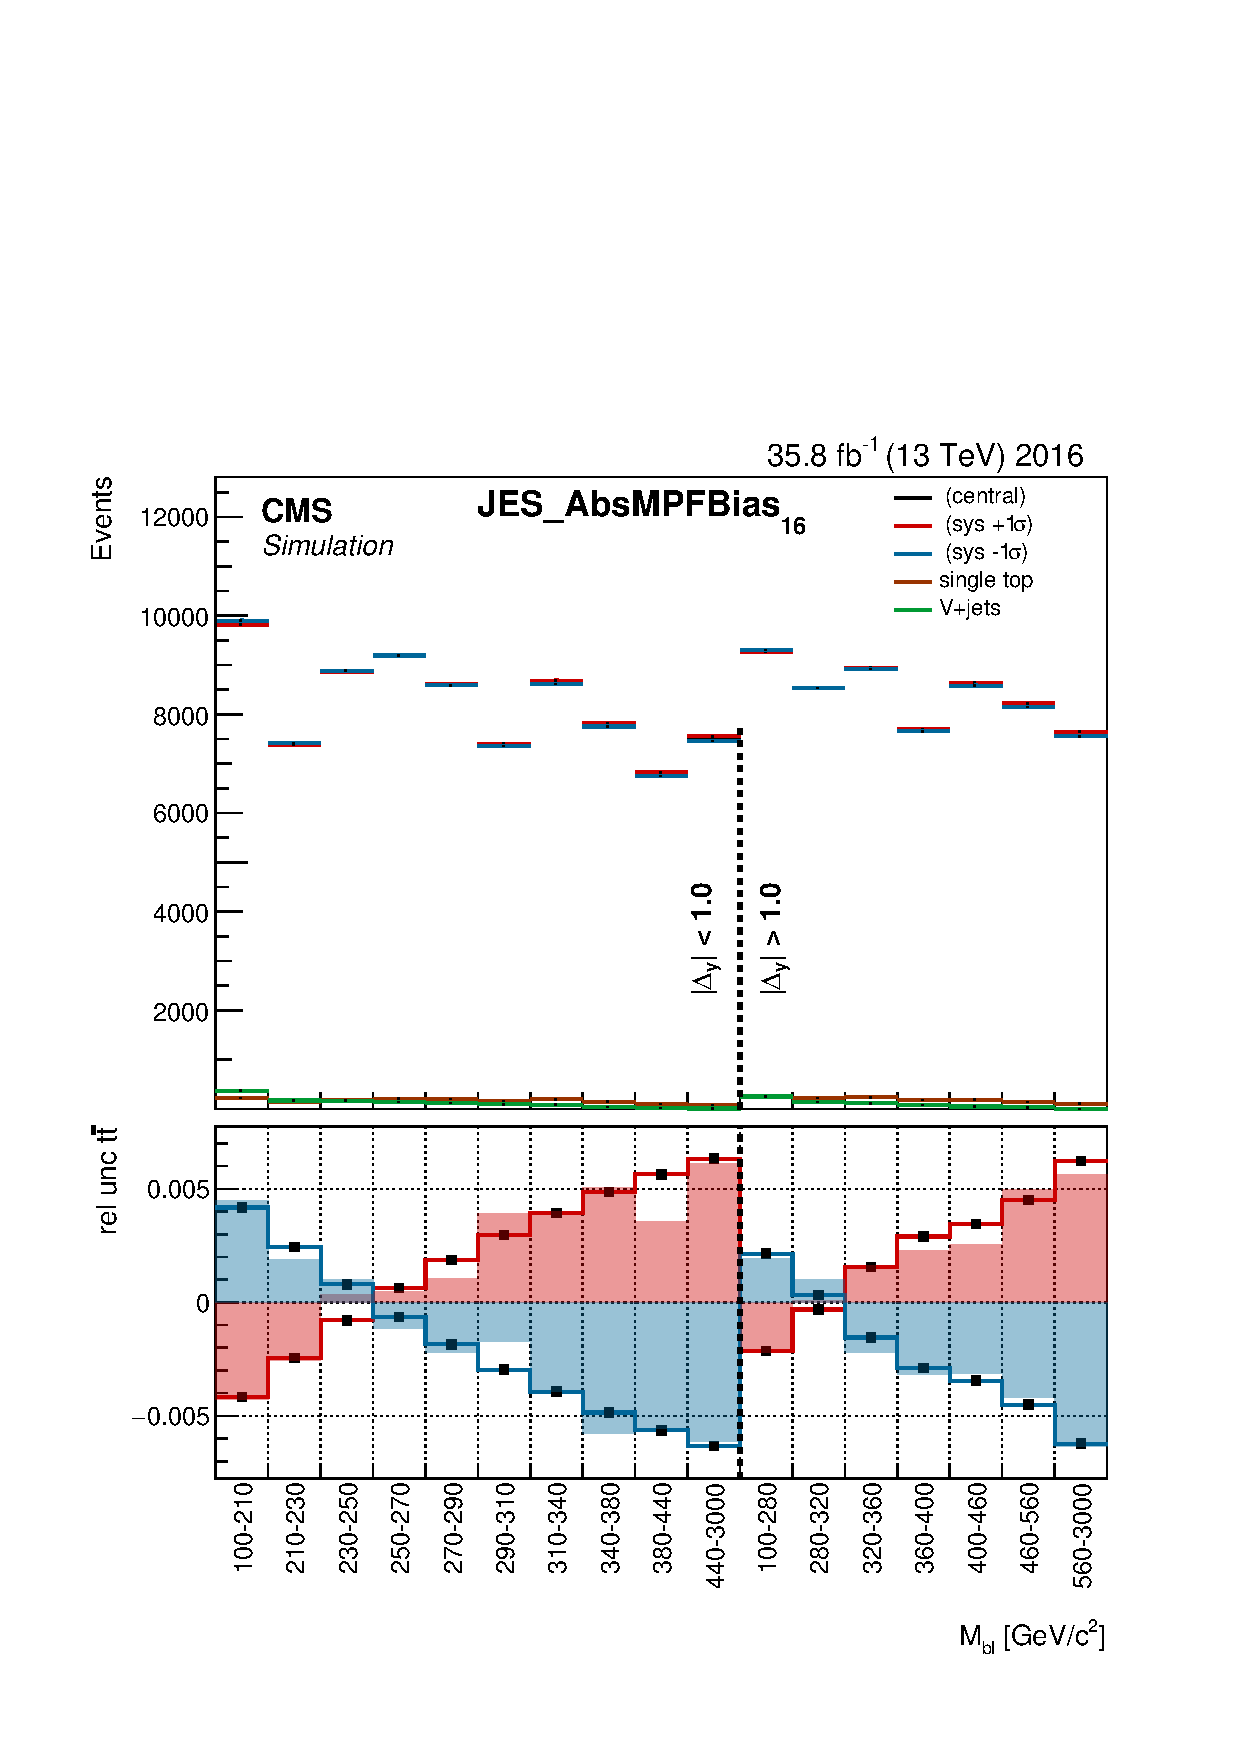
\includegraphics[width=.35\linewidth]{templates/JES_AbsoluteMPFBias_16}\hskip-.5cm
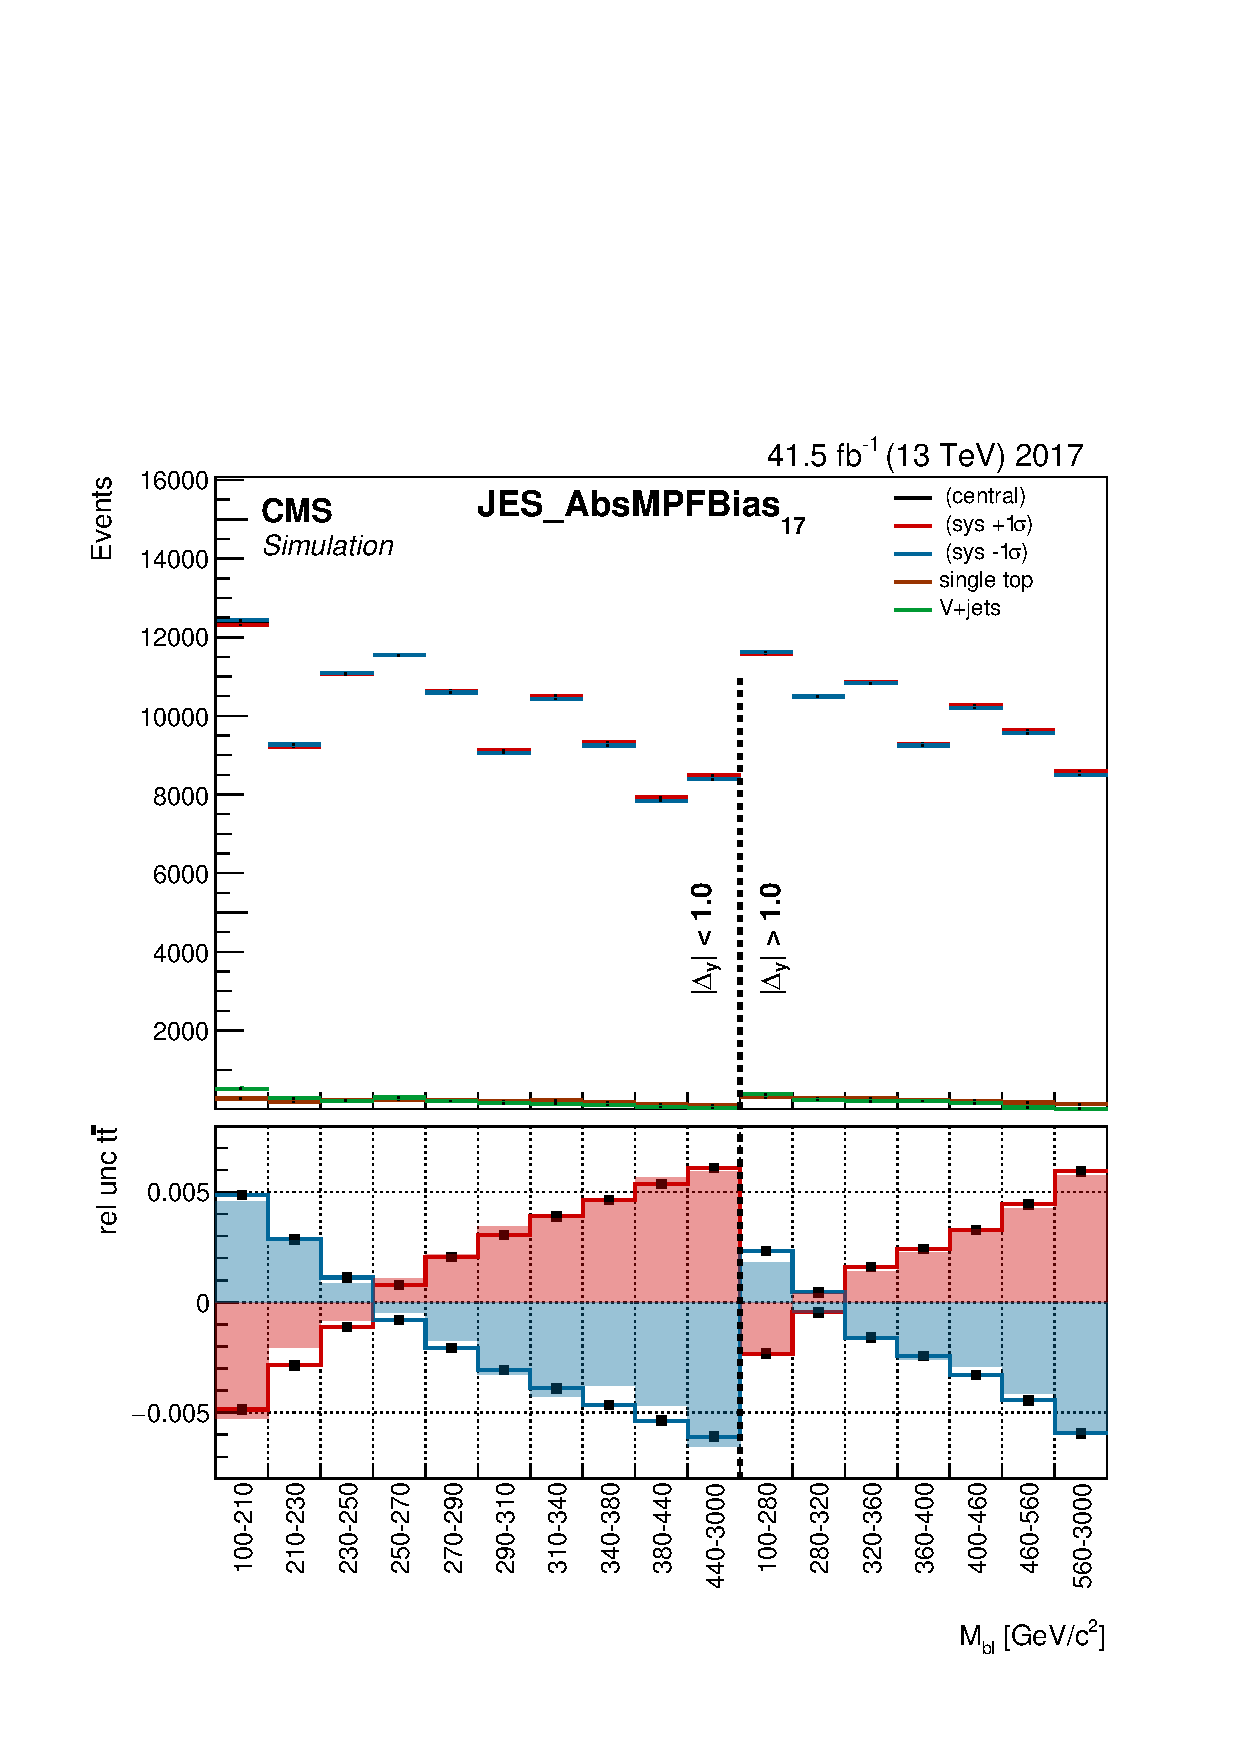
\includegraphics[width=.35\linewidth]{templates/JES_AbsoluteMPFBias_17}\hskip-.5cm
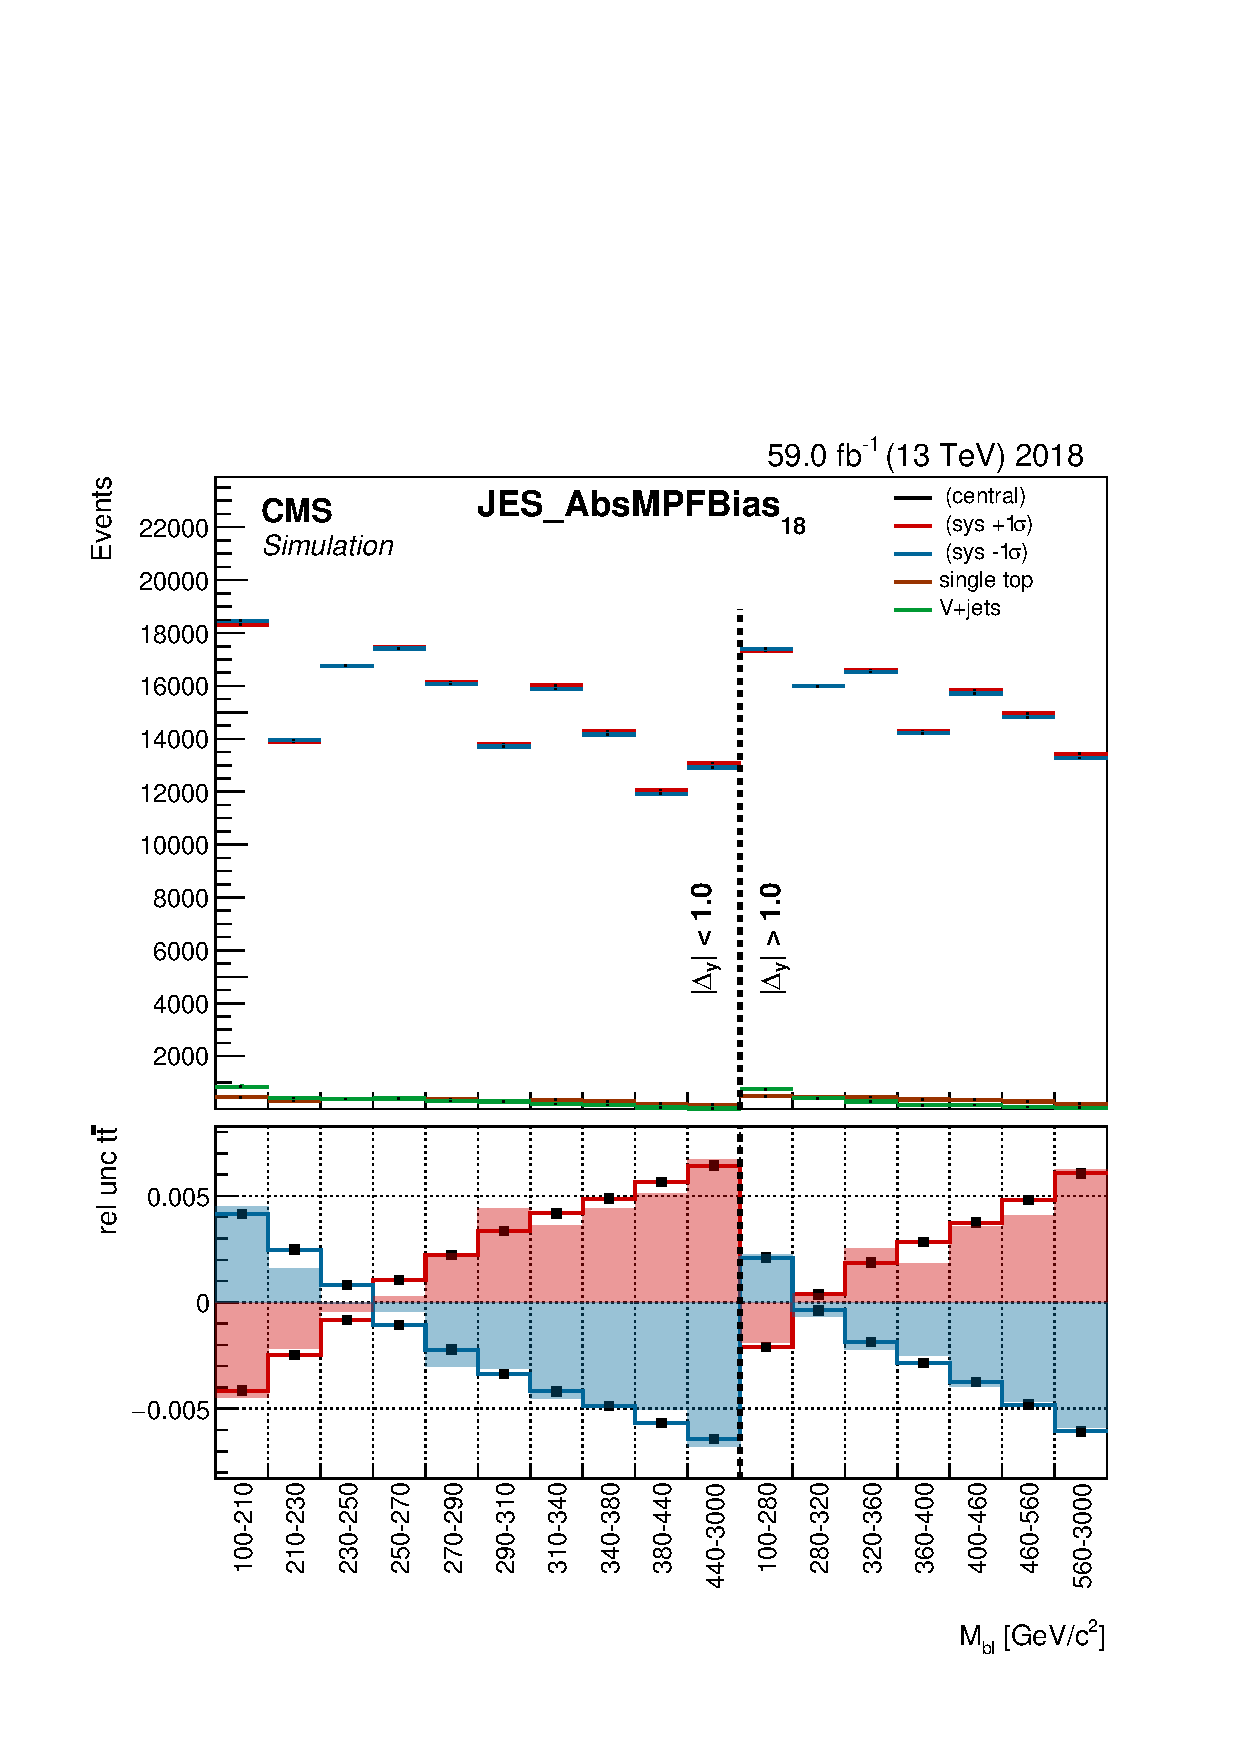
\includegraphics[width=.35\linewidth]{templates/JES_AbsoluteMPFBias_18}
\caption{JES\_AbsoluteMPFBias templates}
\label{fig:JES-AbsoluteMPFBias_template}
\end{figure}

\begin{figure} \centering
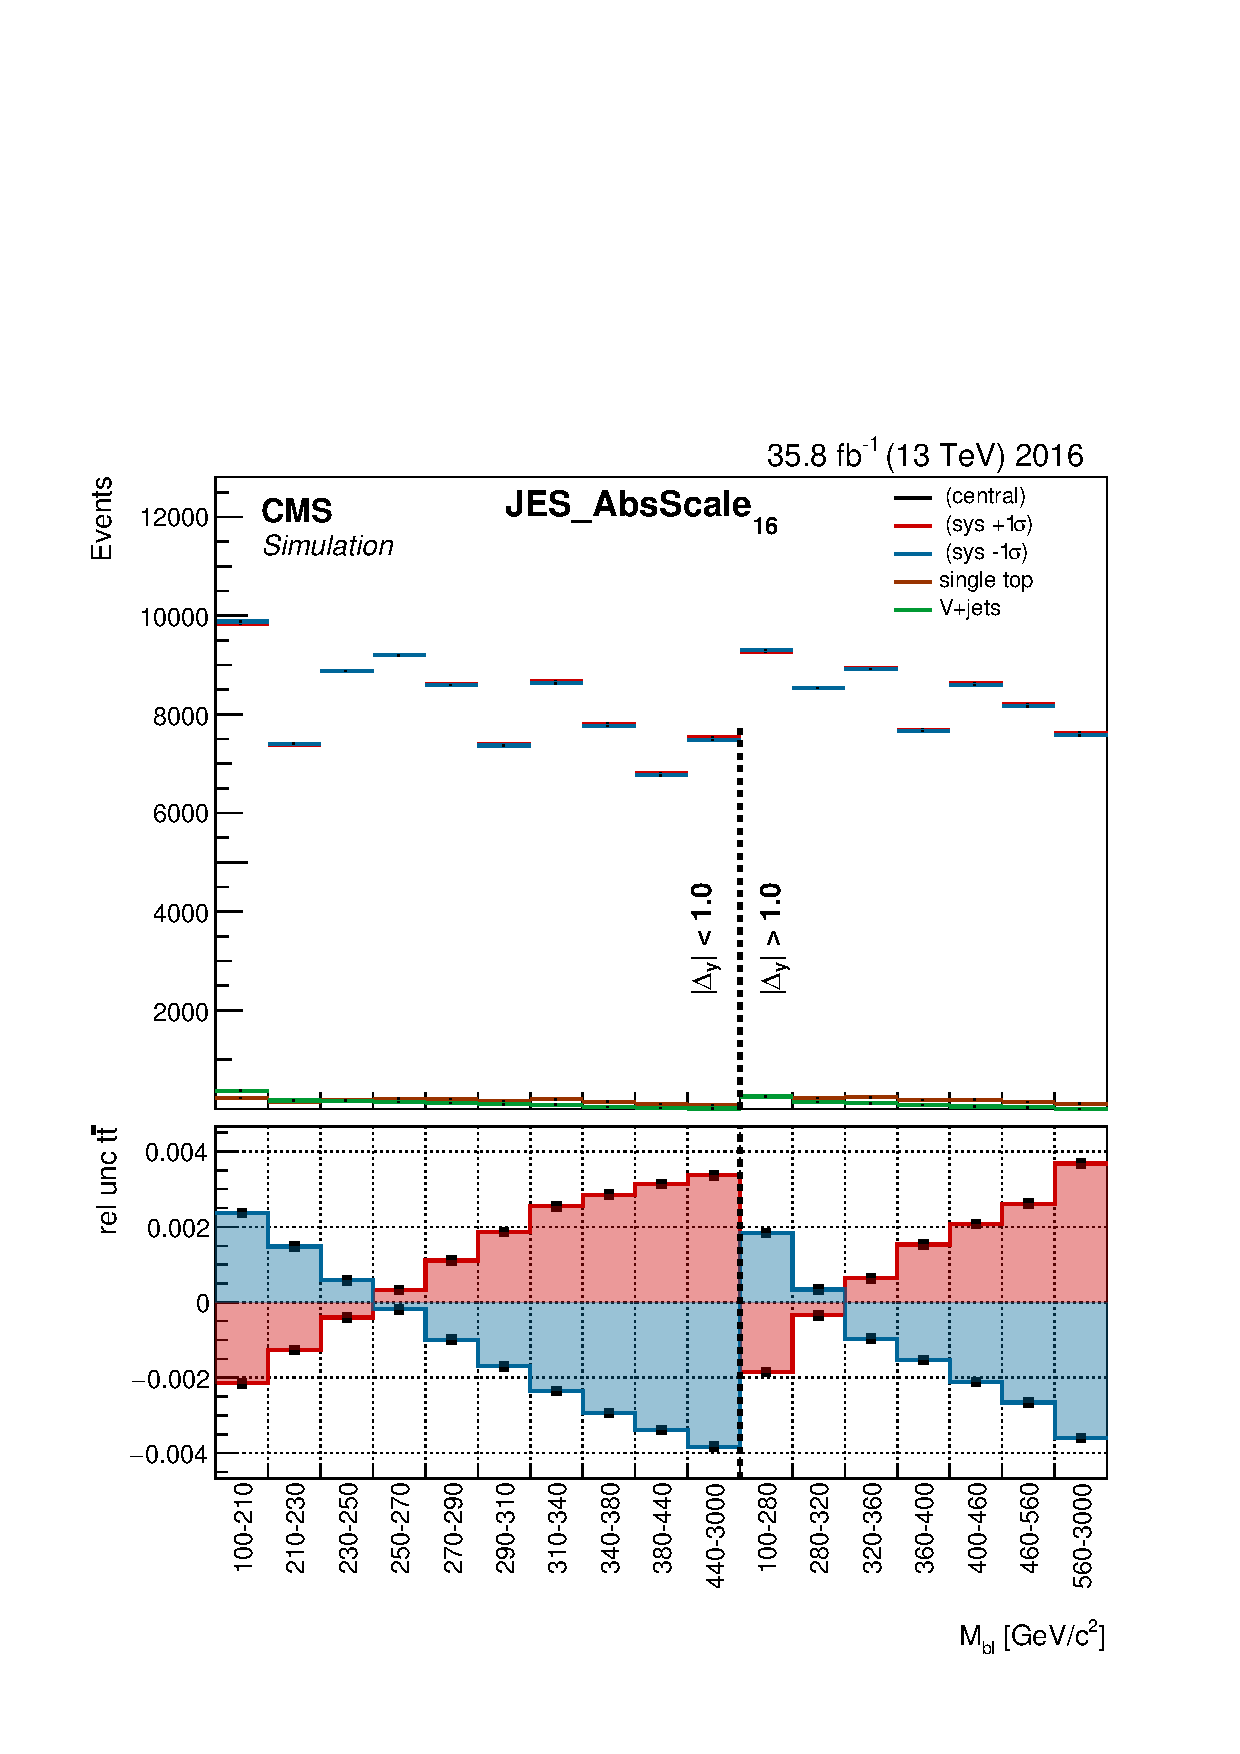
\includegraphics[width=.35\linewidth]{templates/JES_AbsoluteScale_16}\hskip-.5cm
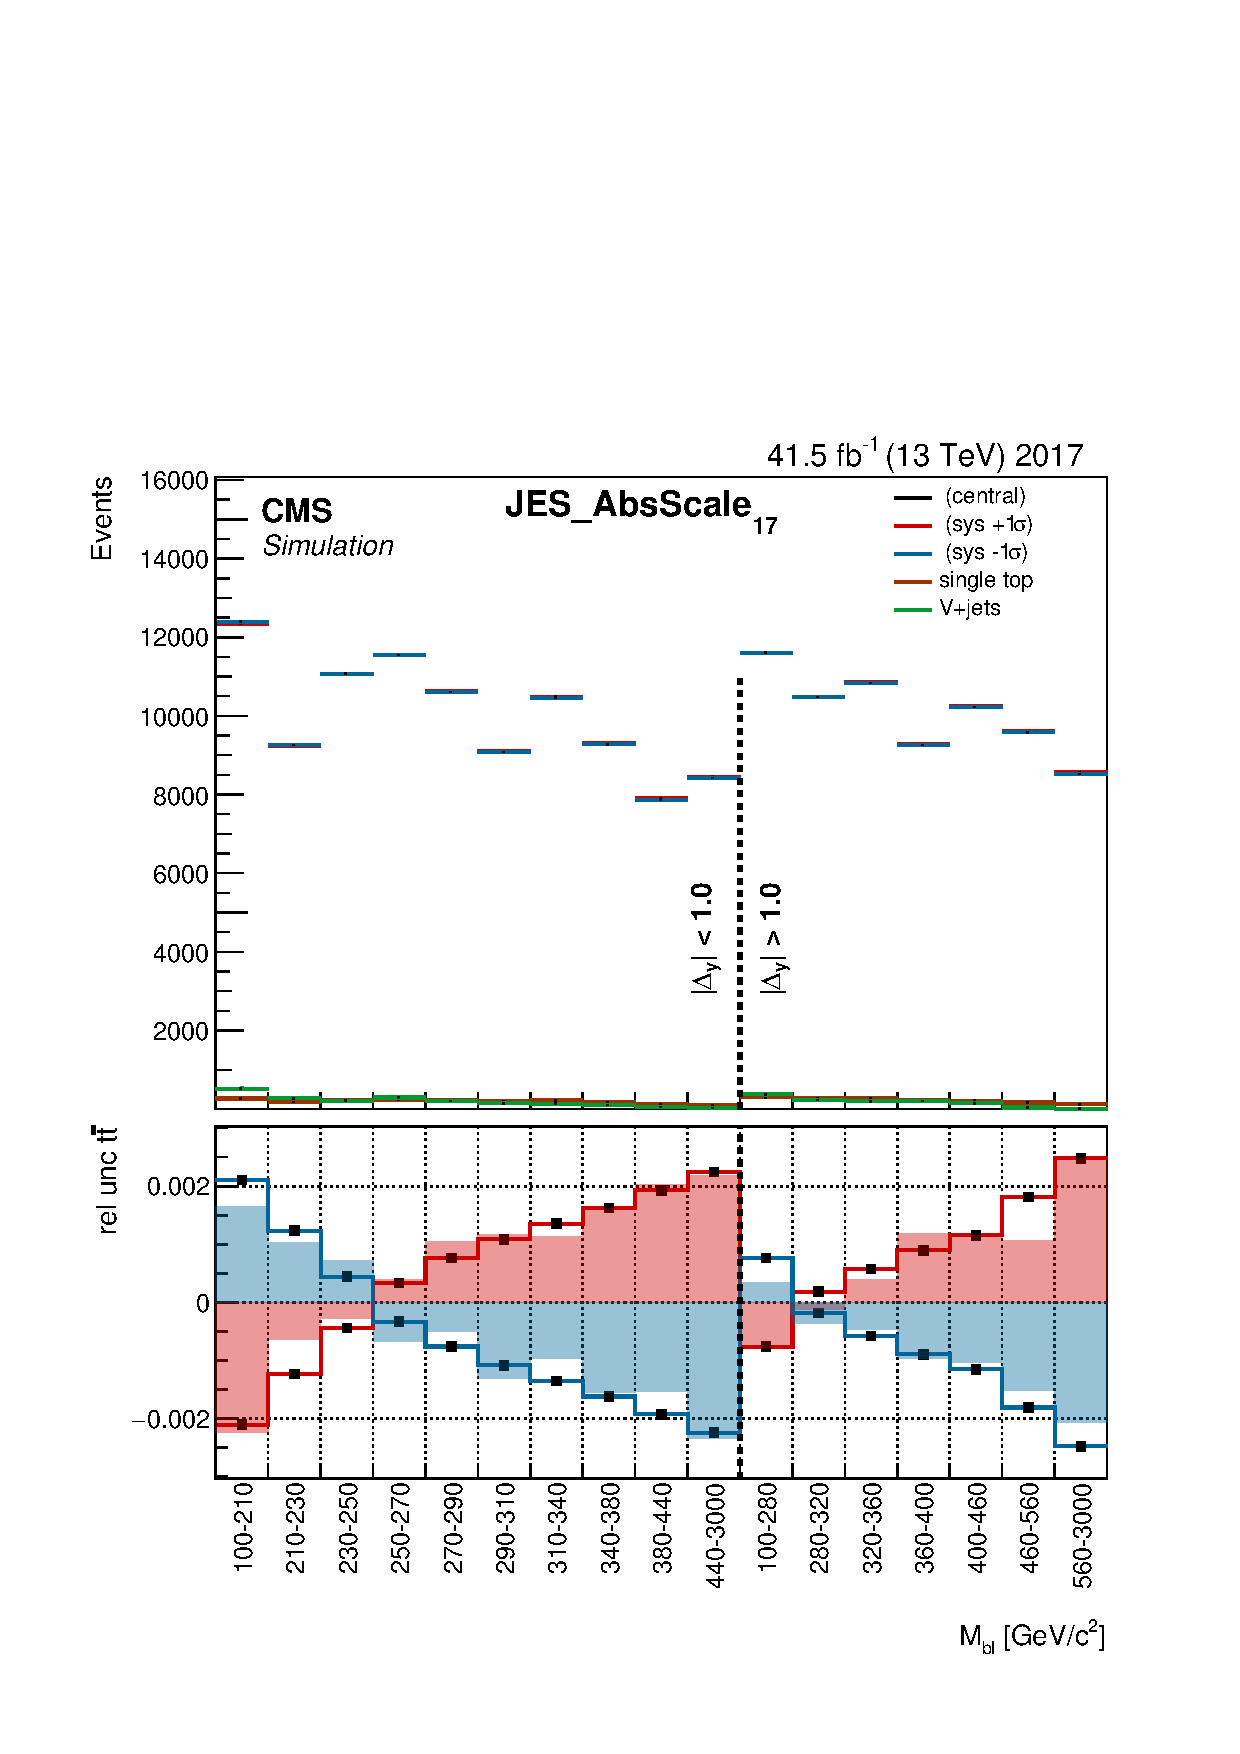
\includegraphics[width=.35\linewidth]{templates/JES_AbsoluteScale_17}\hskip-.5cm
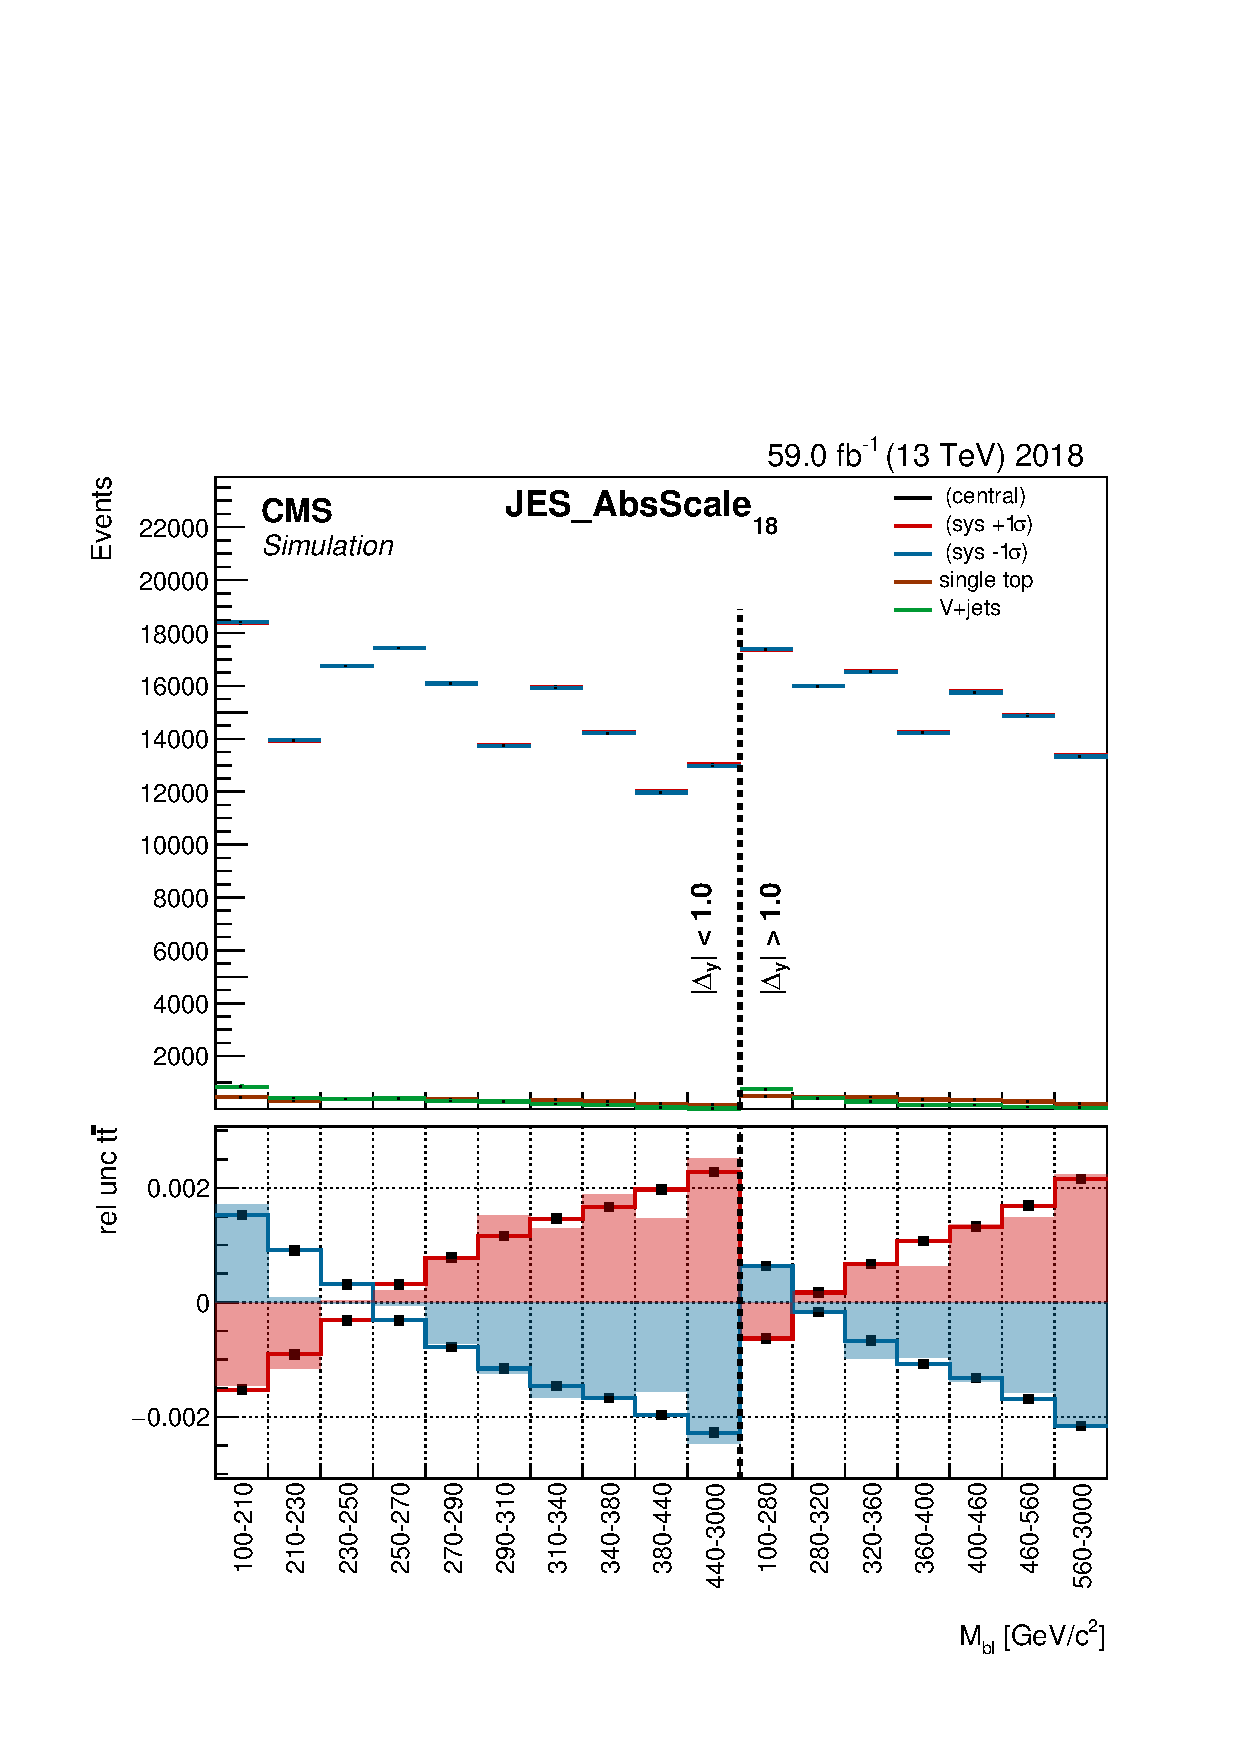
\includegraphics[width=.35\linewidth]{templates/JES_AbsoluteScale_18}
\caption{JES\_AbsoluteScale templates}
\label{fig:JES-AbsoluteScale_template}
\end{figure}

\begin{figure} \centering
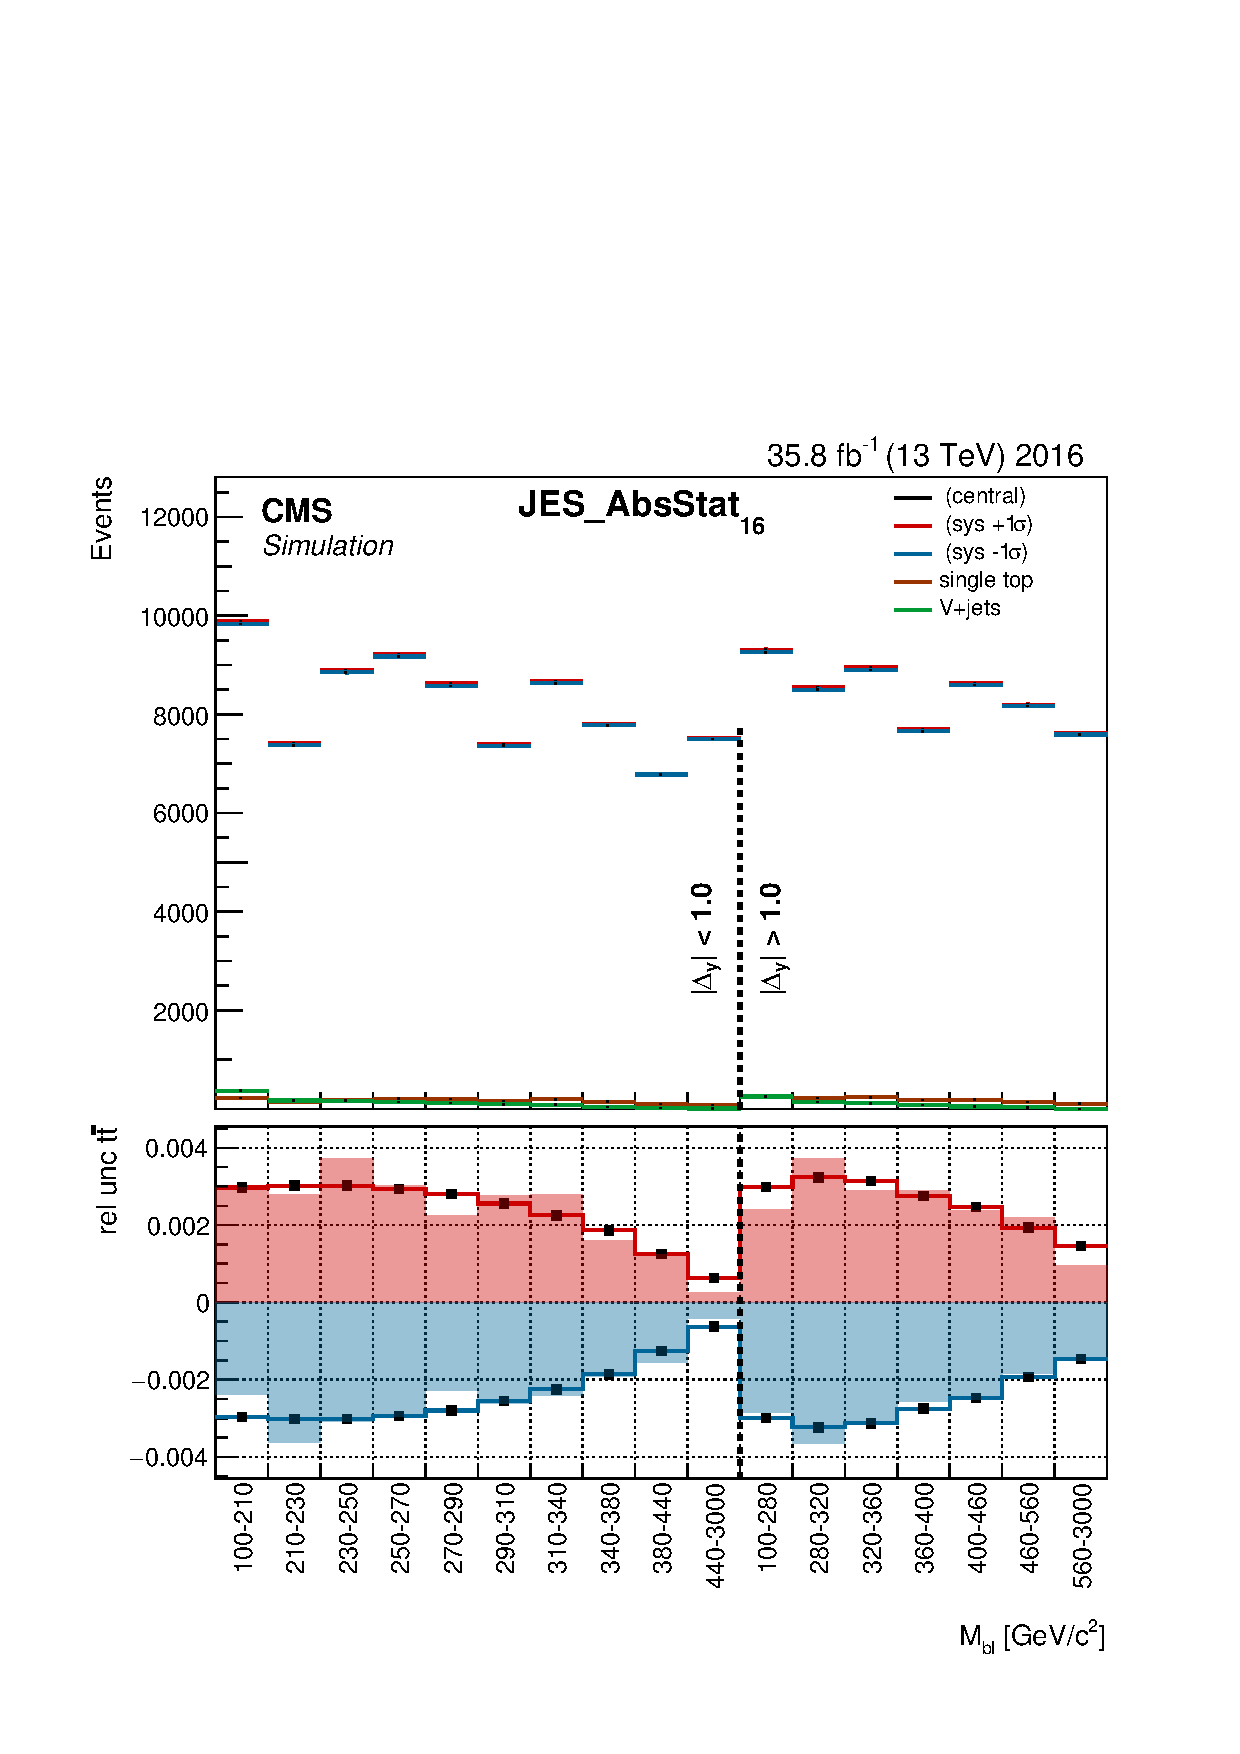
\includegraphics[width=.35\linewidth]{templates/JES_AbsoluteStat_16}\hskip-.5cm
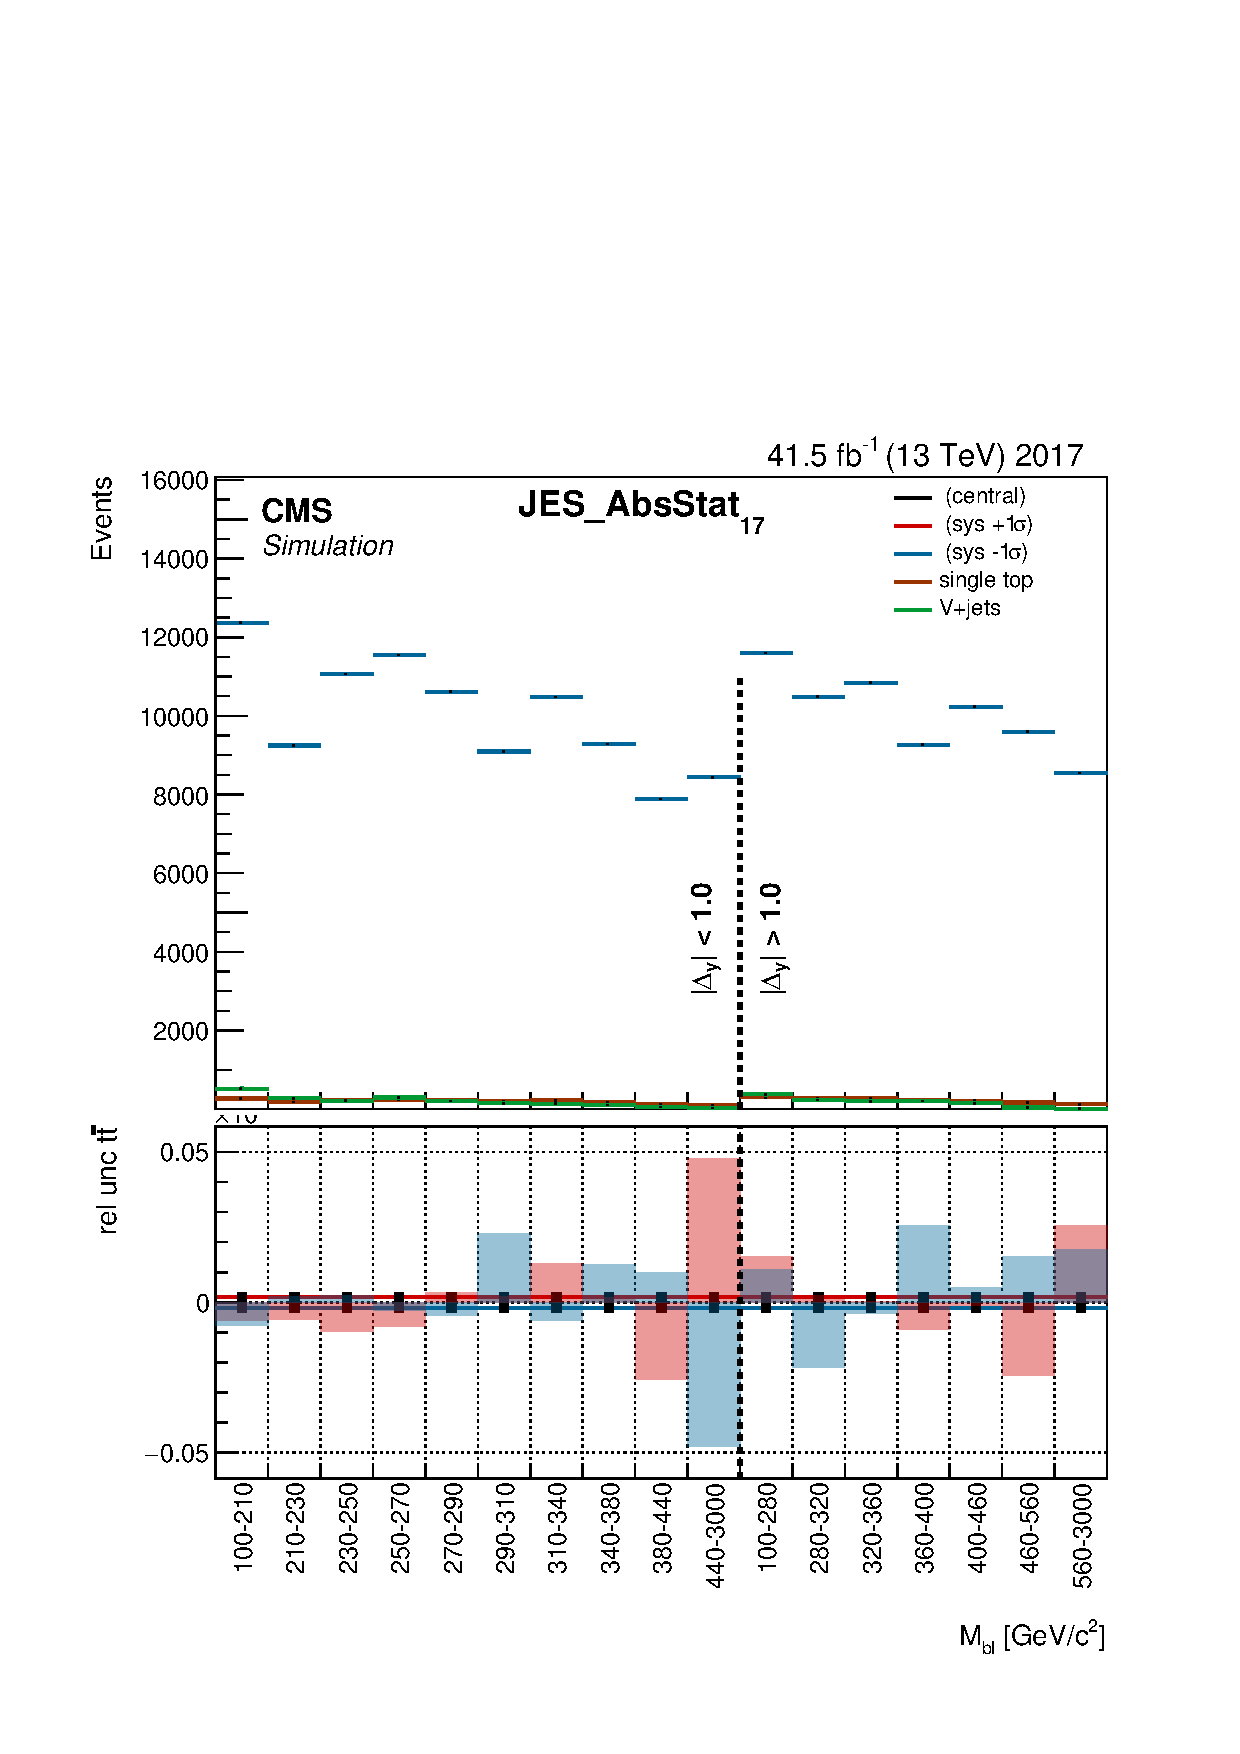
\includegraphics[width=.35\linewidth]{templates/JES_AbsoluteStat_17}\hskip-.5cm
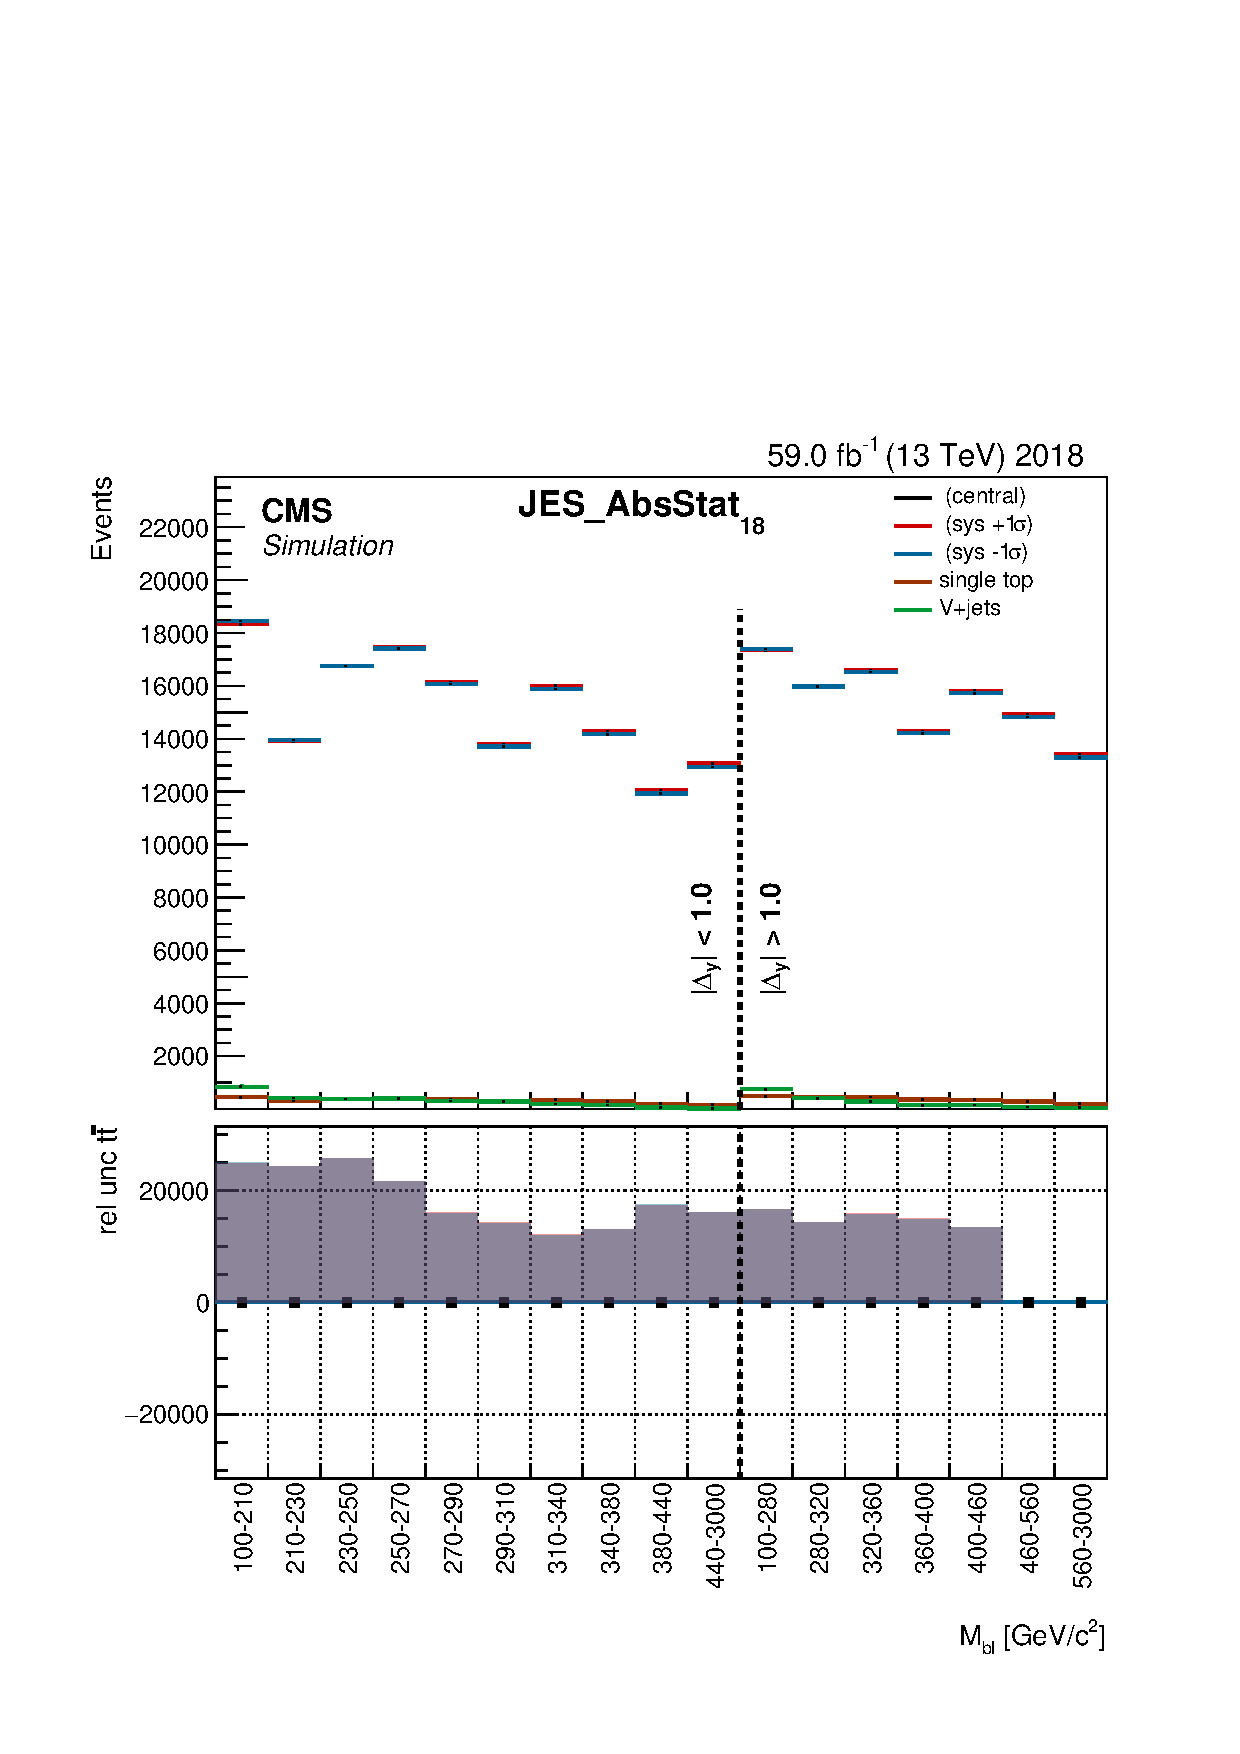
\includegraphics[width=.35\linewidth]{templates/JES_AbsoluteStat_18}
\caption{JES\_AbsoluteStat templates}
\label{fig:JES-AbsoluteStat_template}
\end{figure}

\begin{figure} \centering
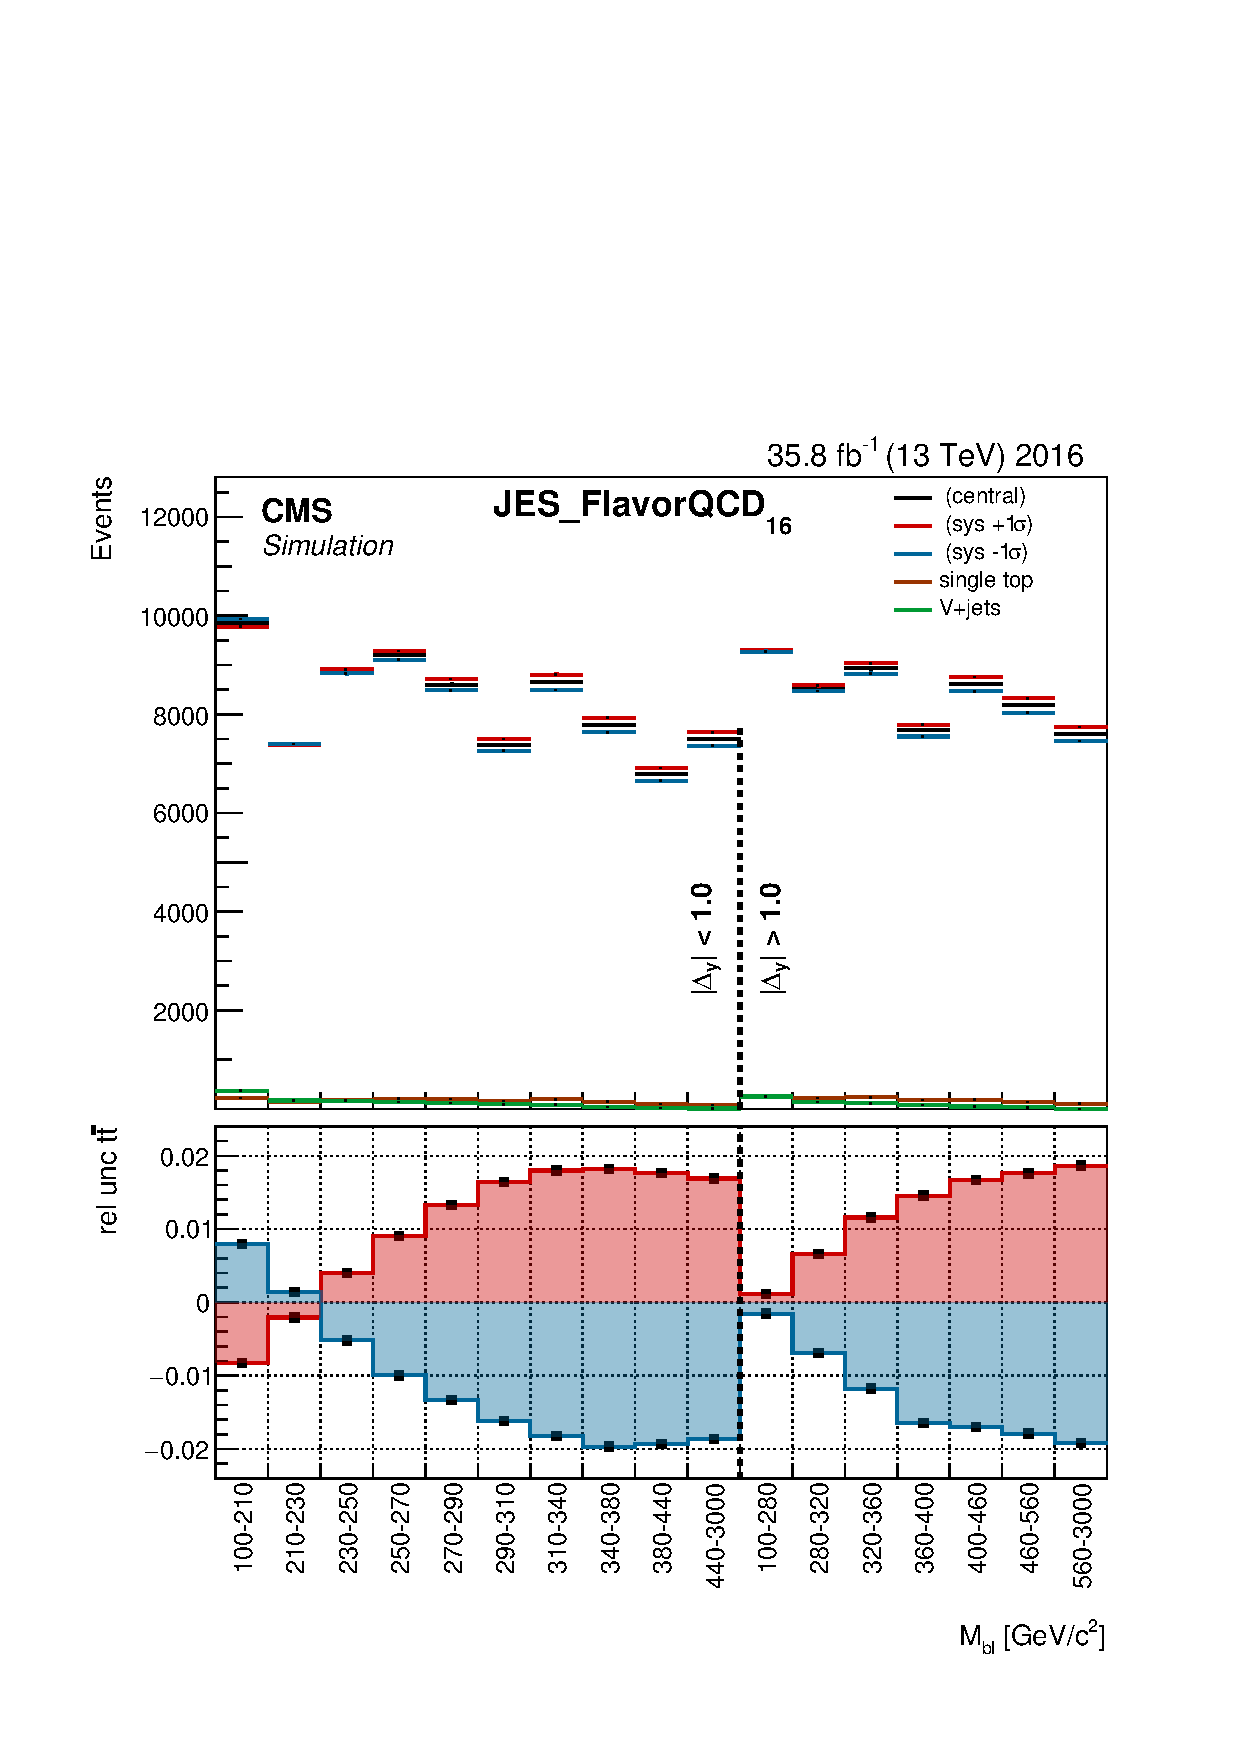
\includegraphics[width=.35\linewidth]{templates/JES_FlavorQCD_16}\hskip-.5cm
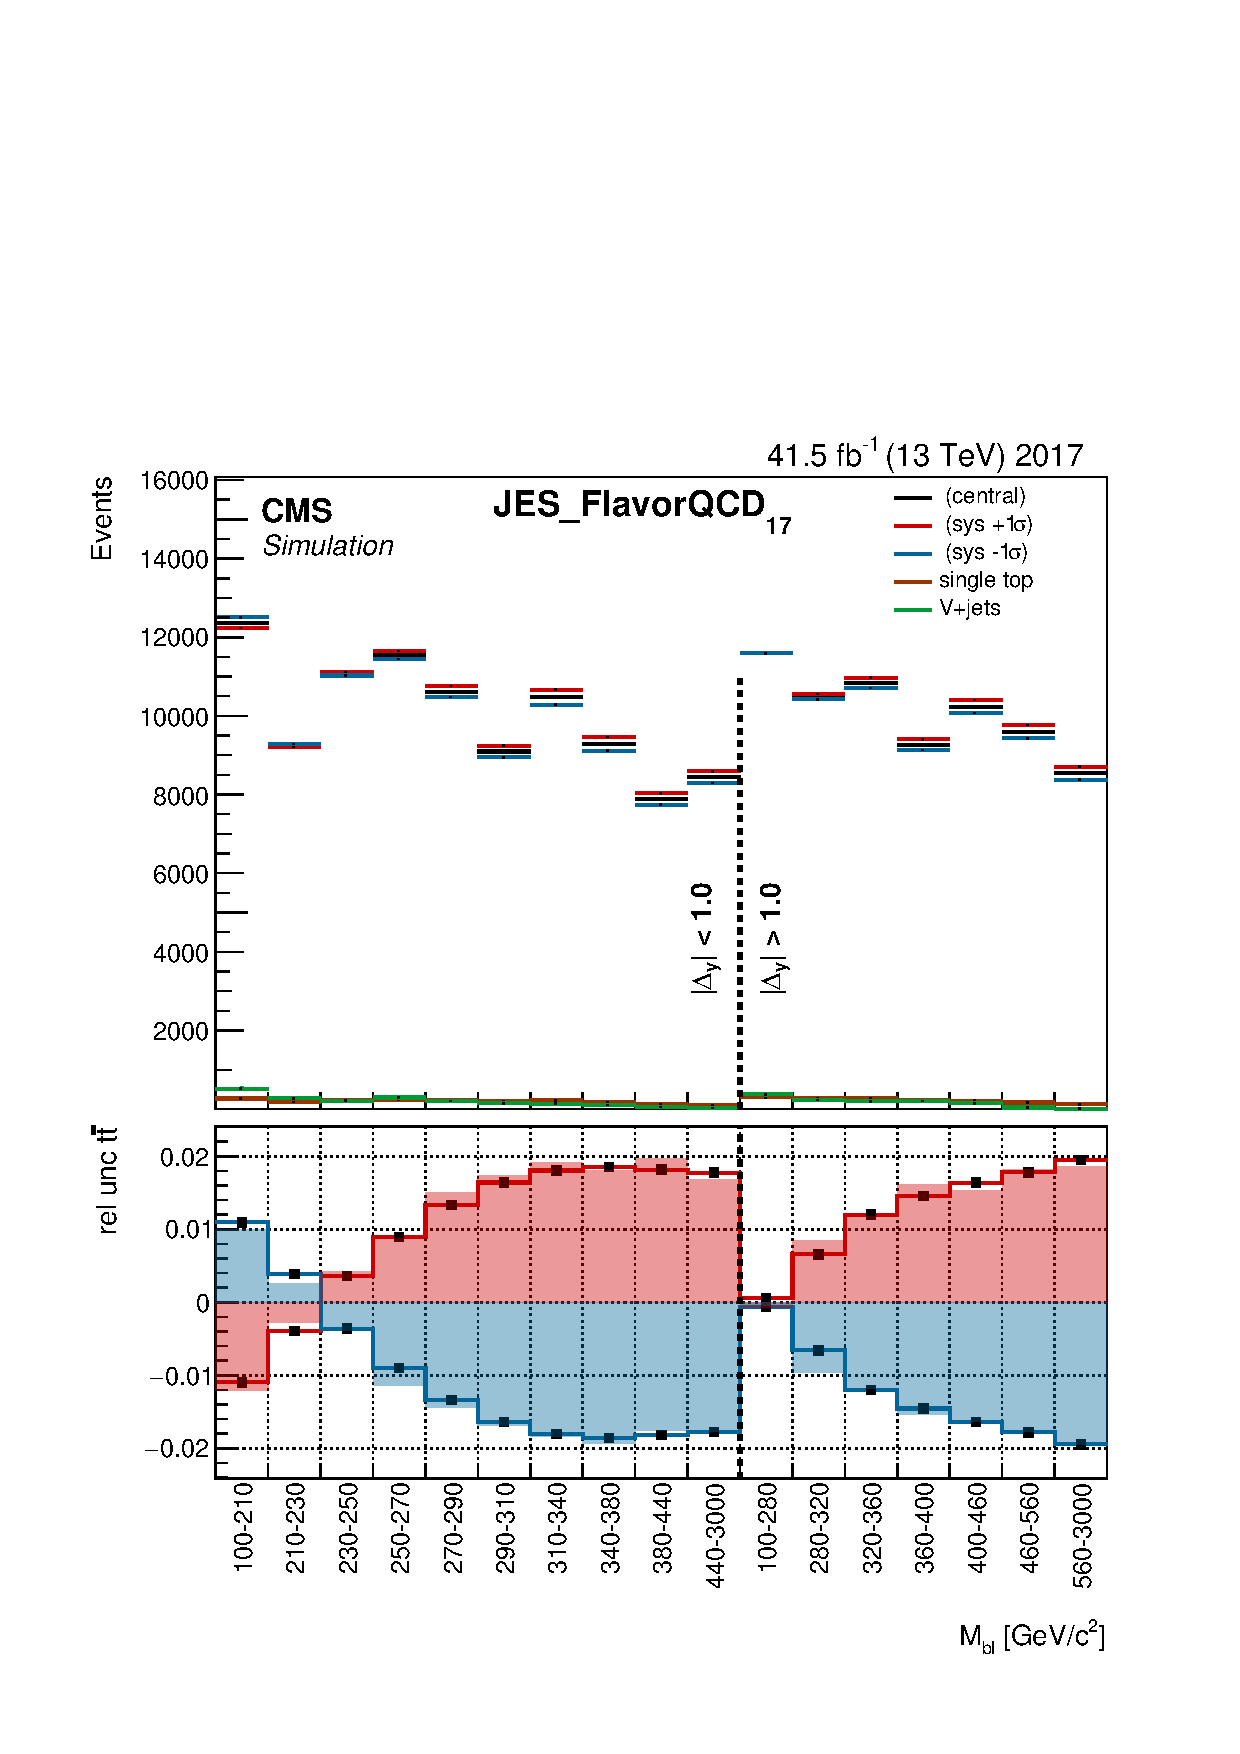
\includegraphics[width=.35\linewidth]{templates/JES_FlavorQCD_17}\hskip-.5cm
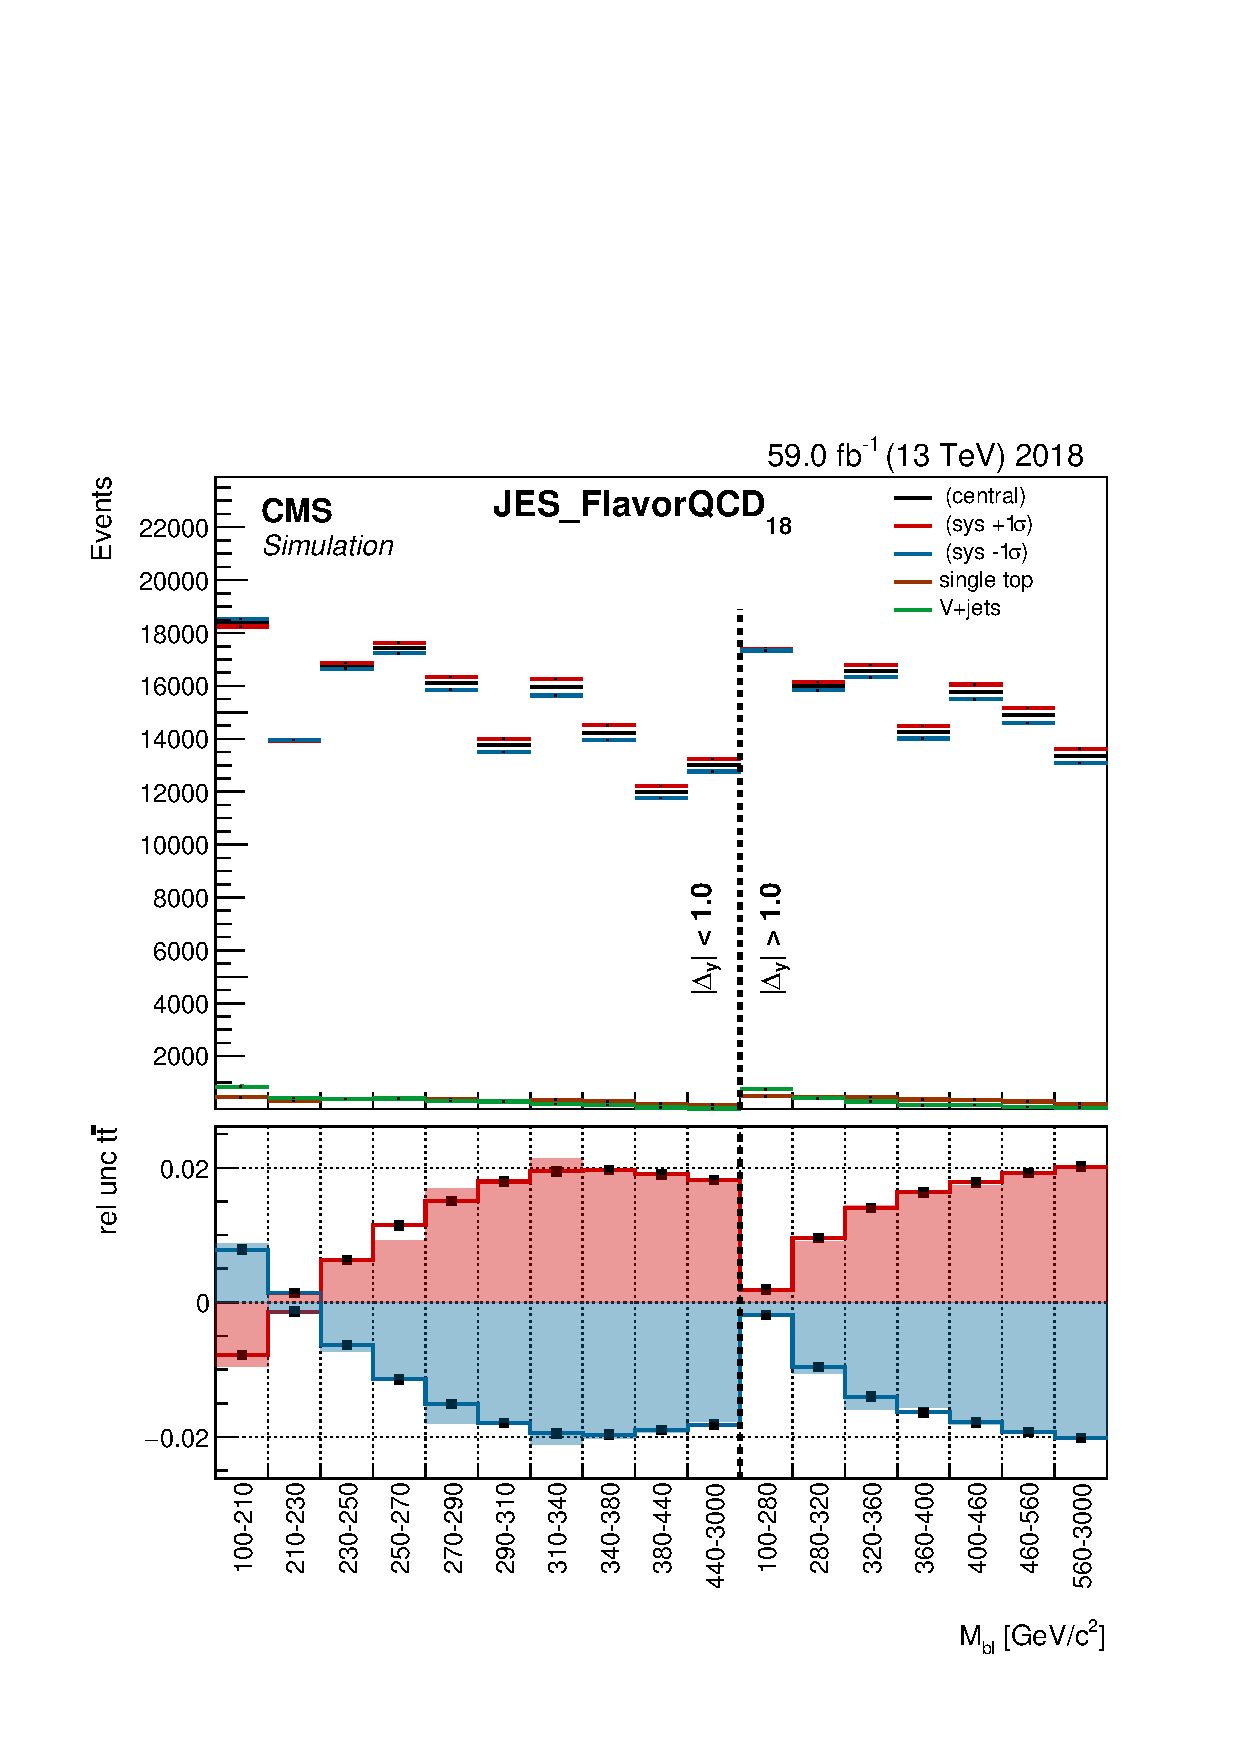
\includegraphics[width=.35\linewidth]{templates/JES_FlavorQCD_18}
\caption{JES\_FlavorQCD templates}
\label{fig:JES-FlavorQCD_template}
\end{figure}

\begin{figure} \centering
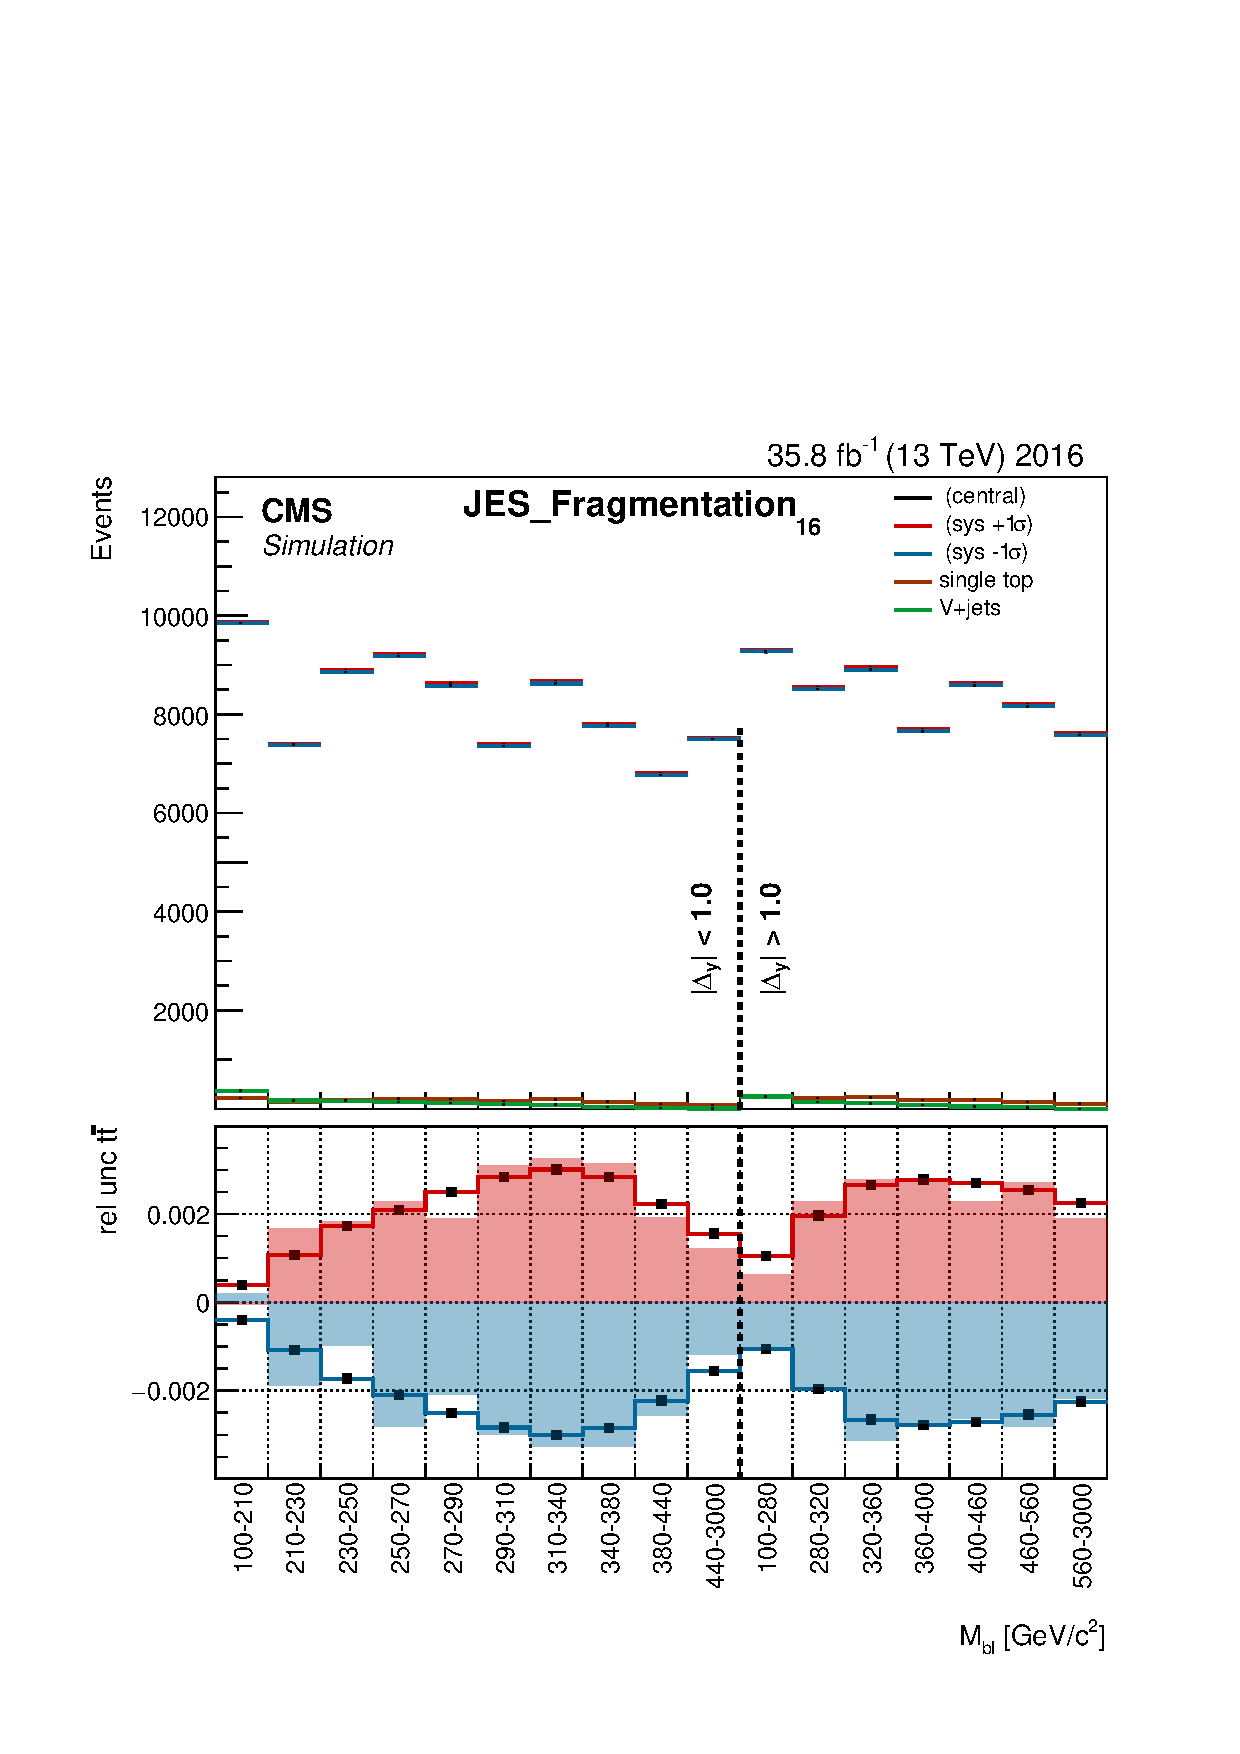
\includegraphics[width=.35\linewidth]{templates/JES_Fragmentation_16}\hskip-.5cm
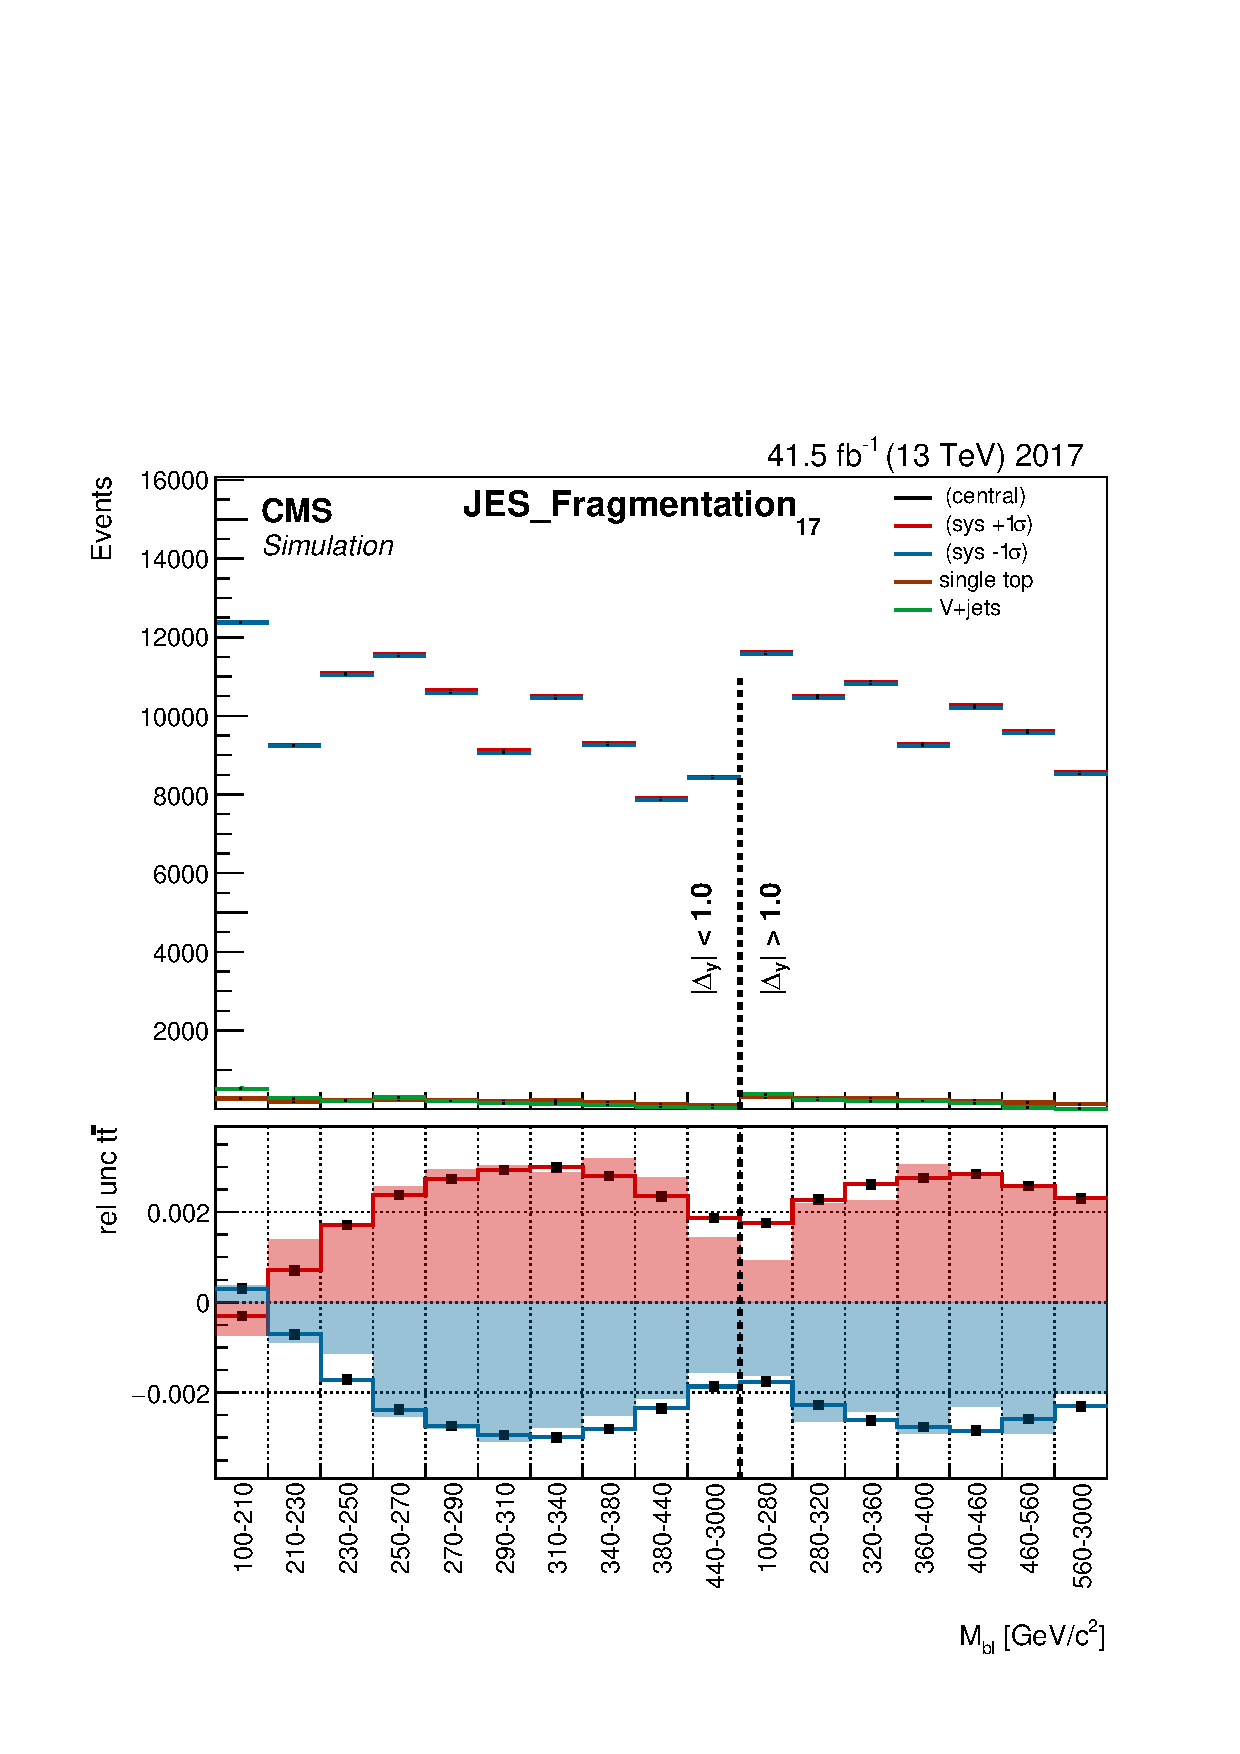
\includegraphics[width=.35\linewidth]{templates/JES_Fragmentation_17}\hskip-.5cm
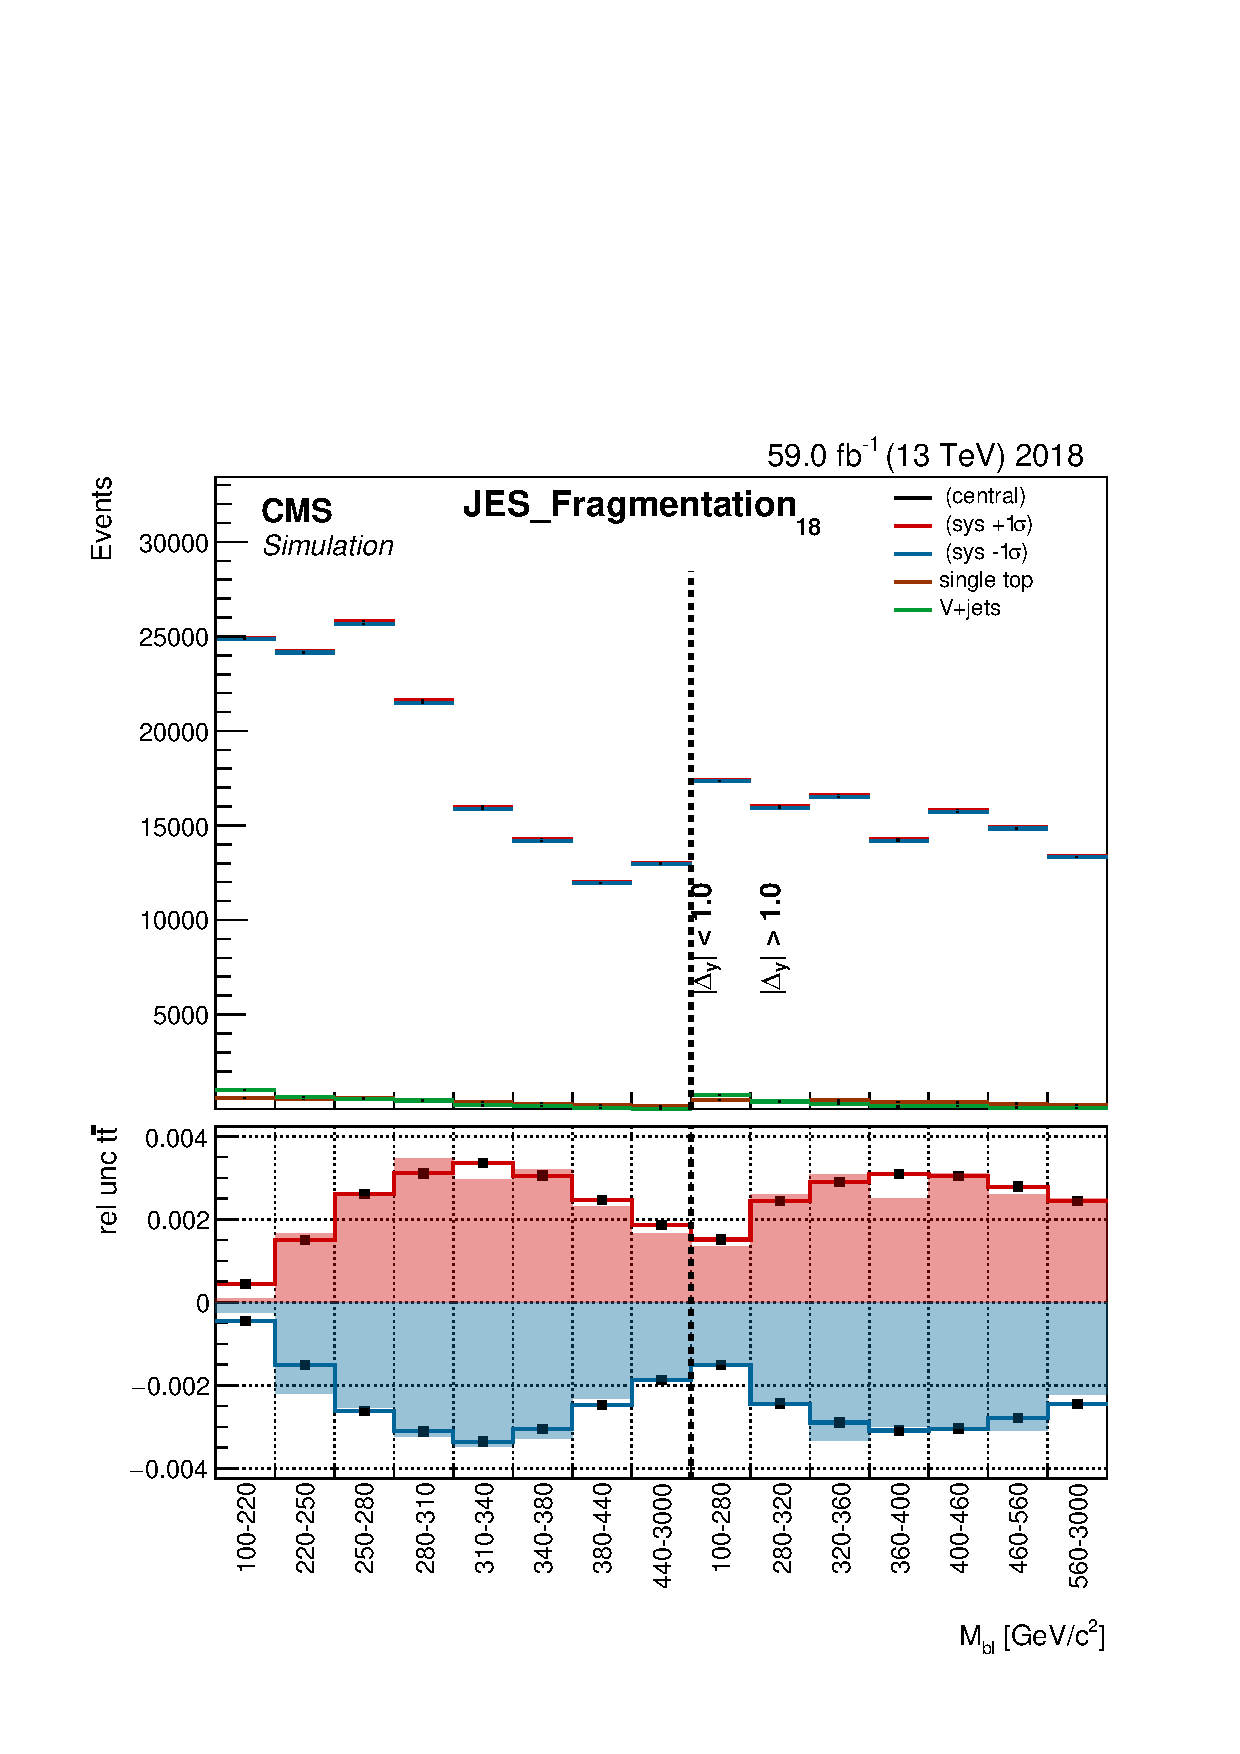
\includegraphics[width=.35\linewidth]{templates/JES_Fragmentation_18}
\caption{JES\_Fragmentation templates}
\label{fig:JES-Fragmentation_template}
\end{figure}

\begin{figure} \centering
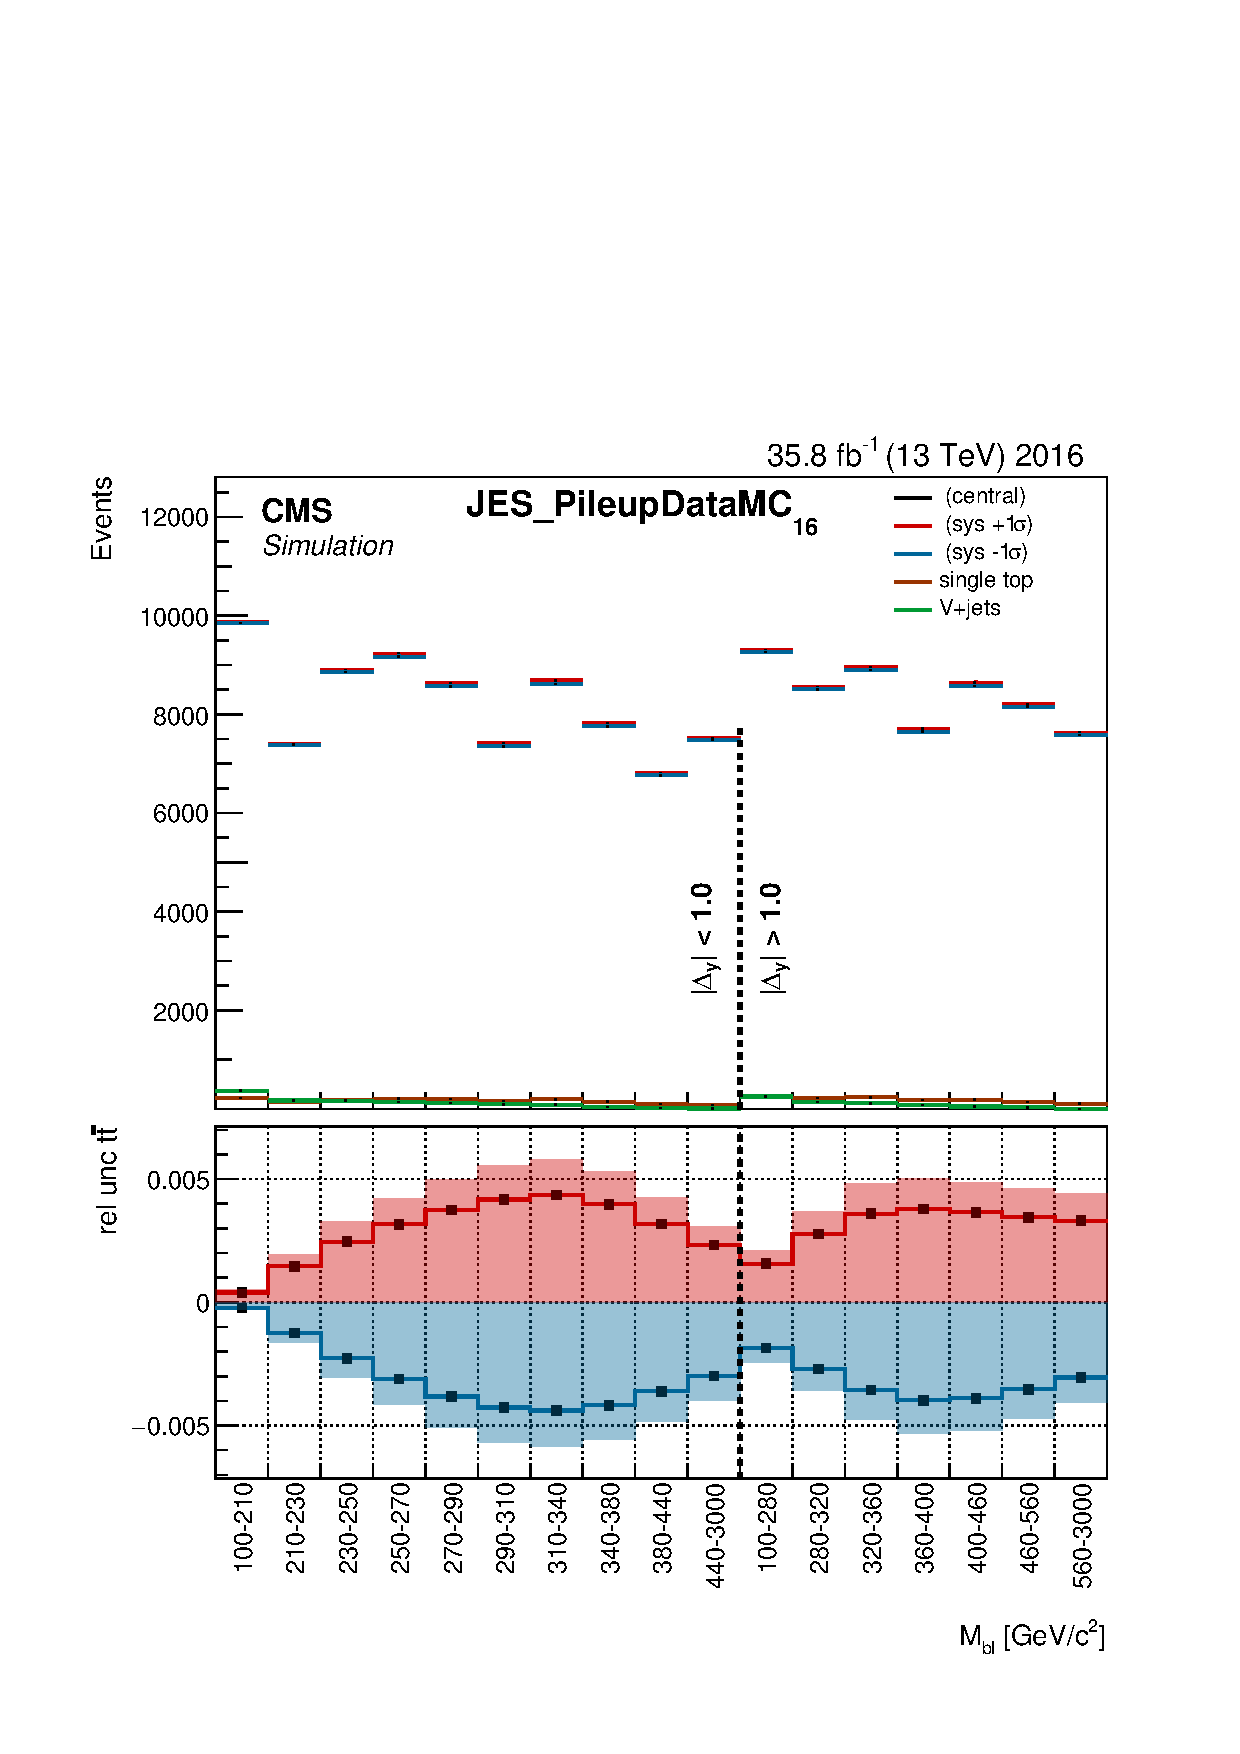
\includegraphics[width=.35\linewidth]{templates/JES_PileupDataMC_16}\hskip-.5cm
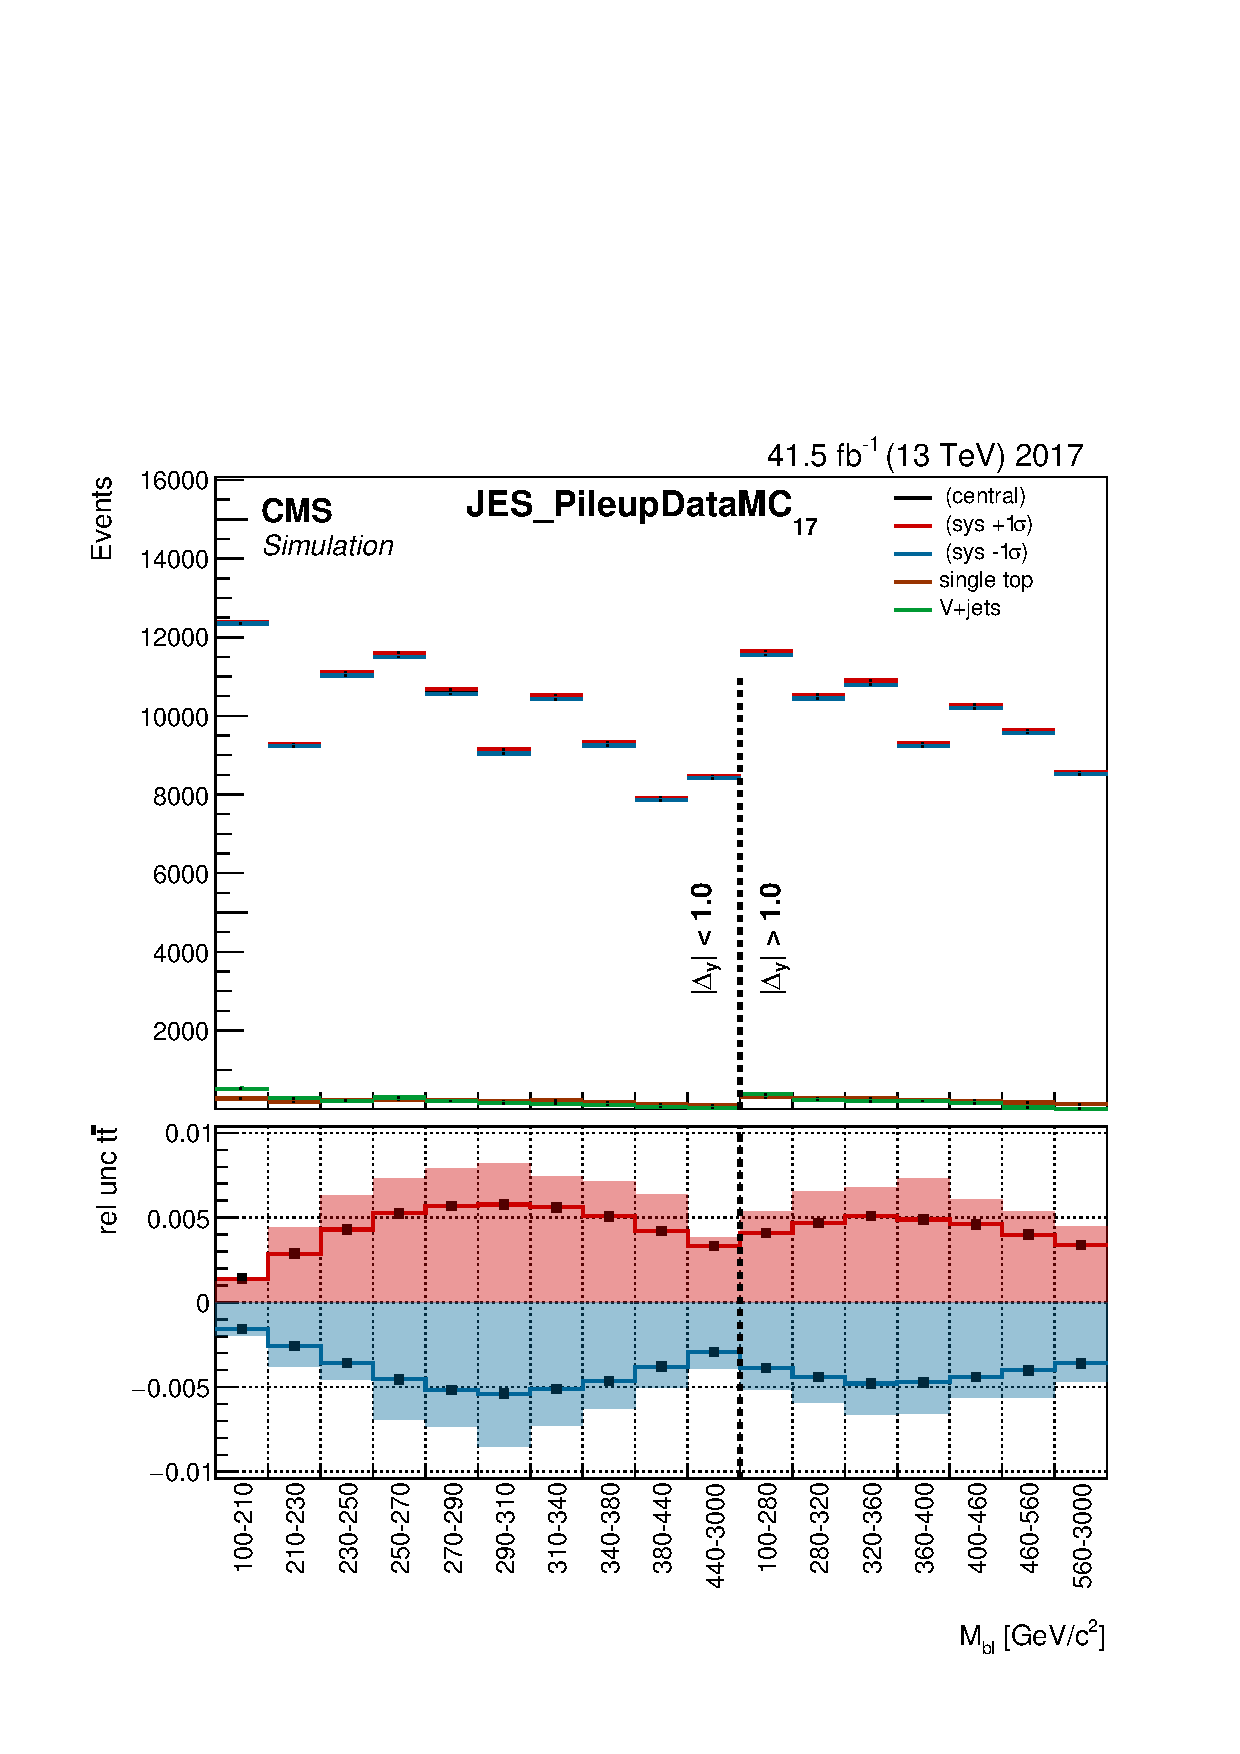
\includegraphics[width=.35\linewidth]{templates/JES_PileupDataMC_17}\hskip-.5cm
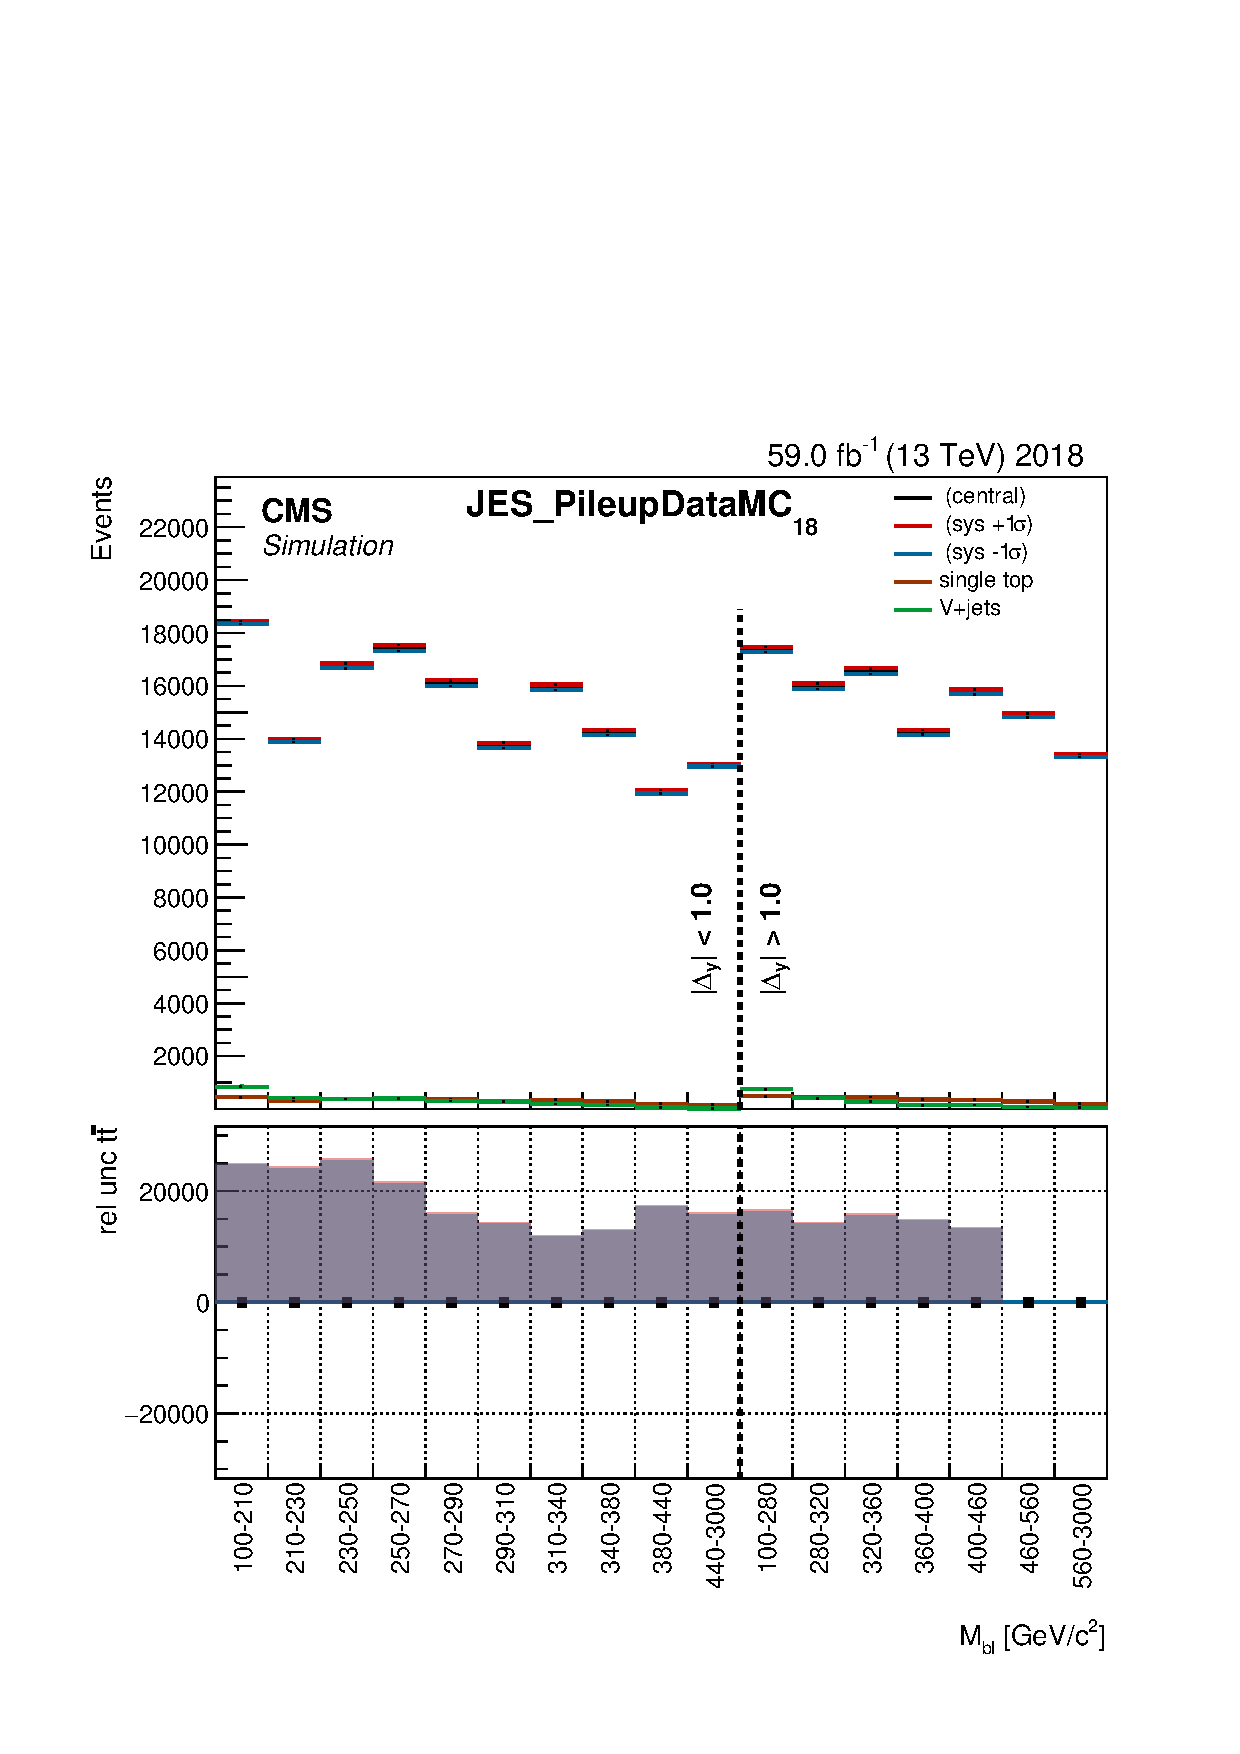
\includegraphics[width=.35\linewidth]{templates/JES_PileupDataMC_18}
\caption{JES\_PileupDataMC templates}
\label{fig:JES-PileupDataMC_template}
\end{figure}

\begin{figure} \centering
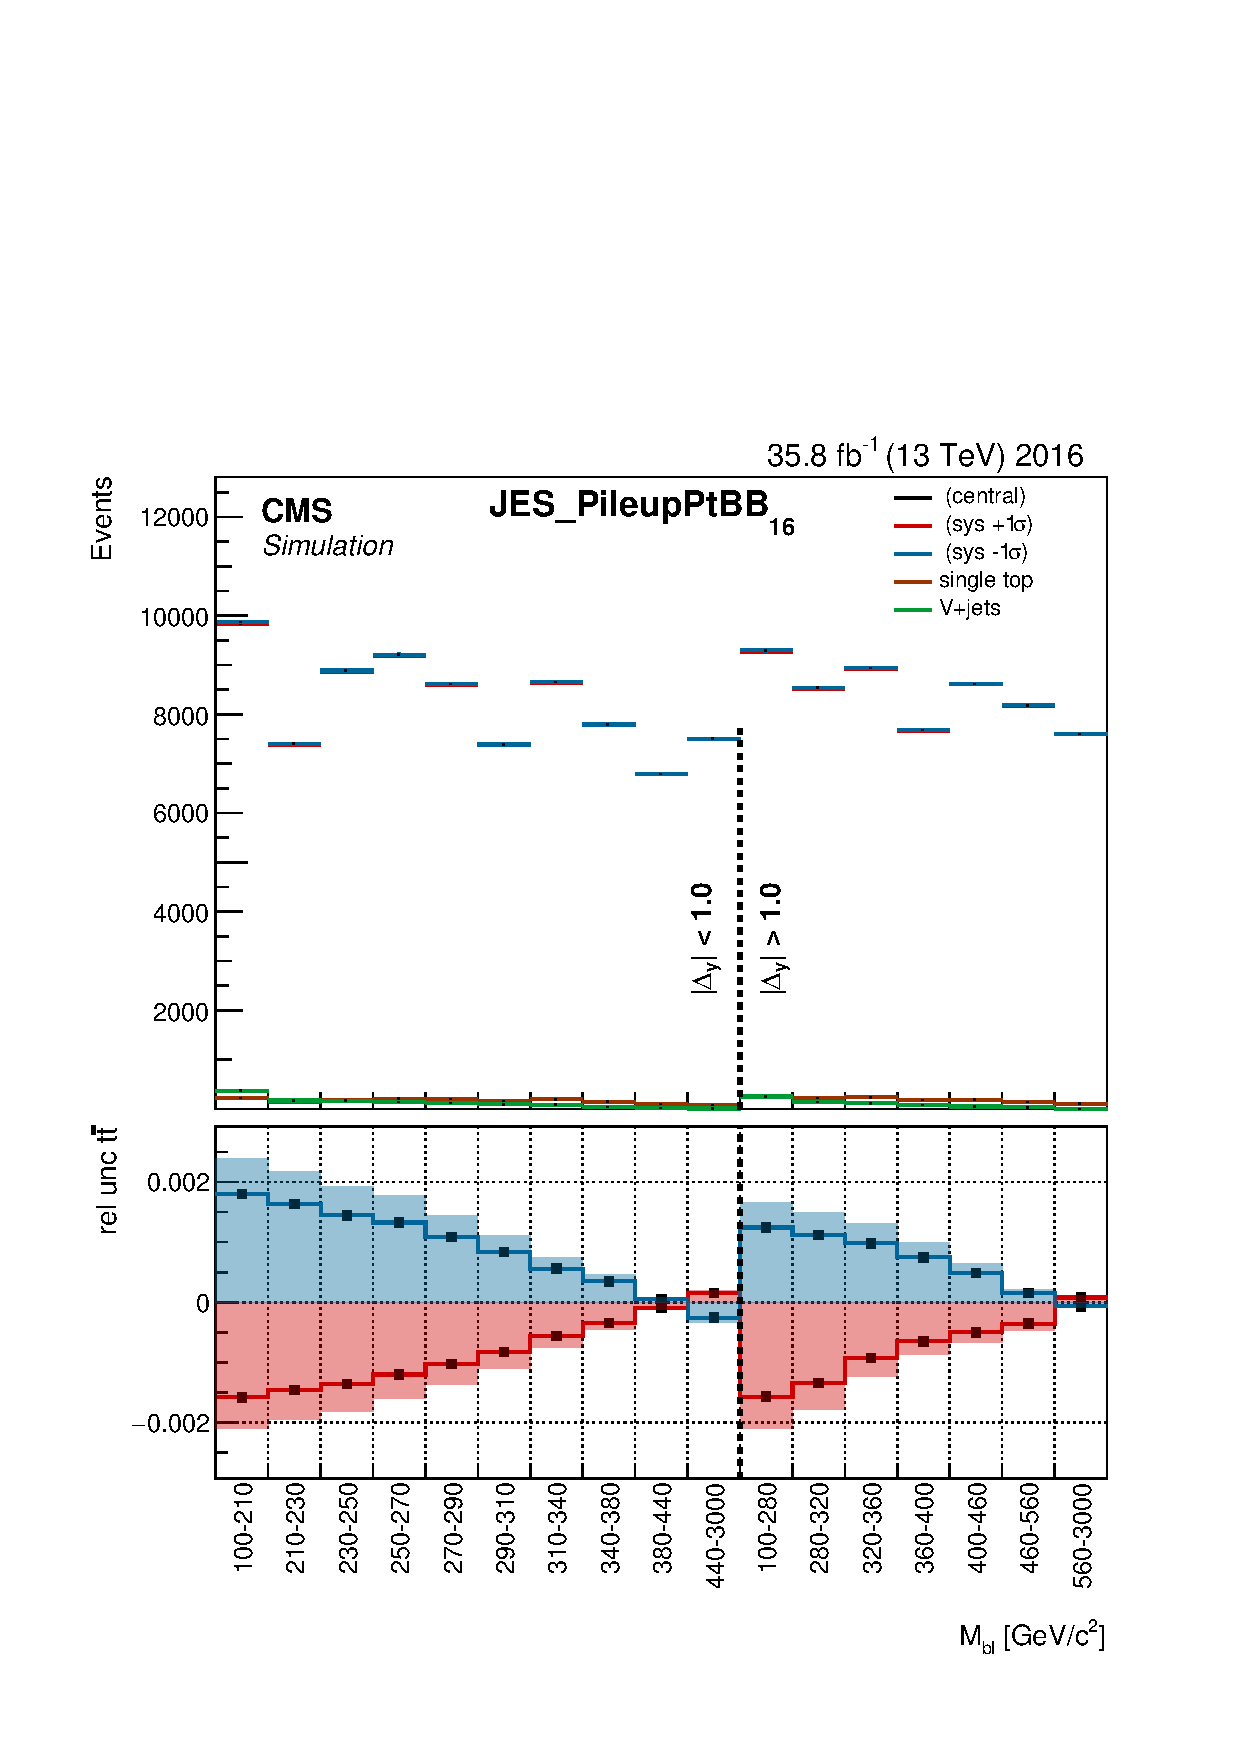
\includegraphics[width=.35\linewidth]{templates/JES_PileupPtBB_16}\hskip-.5cm
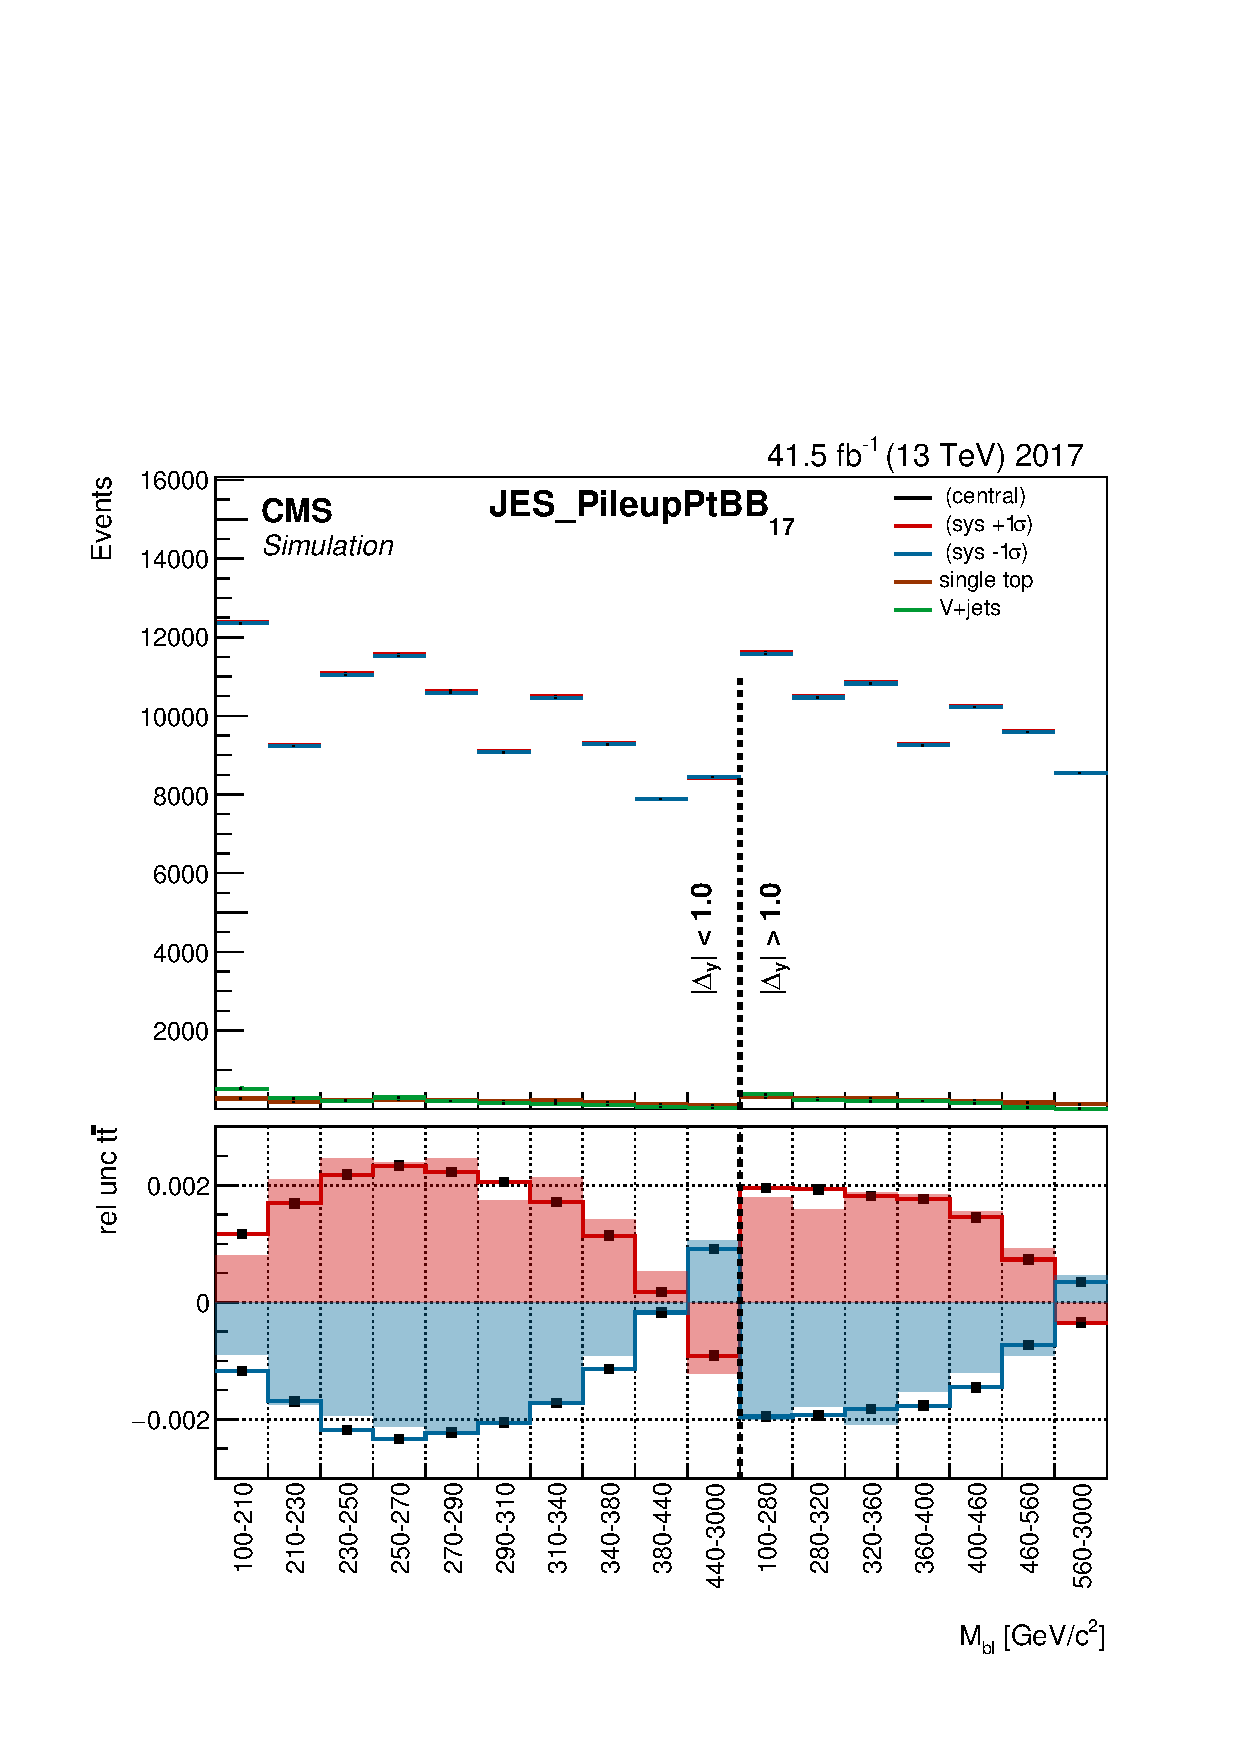
\includegraphics[width=.35\linewidth]{templates/JES_PileupPtBB_17}\hskip-.5cm
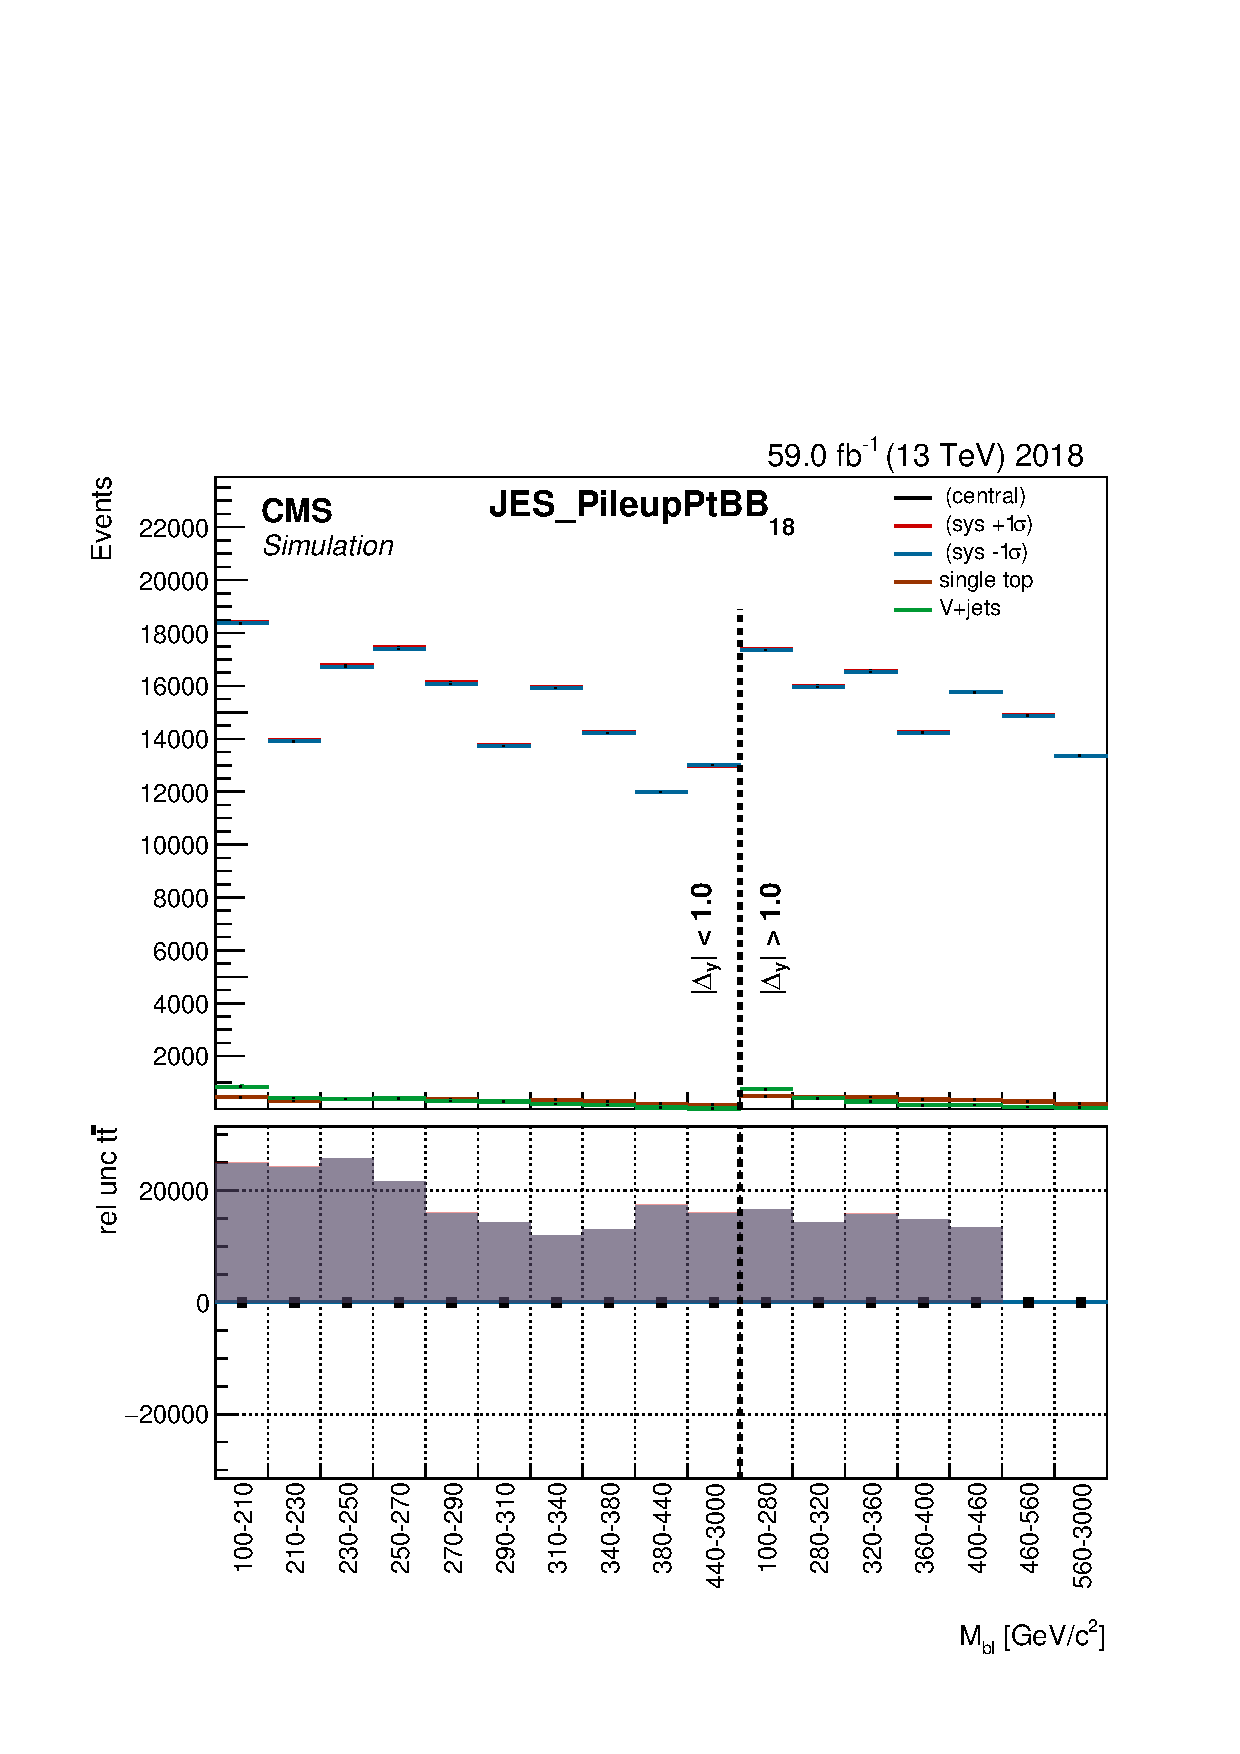
\includegraphics[width=.35\linewidth]{templates/JES_PileupPtBB_18}
\caption{JES\_PileupPtBB templates}
\label{fig:JES-PileupPtBB_template}
\end{figure}

\begin{figure} \centering
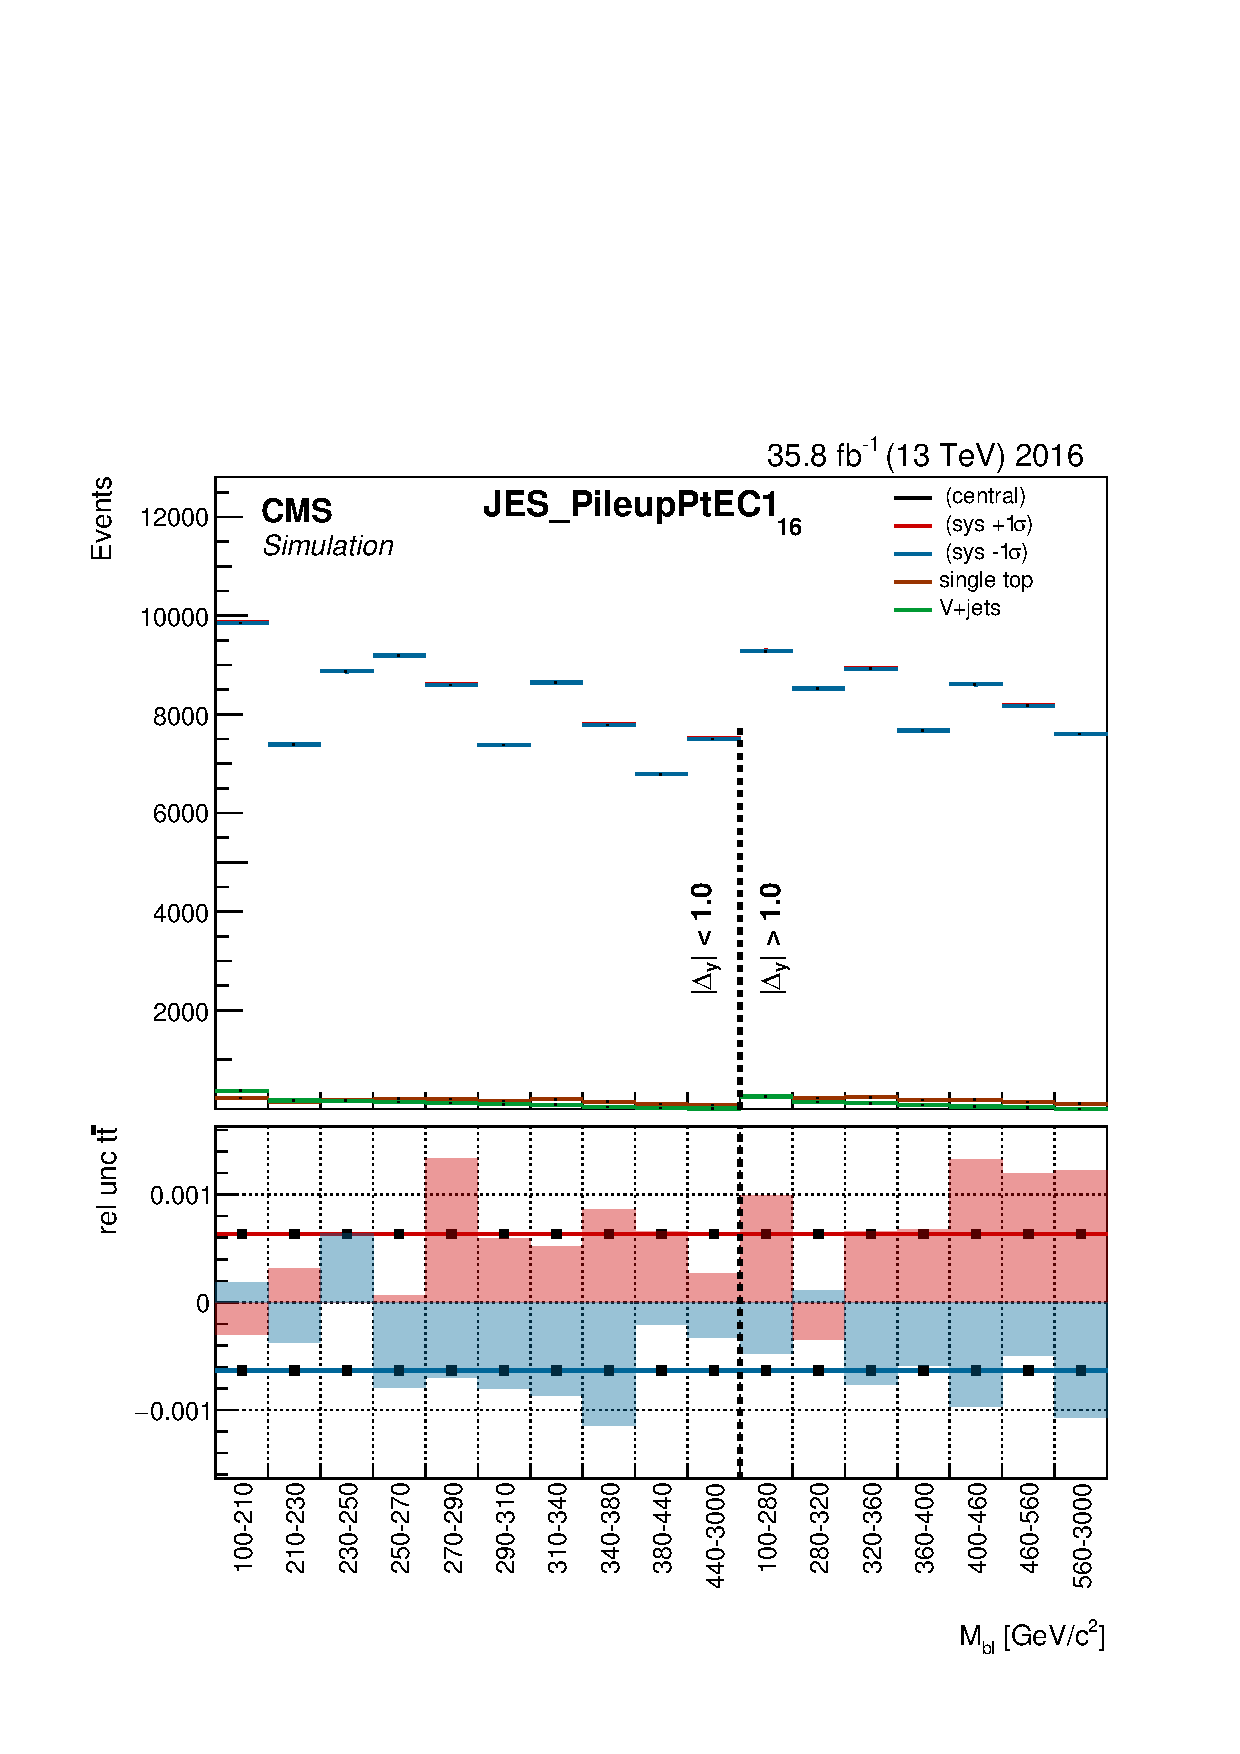
\includegraphics[width=.35\linewidth]{templates/JES_PileupPtEC1_16}\hskip-.5cm
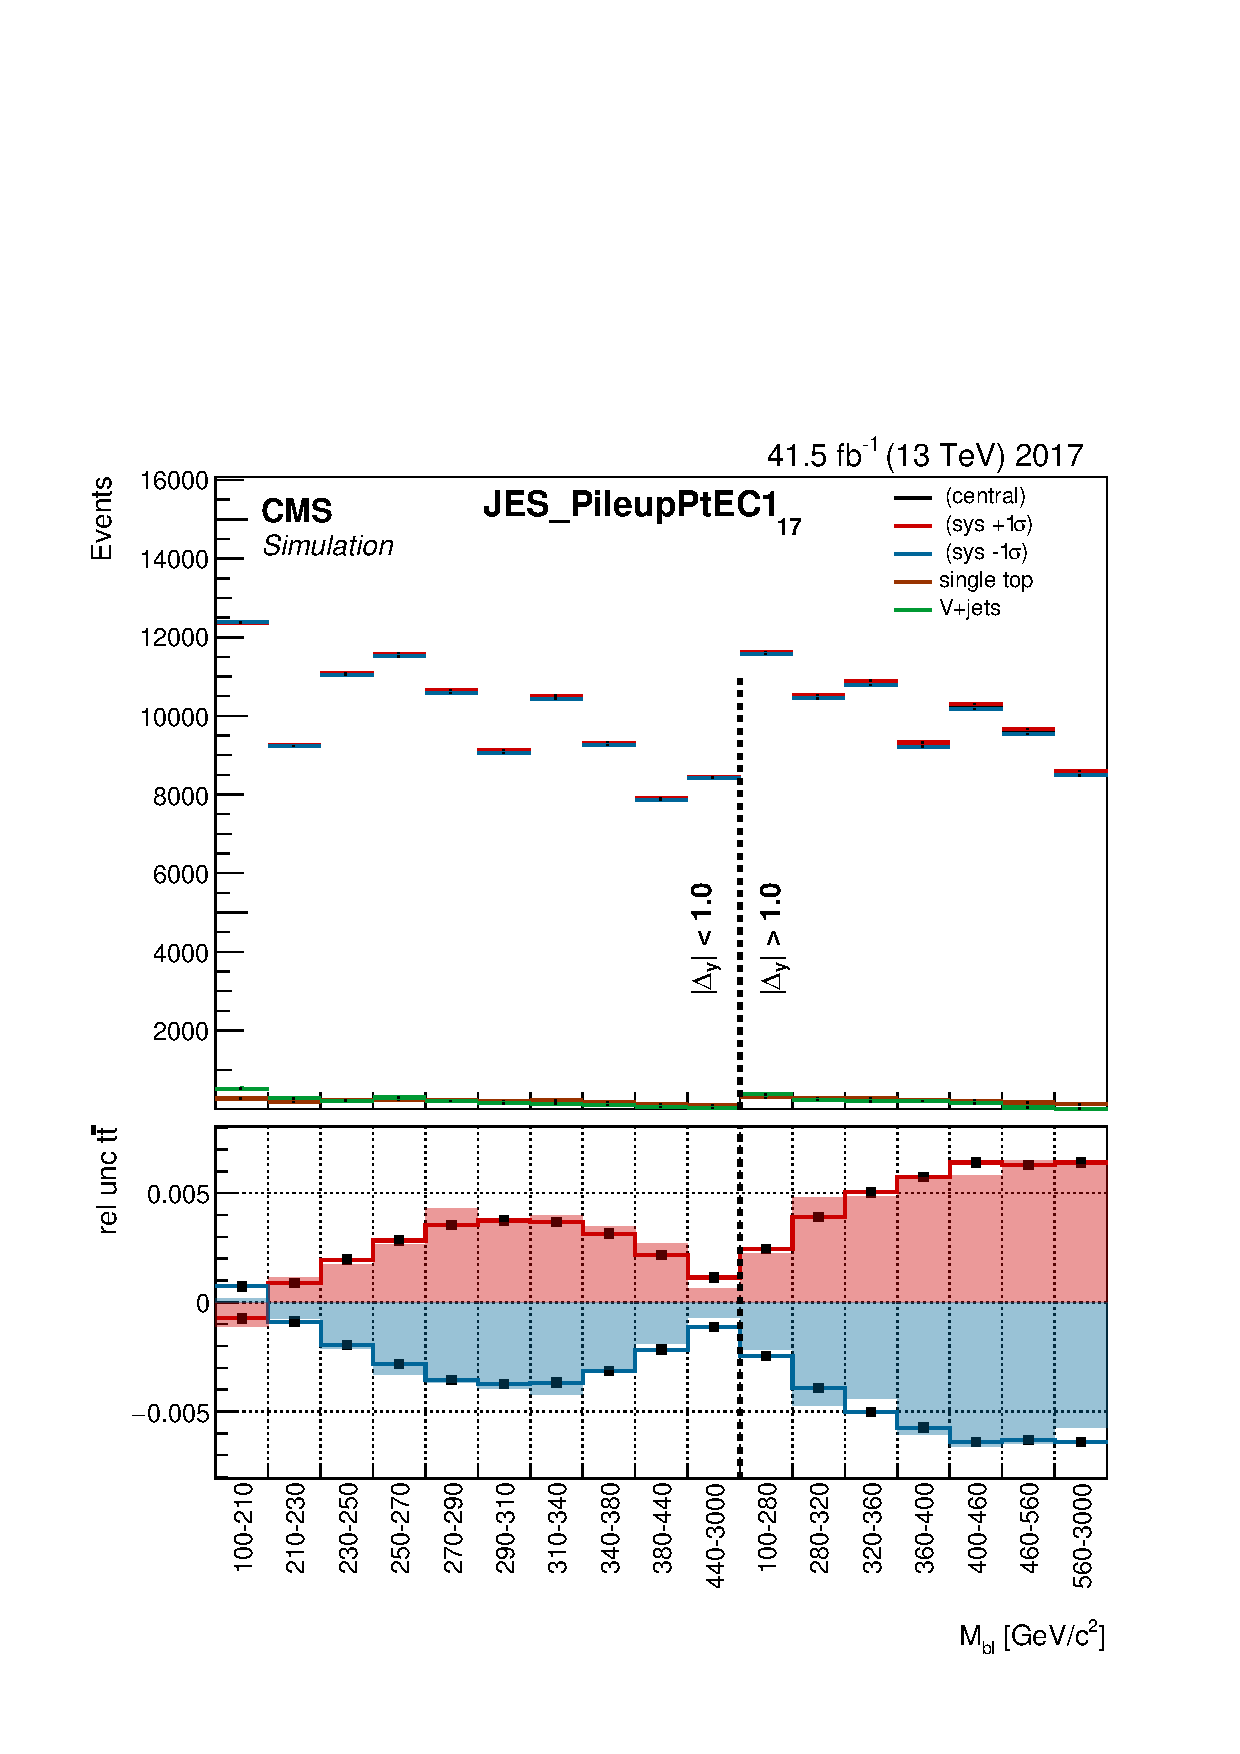
\includegraphics[width=.35\linewidth]{templates/JES_PileupPtEC1_17}\hskip-.5cm
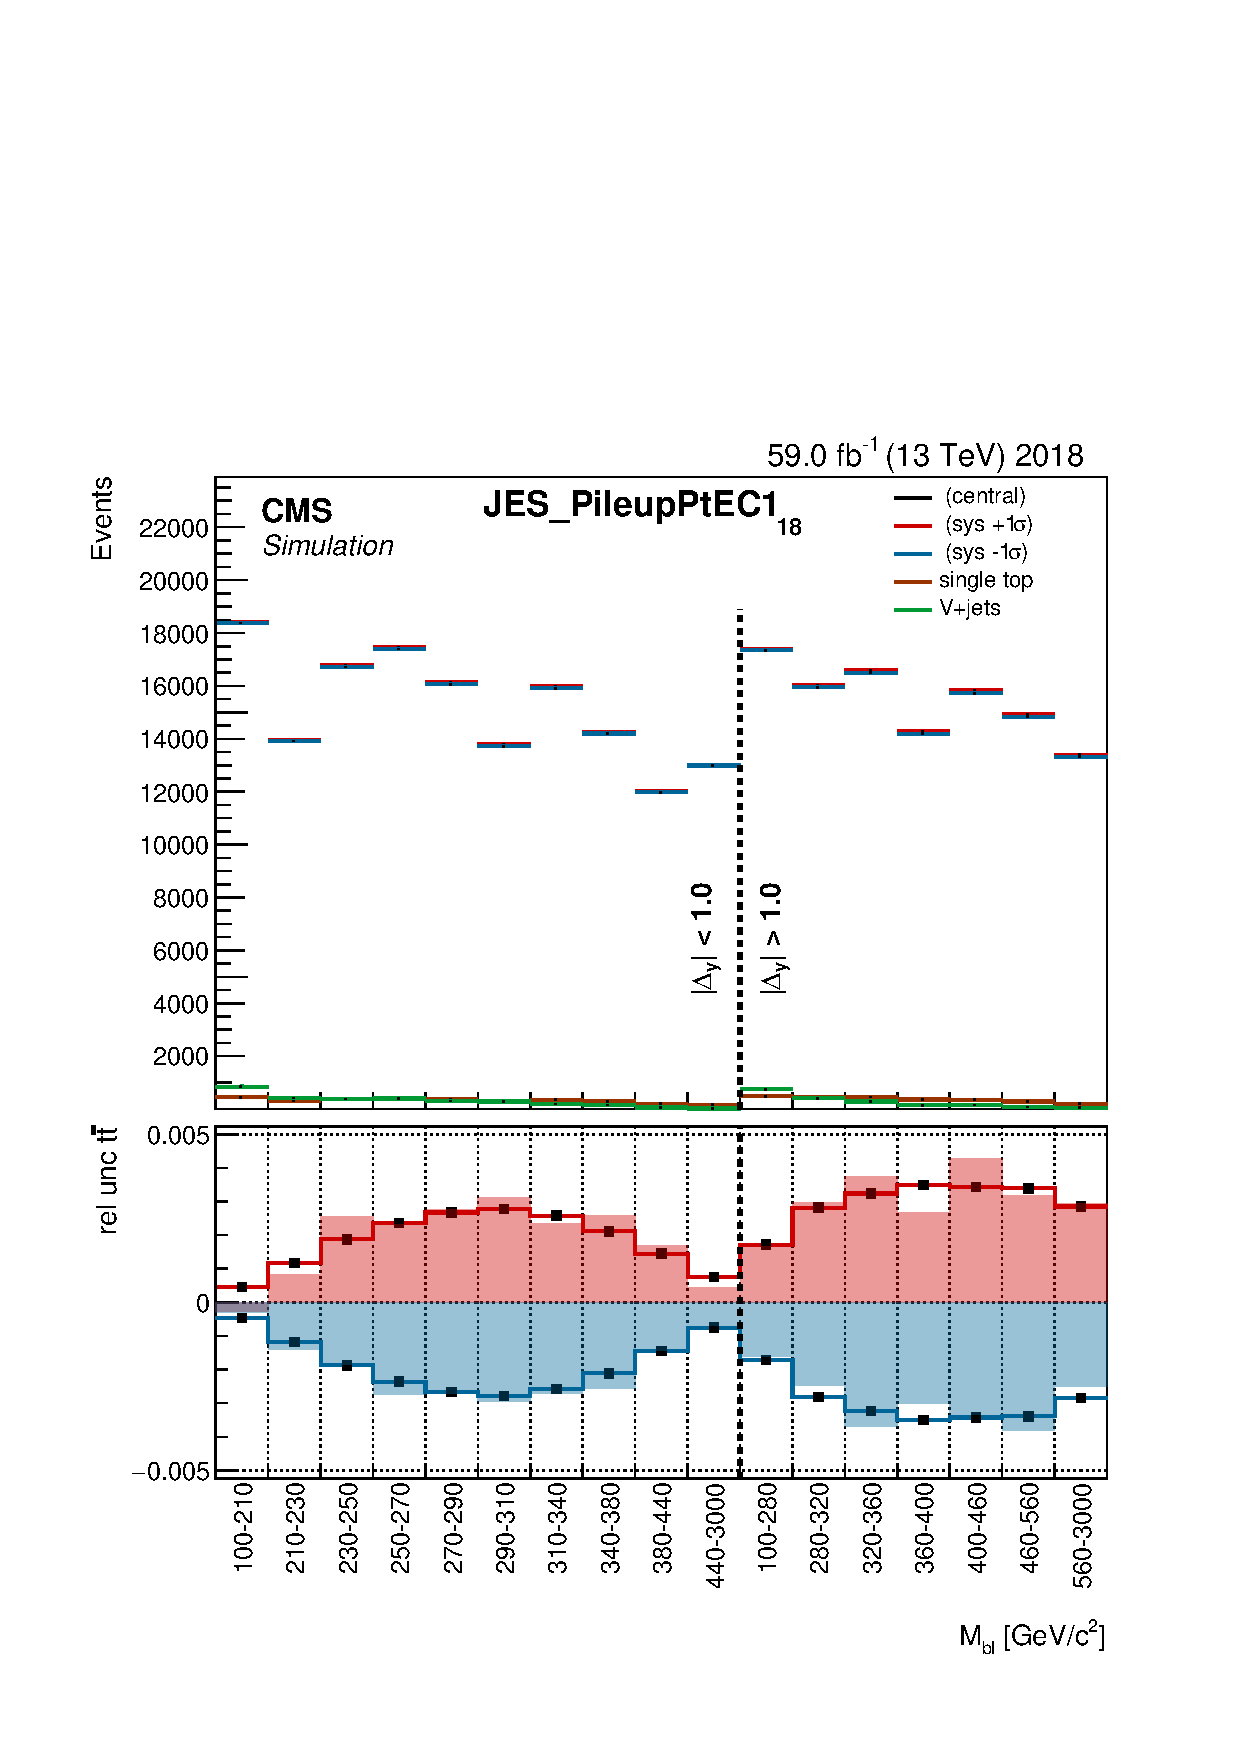
\includegraphics[width=.35\linewidth]{templates/JES_PileupPtEC1_18}
\caption{JES\_PileupPtEC1 templates}
\label{fig:JES-PileupPtEC1_template}
\end{figure}

\begin{figure} \centering
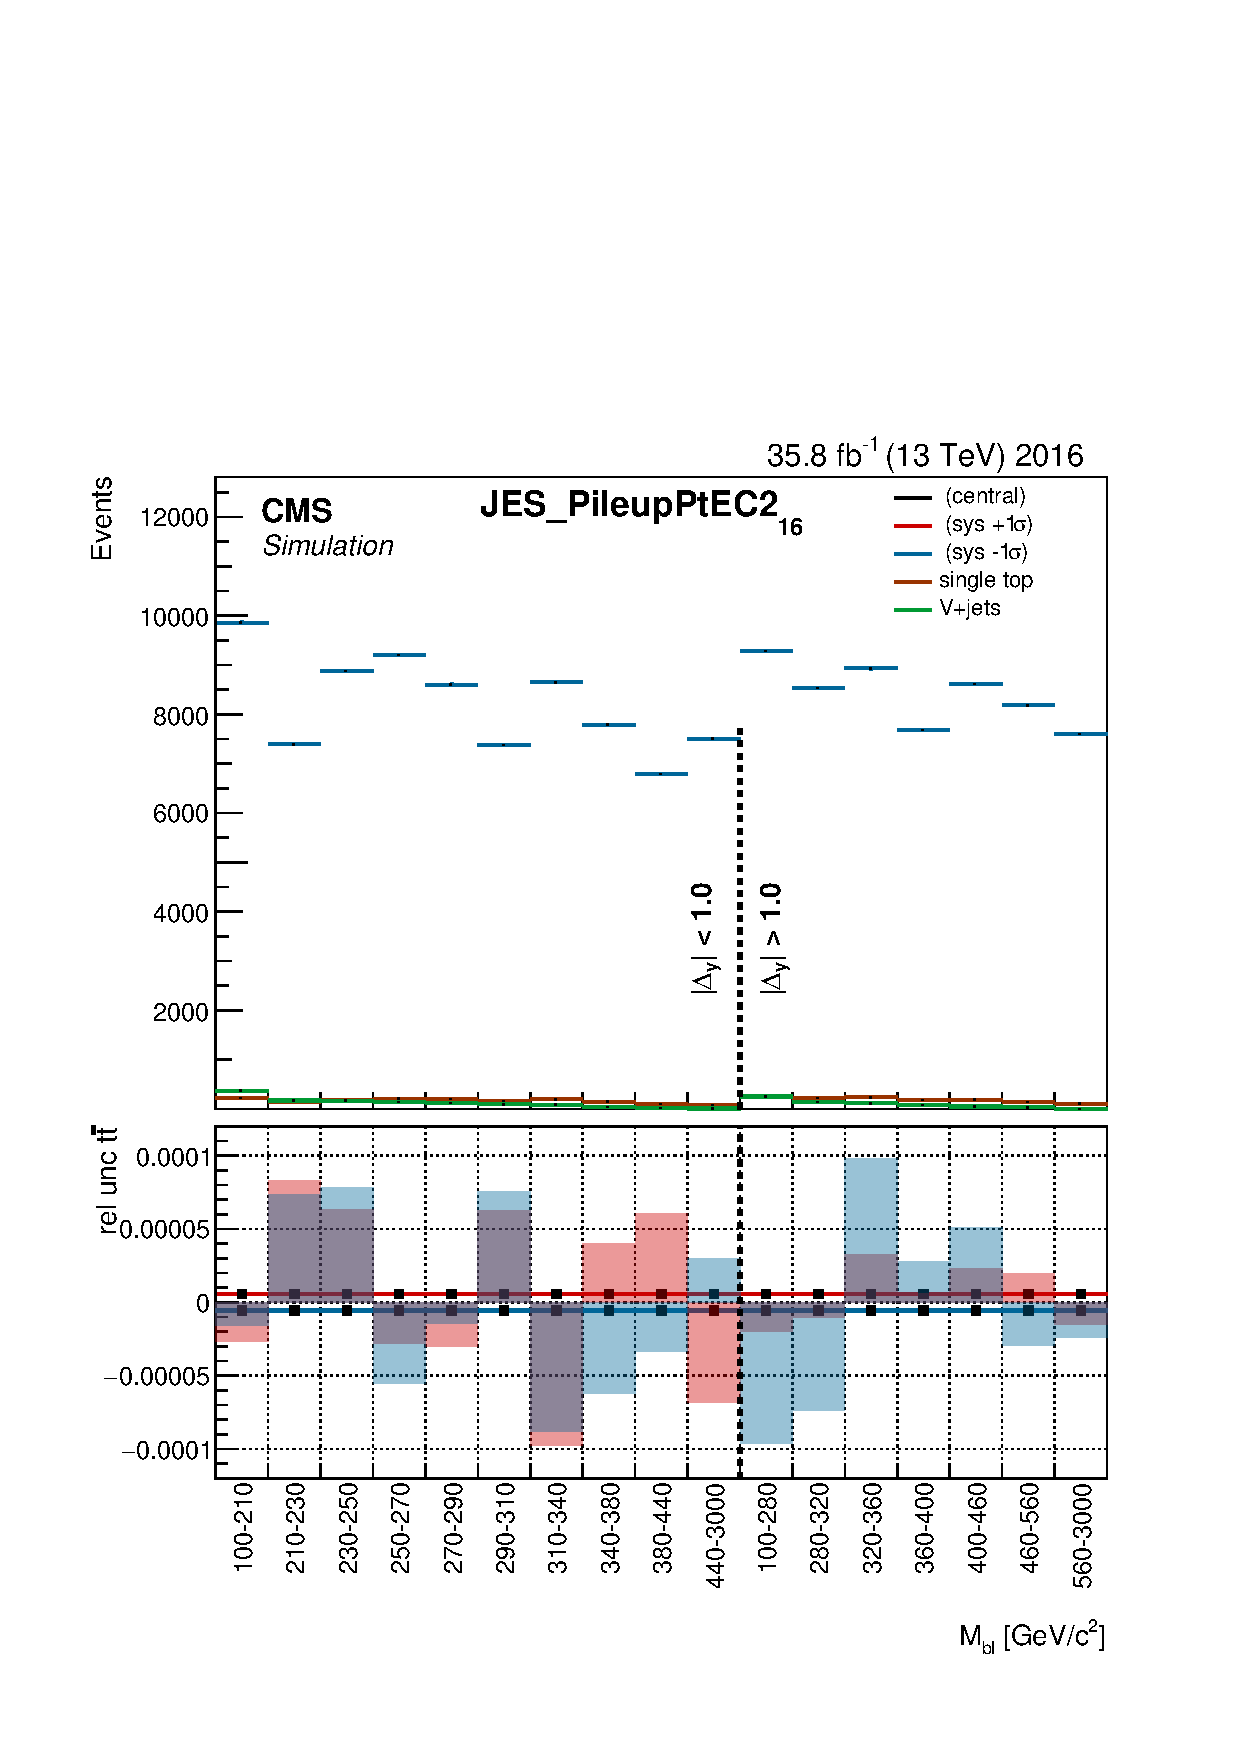
\includegraphics[width=.35\linewidth]{templates/JES_PileupPtEC2_16}\hskip-.5cm
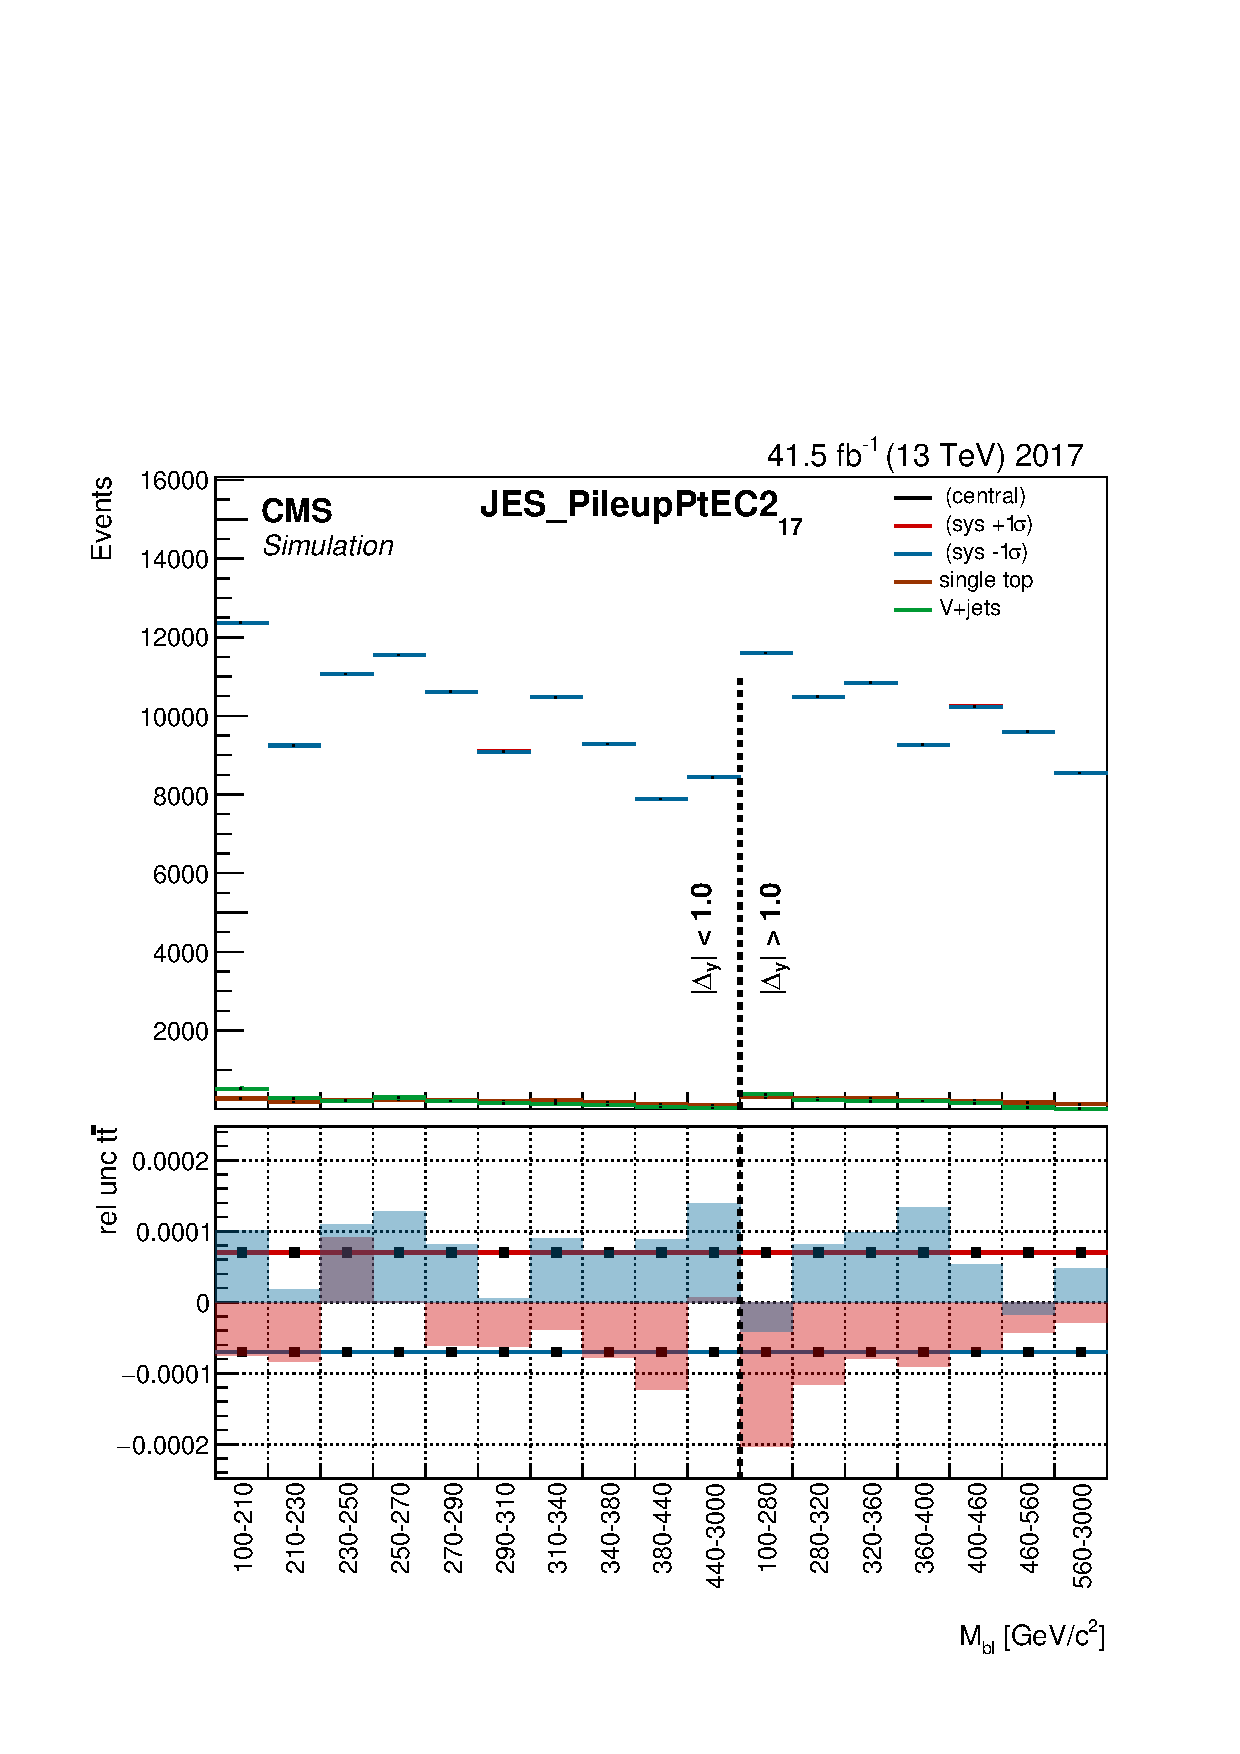
\includegraphics[width=.35\linewidth]{templates/JES_PileupPtEC2_17}\hskip-.5cm
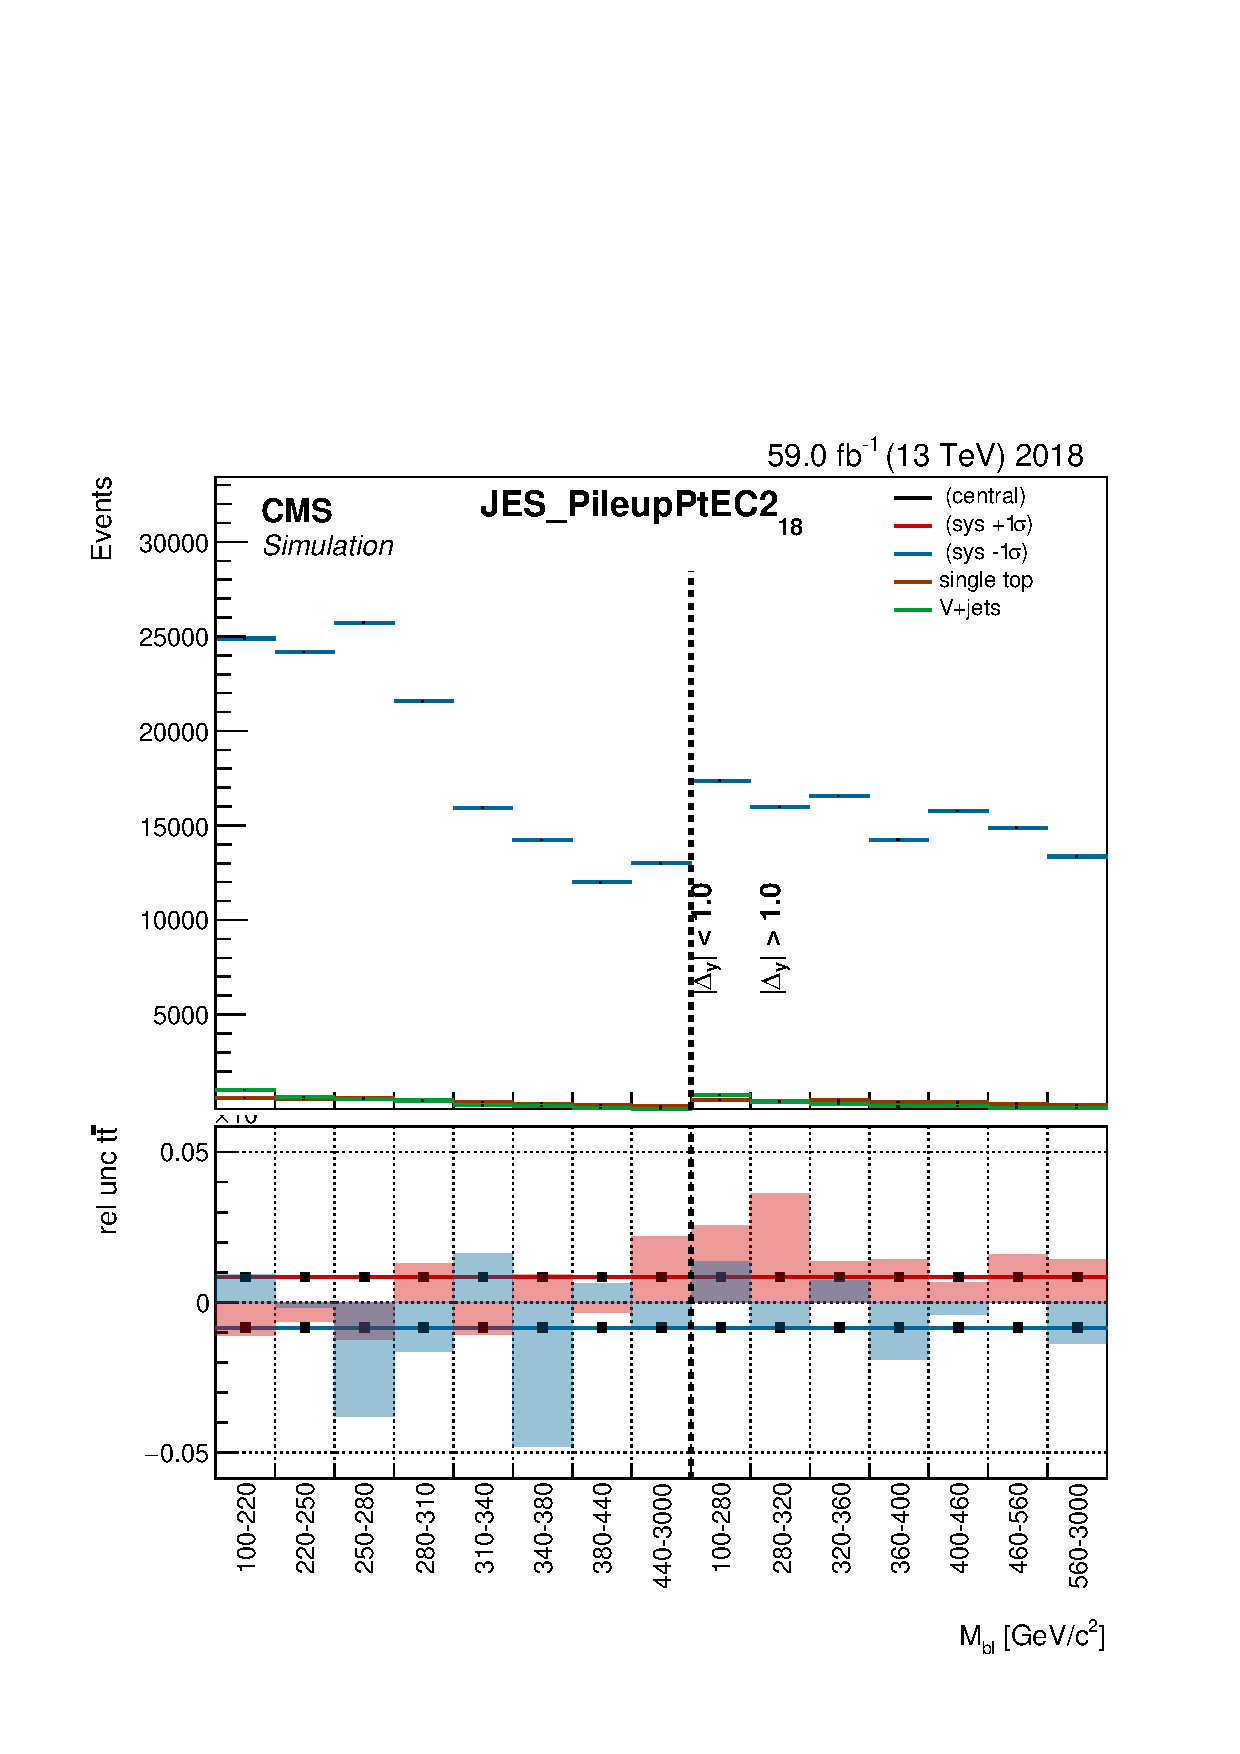
\includegraphics[width=.35\linewidth]{templates/JES_PileupPtEC2_18}
\caption{JES\_PileupPtEC2 templates}
\label{fig:JES-PileupPtEC2_template}
\end{figure}

\begin{figure} \centering
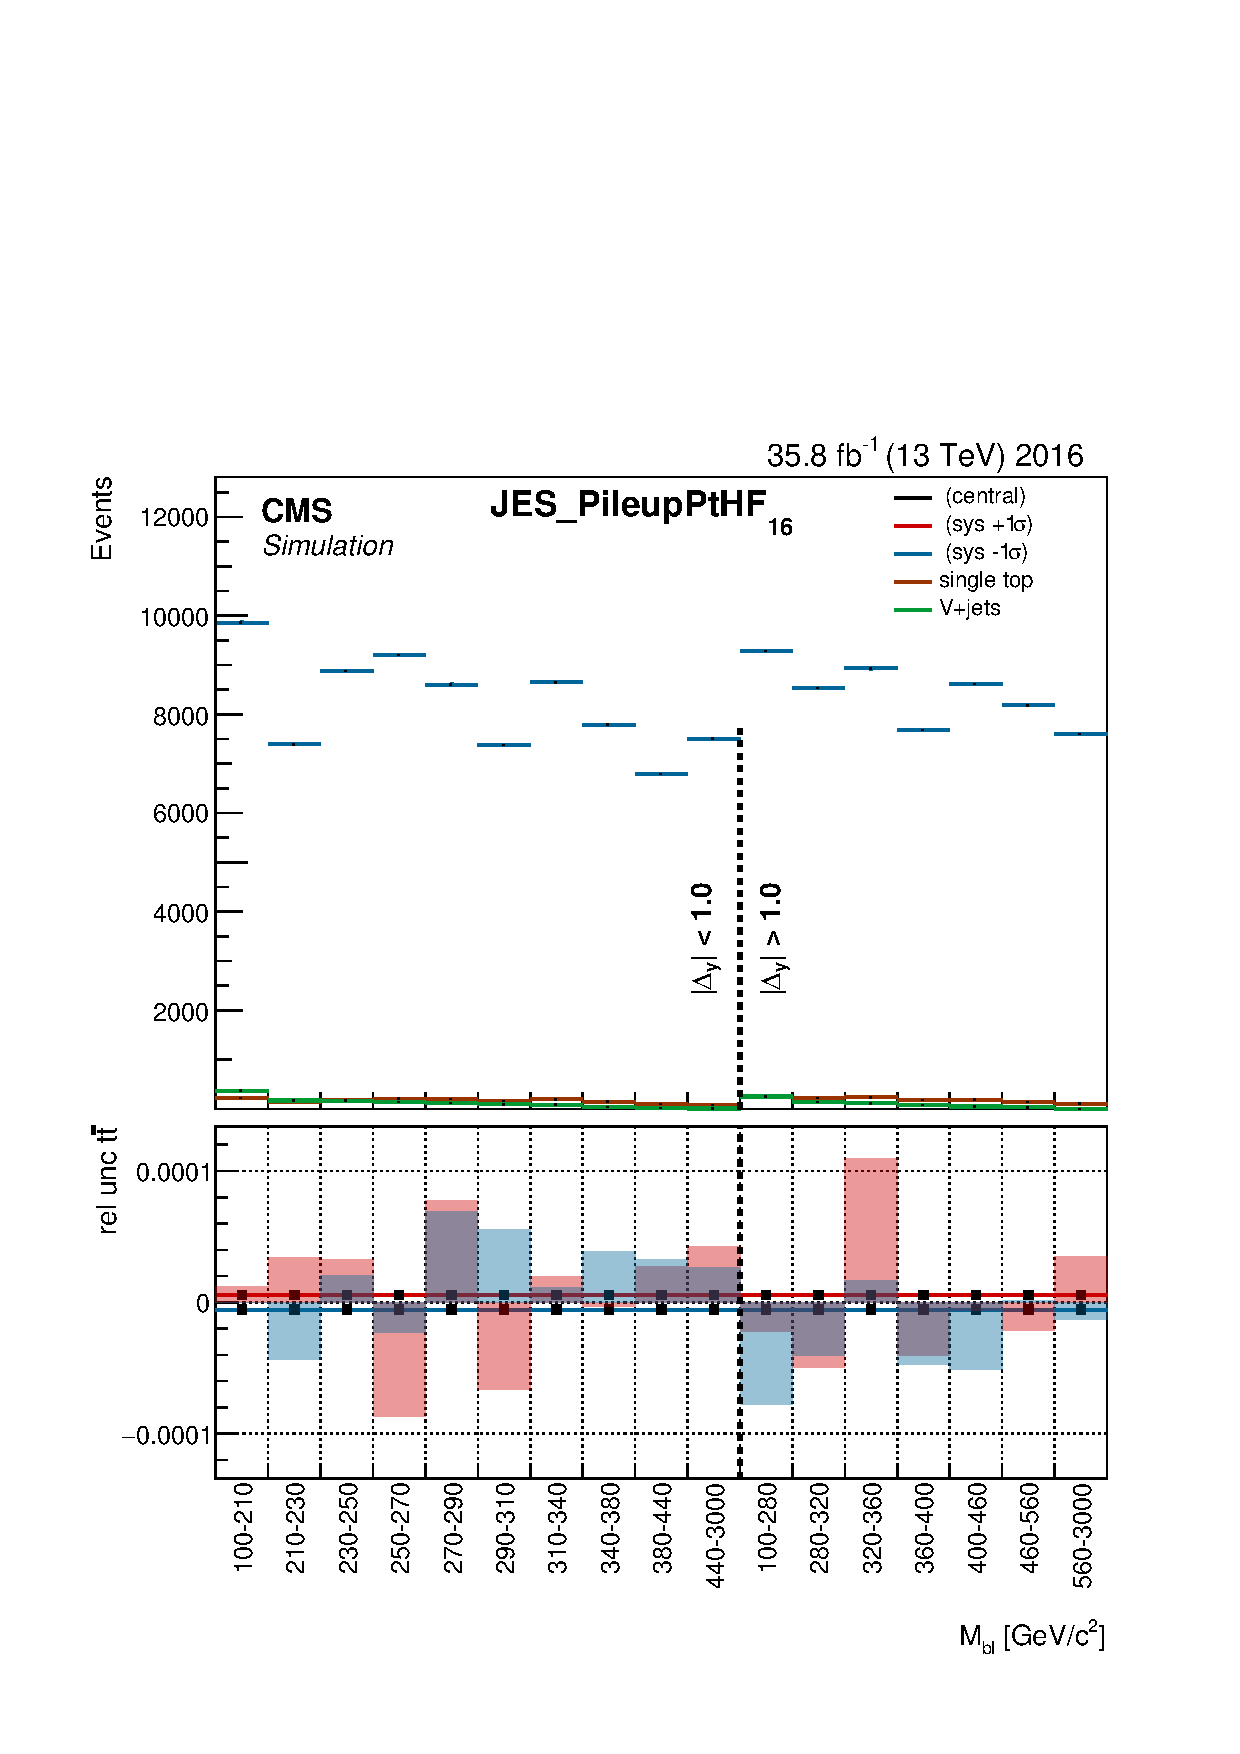
\includegraphics[width=.35\linewidth]{templates/JES_PileupPtHF_16}\hskip-.5cm
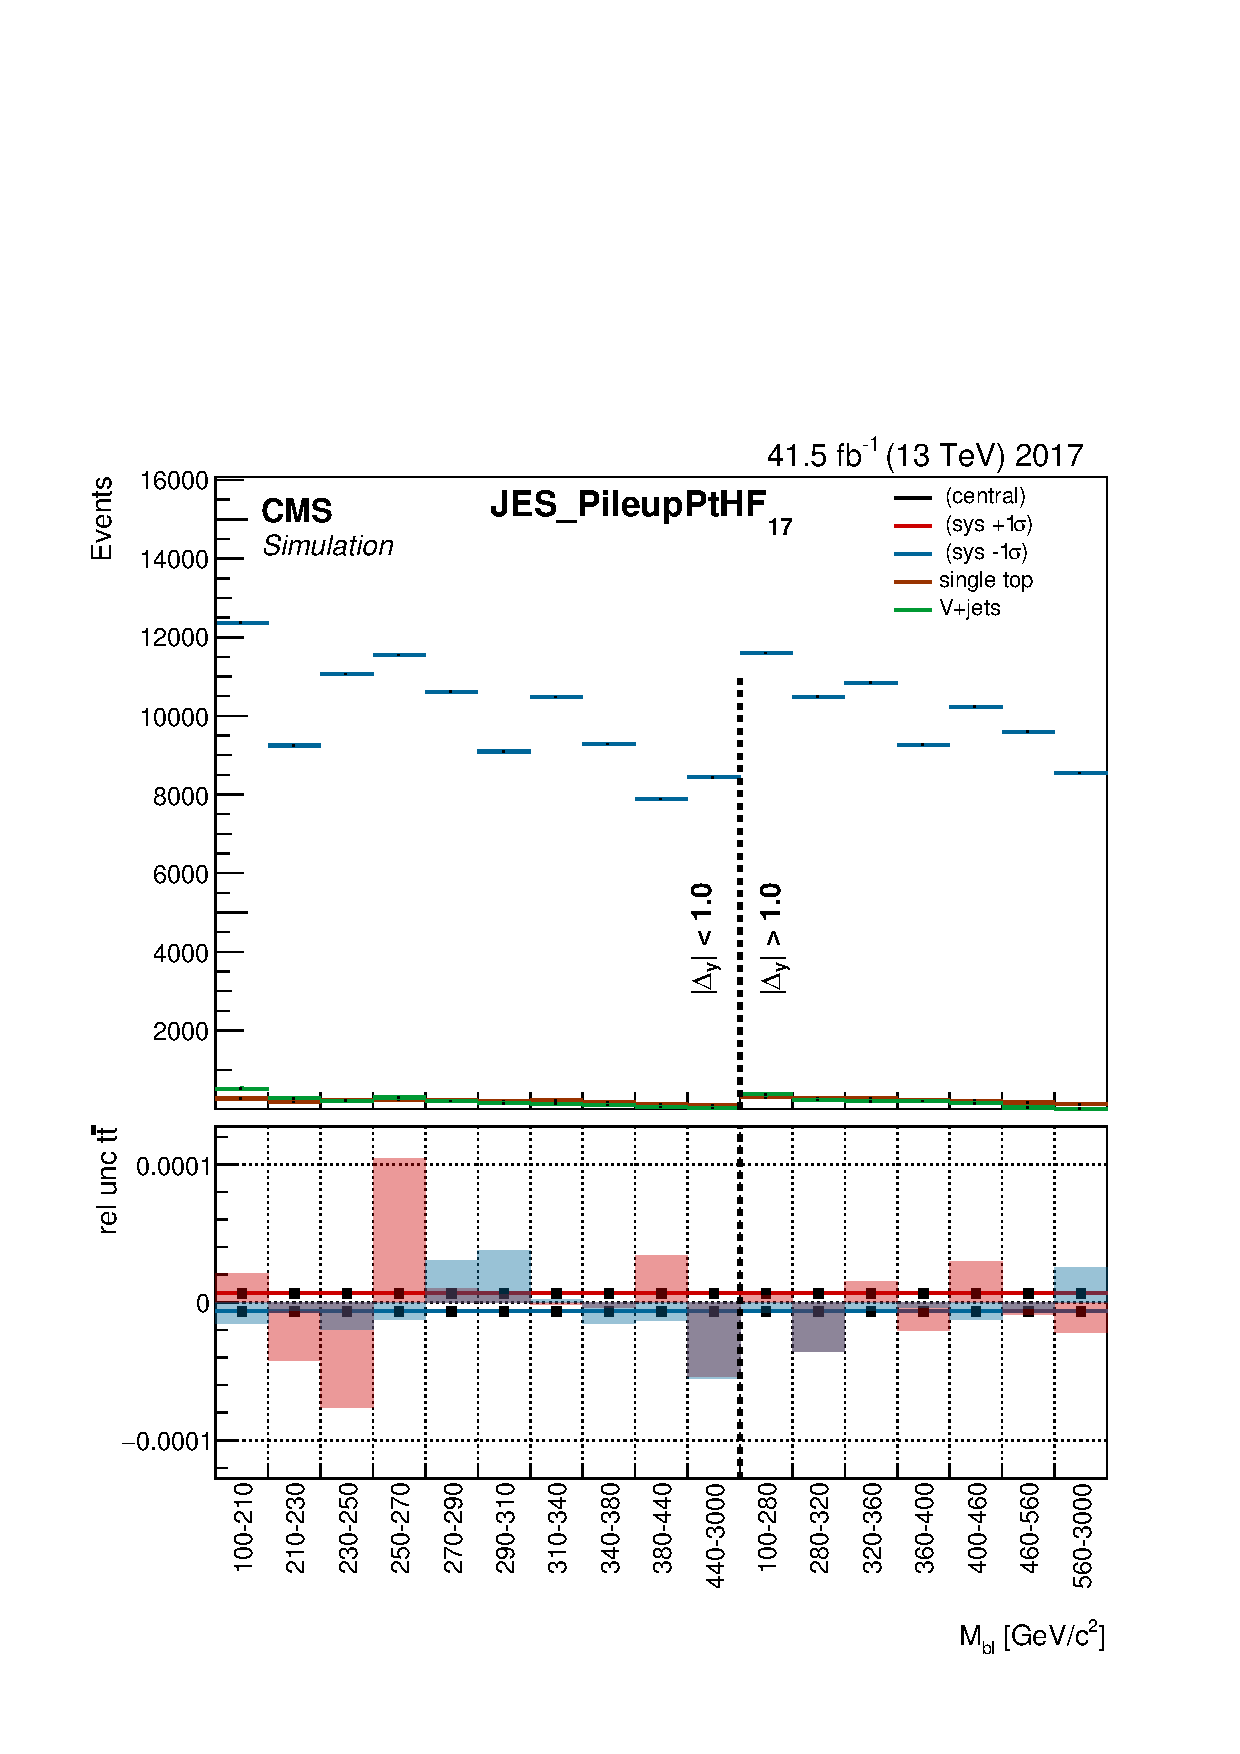
\includegraphics[width=.35\linewidth]{templates/JES_PileupPtHF_17}\hskip-.5cm
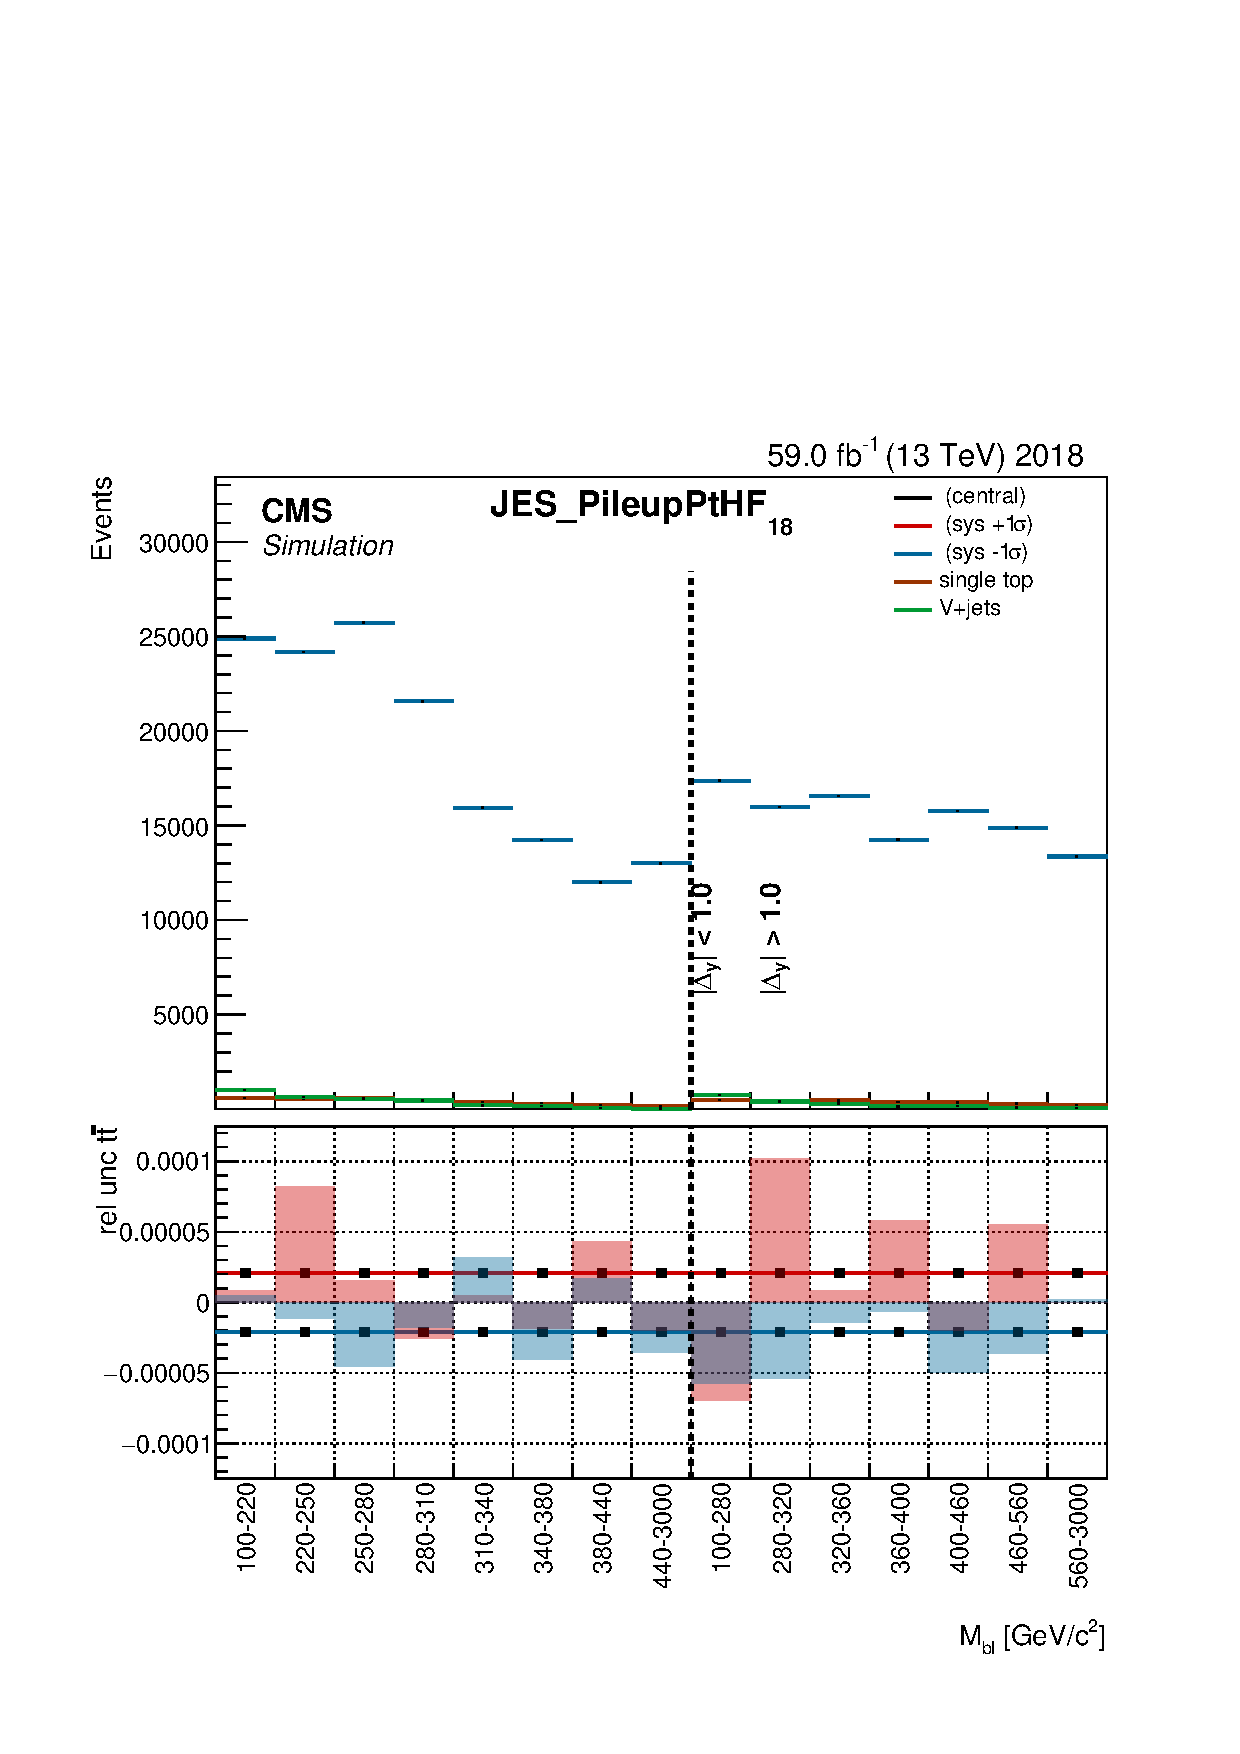
\includegraphics[width=.35\linewidth]{templates/JES_PileupPtHF_18}
\caption{JES\_PileupPtHF templates}
\label{fig:JES-PileupPtHF_template}
\end{figure}

\begin{figure} \centering
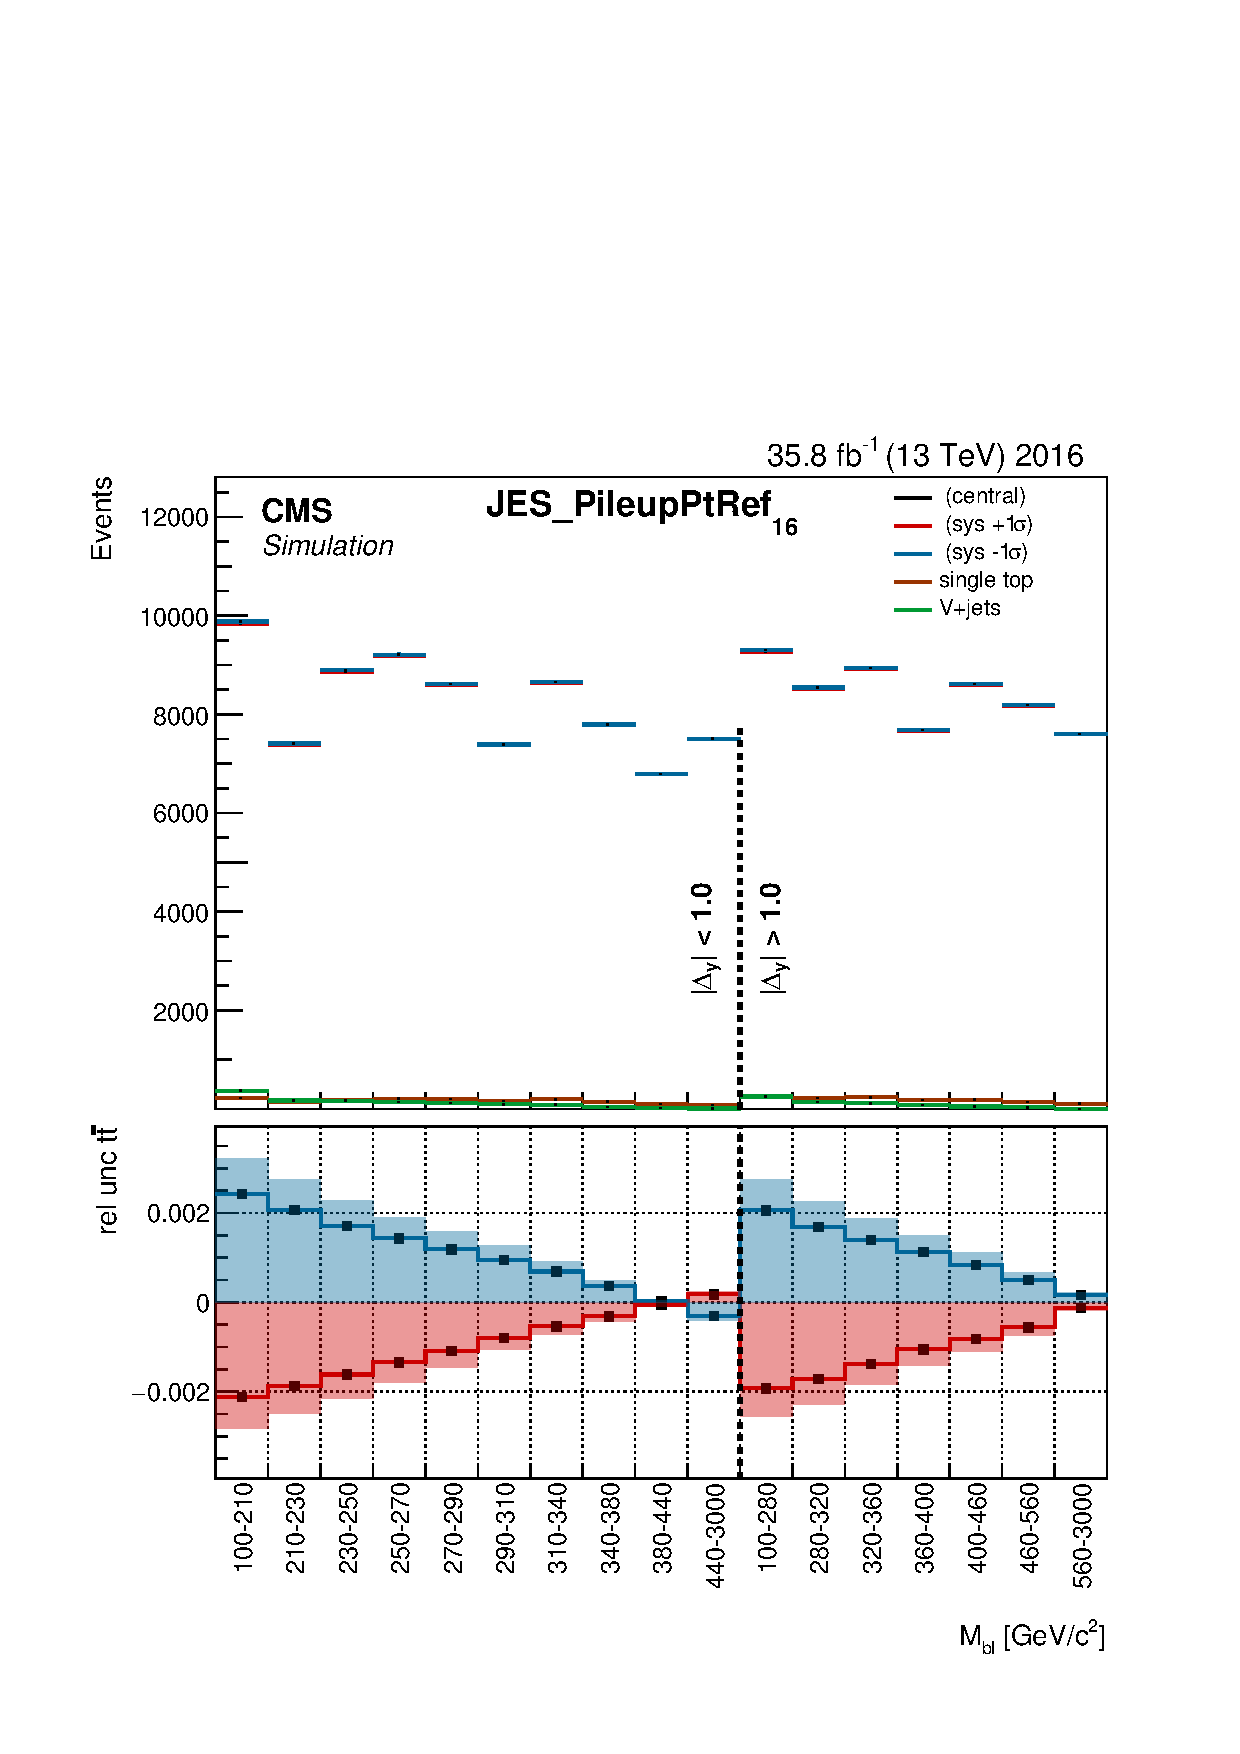
\includegraphics[width=.35\linewidth]{templates/JES_PileupPtRef_16}\hskip-.5cm
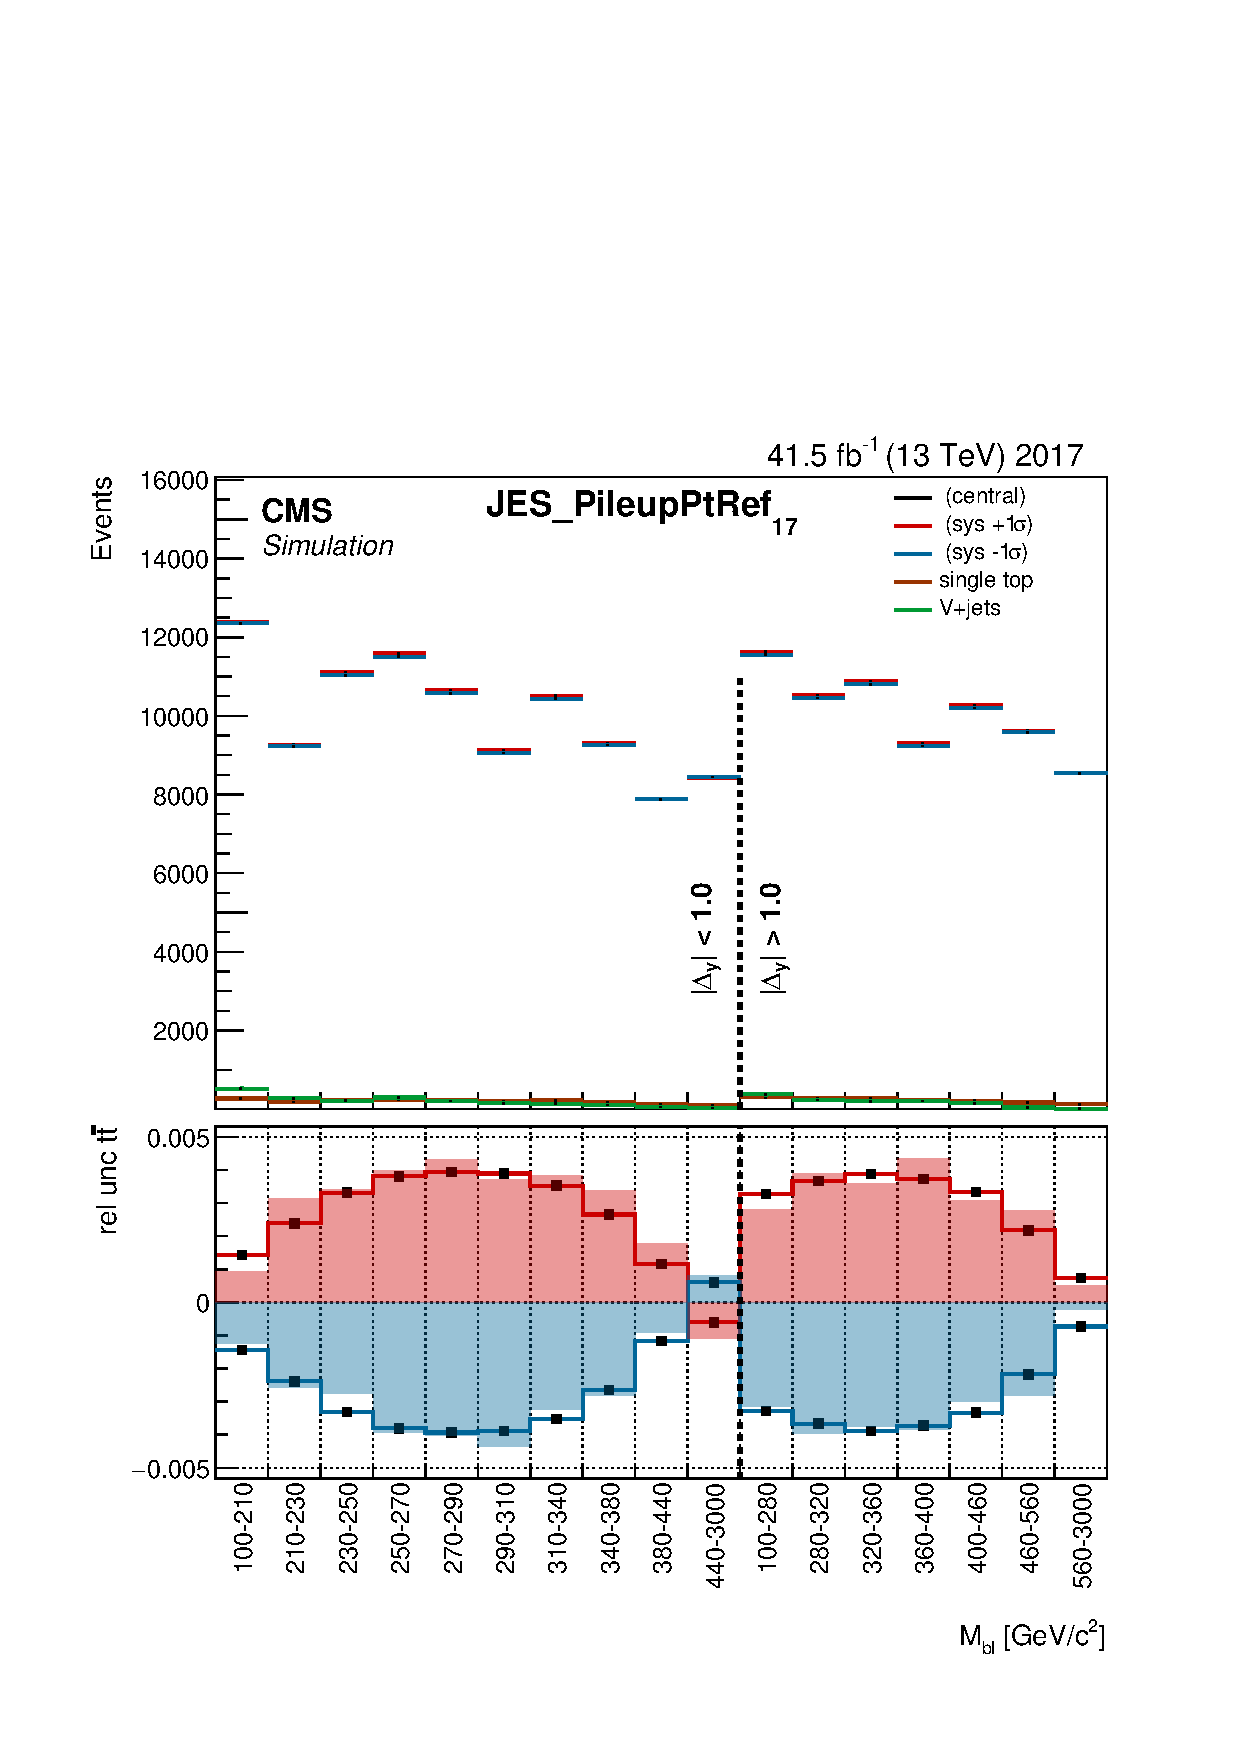
\includegraphics[width=.35\linewidth]{templates/JES_PileupPtRef_17}\hskip-.5cm
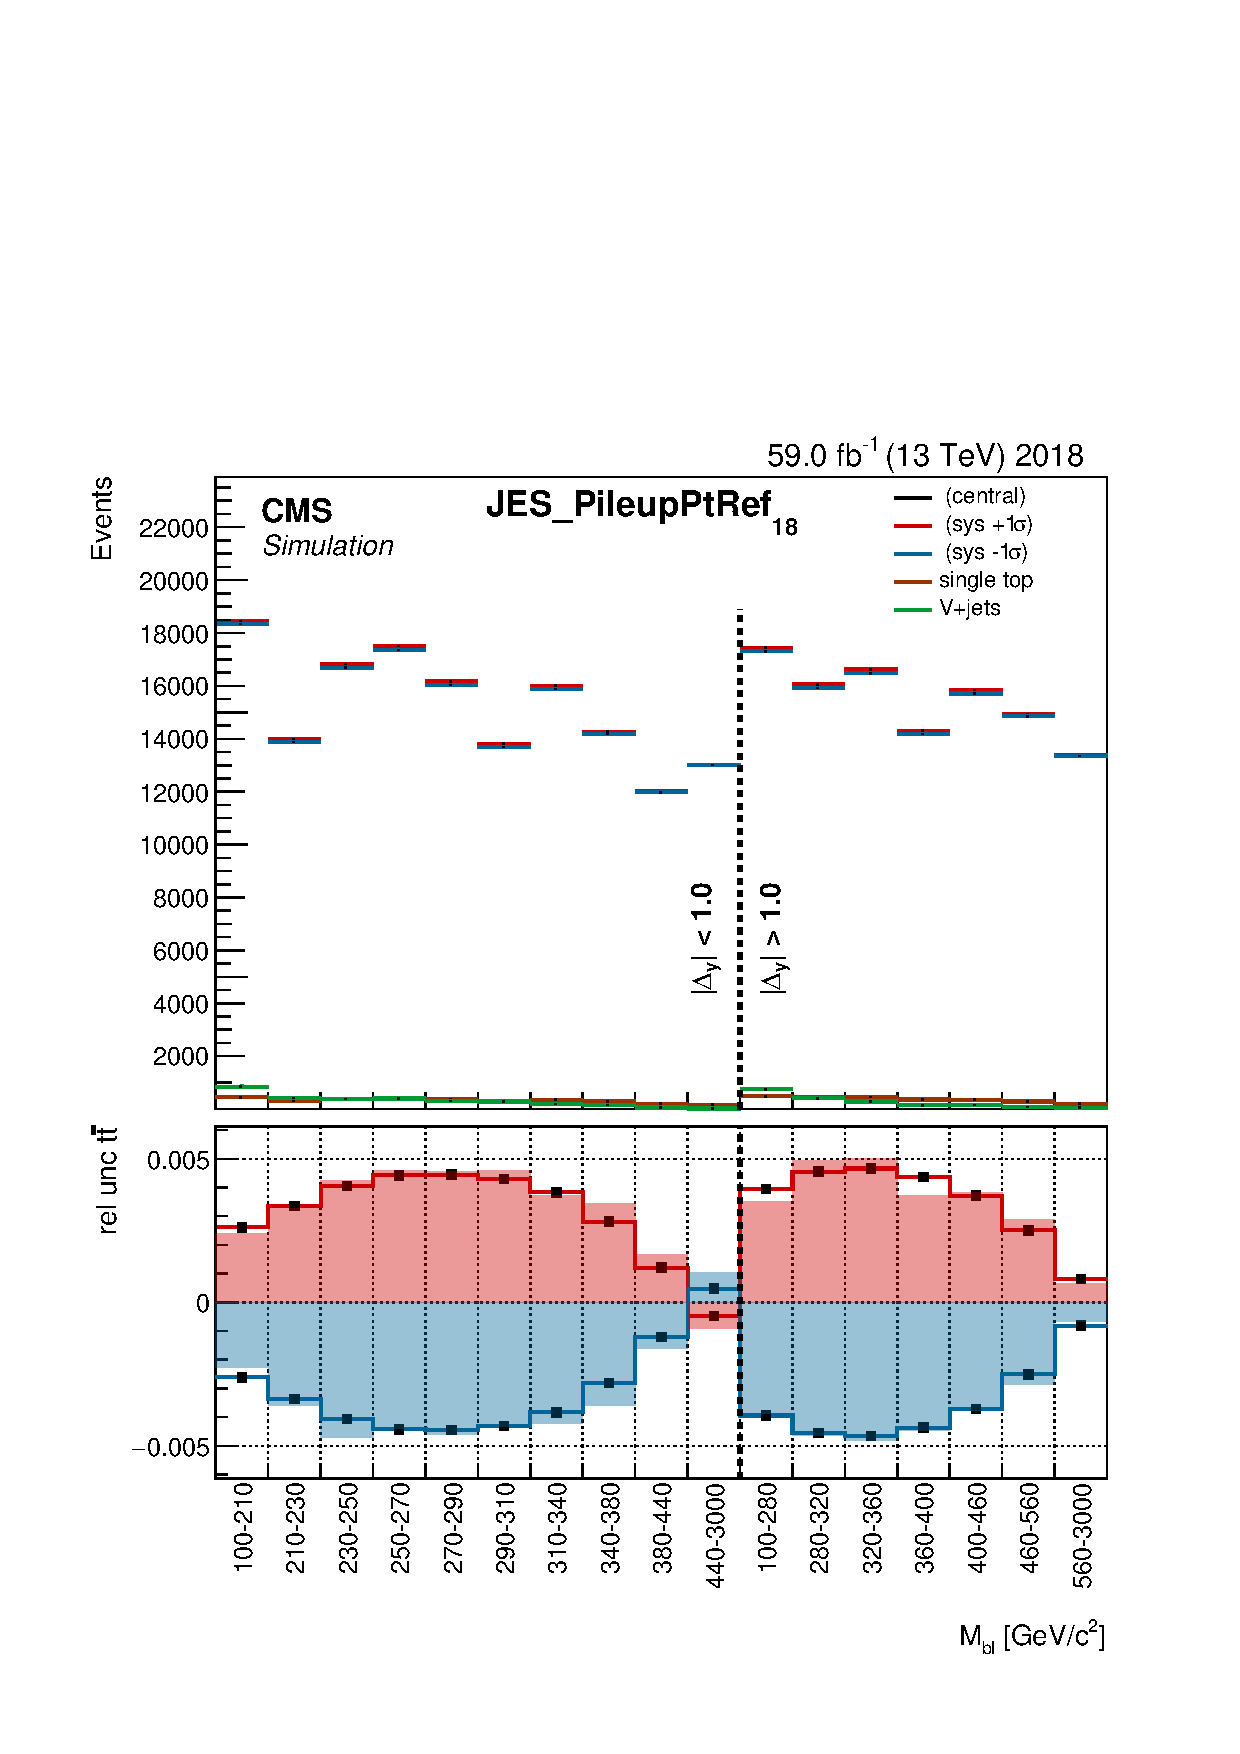
\includegraphics[width=.35\linewidth]{templates/JES_PileupPtRef_18}
\caption{JES\_PileupPtRef templates}
\label{fig:JES-PileupPtRef_template}
\end{figure}

\begin{figure} \centering
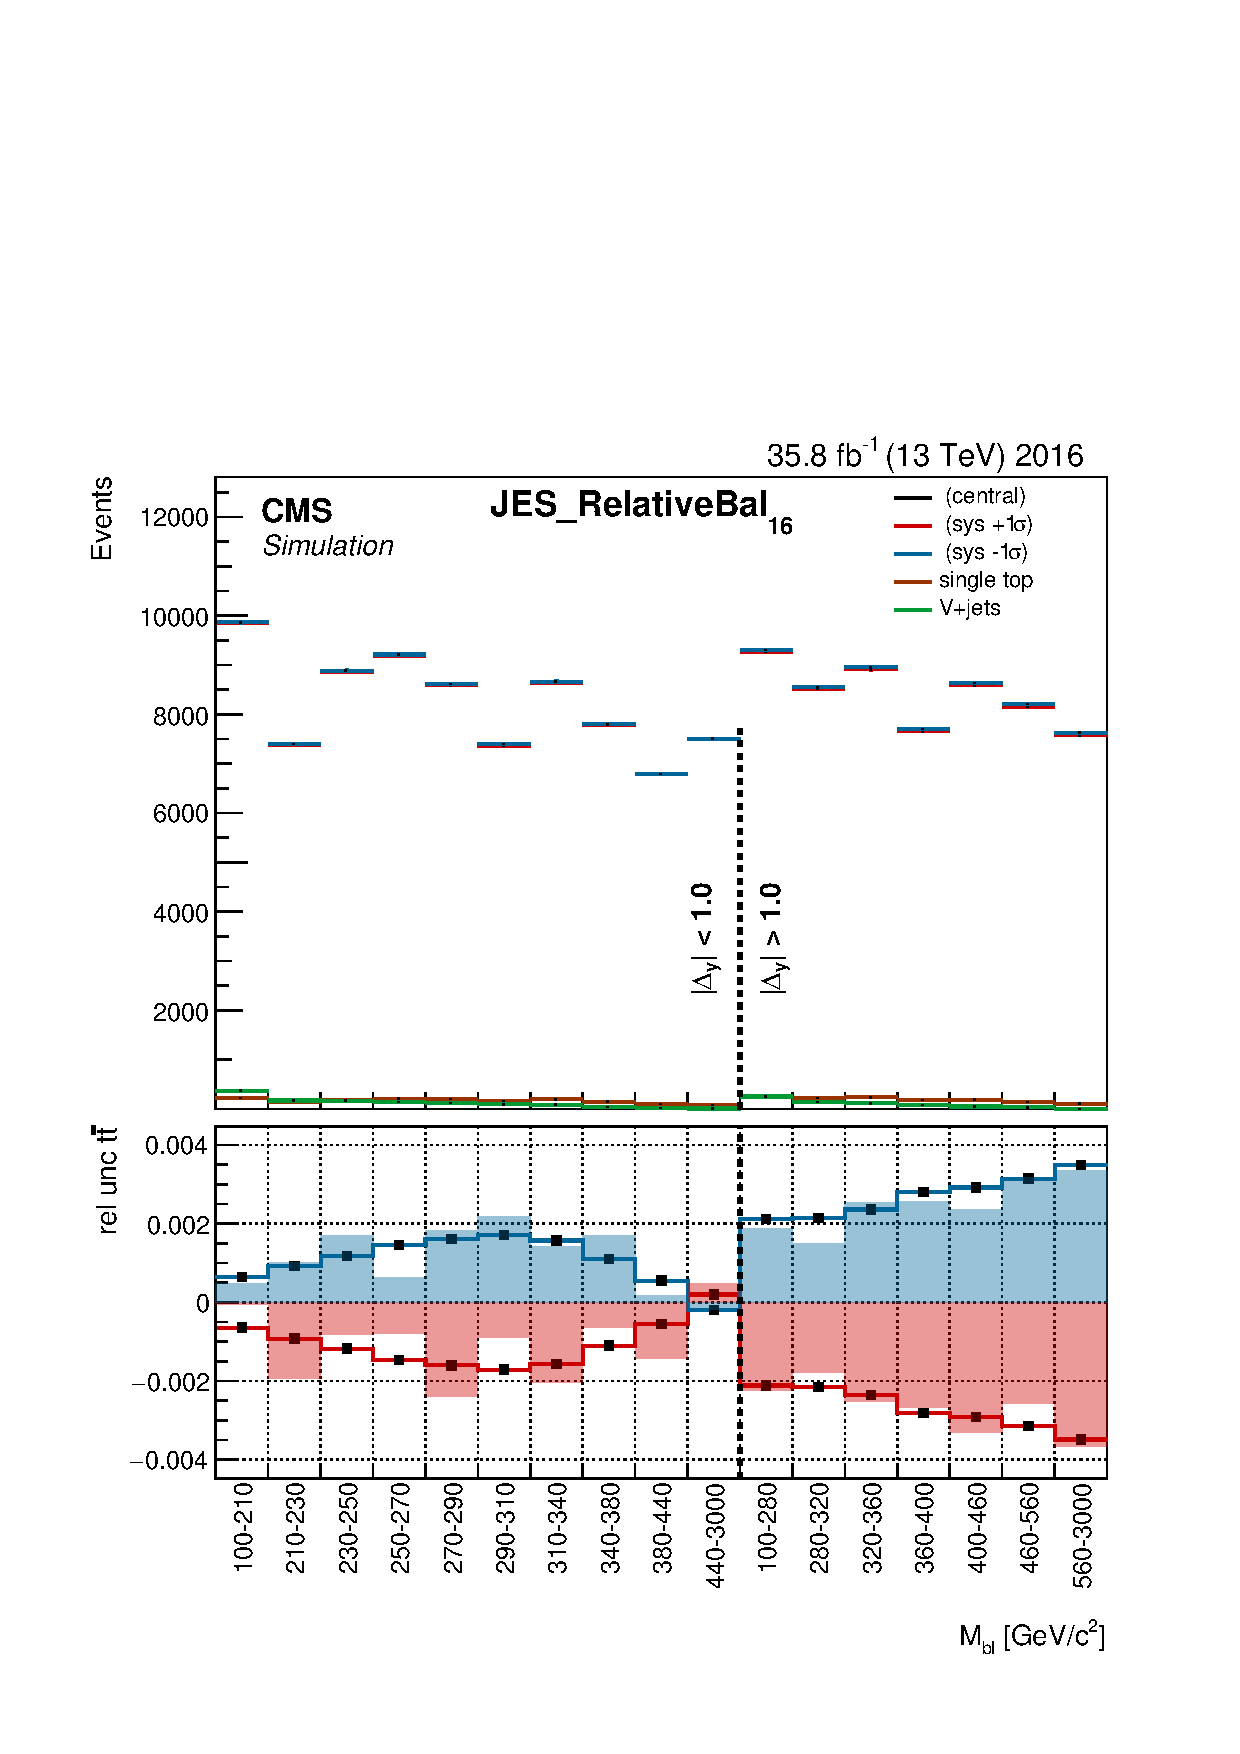
\includegraphics[width=.35\linewidth]{templates/JES_RelativeBal_16}\hskip-.5cm
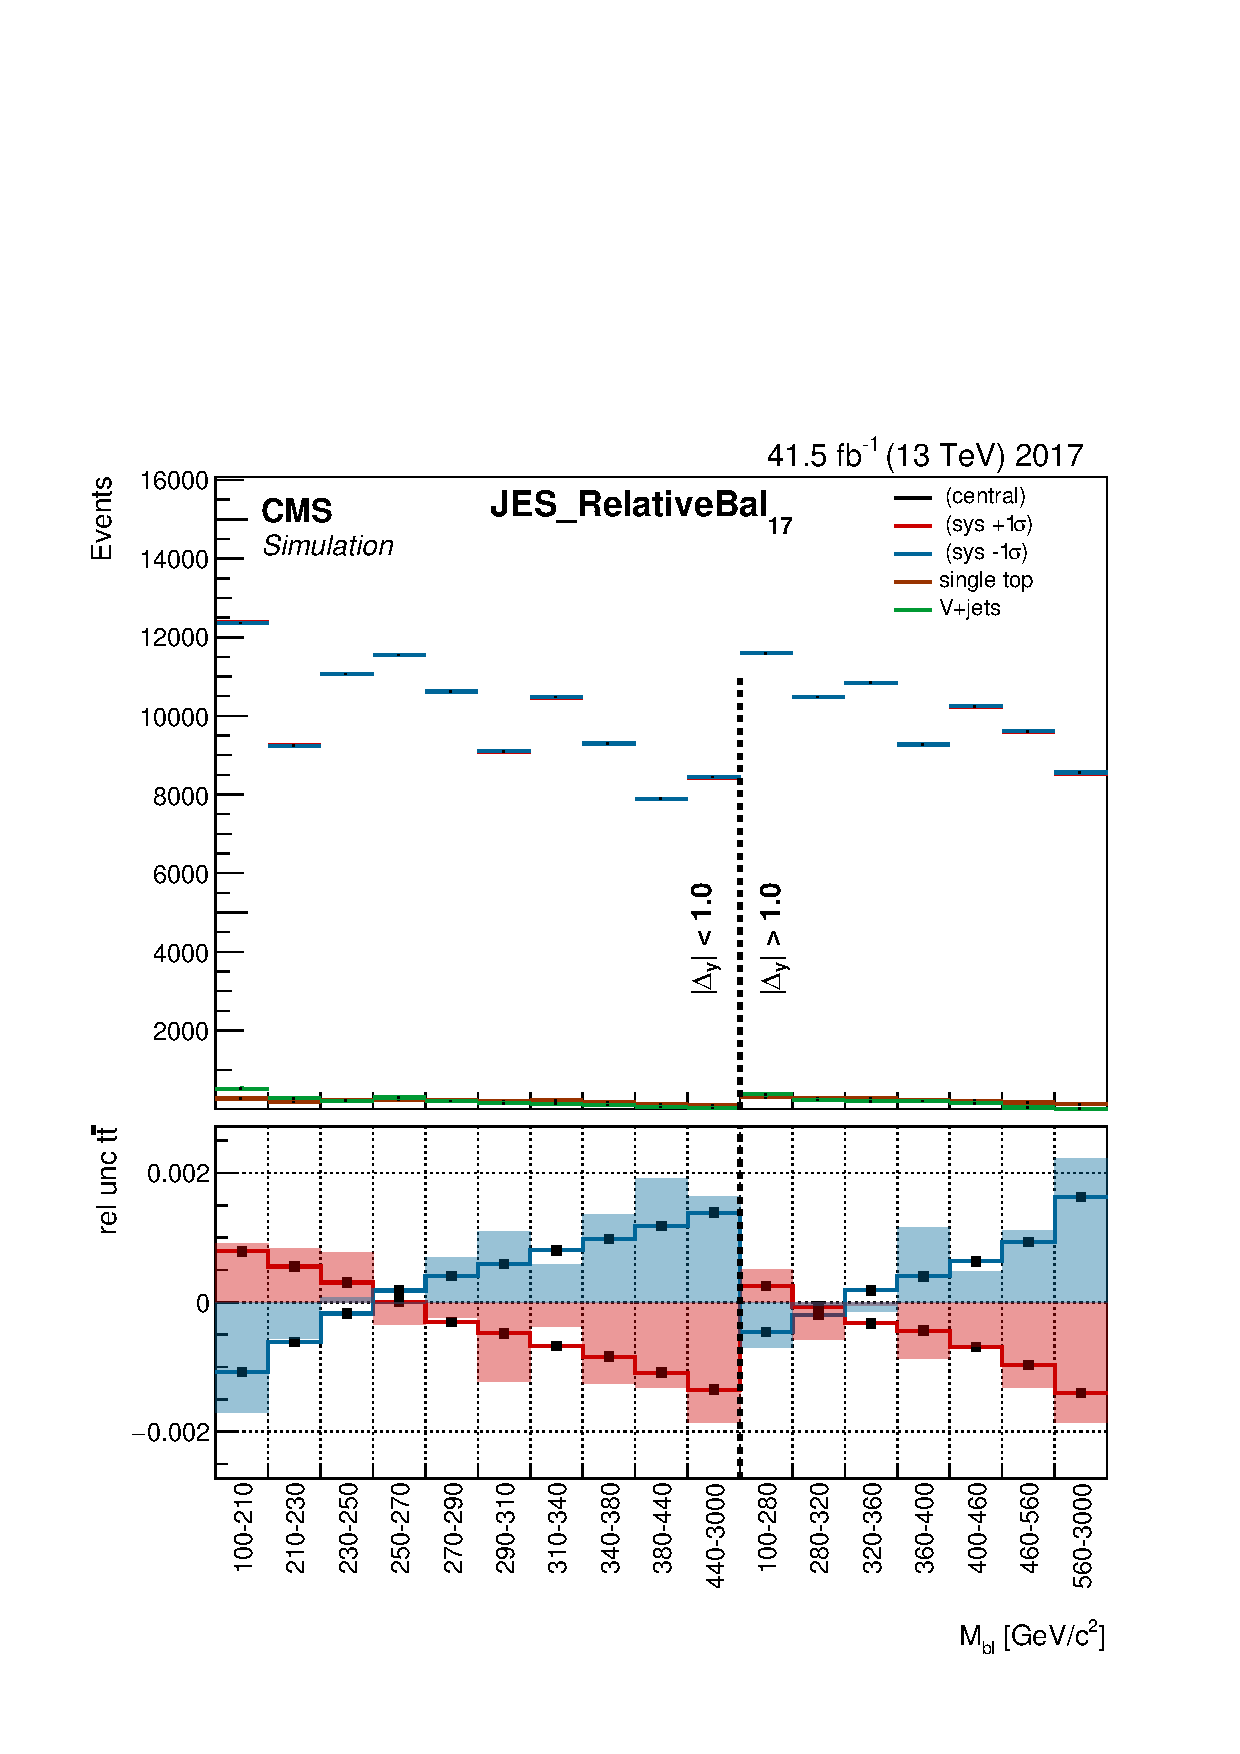
\includegraphics[width=.35\linewidth]{templates/JES_RelativeBal_17}\hskip-.5cm
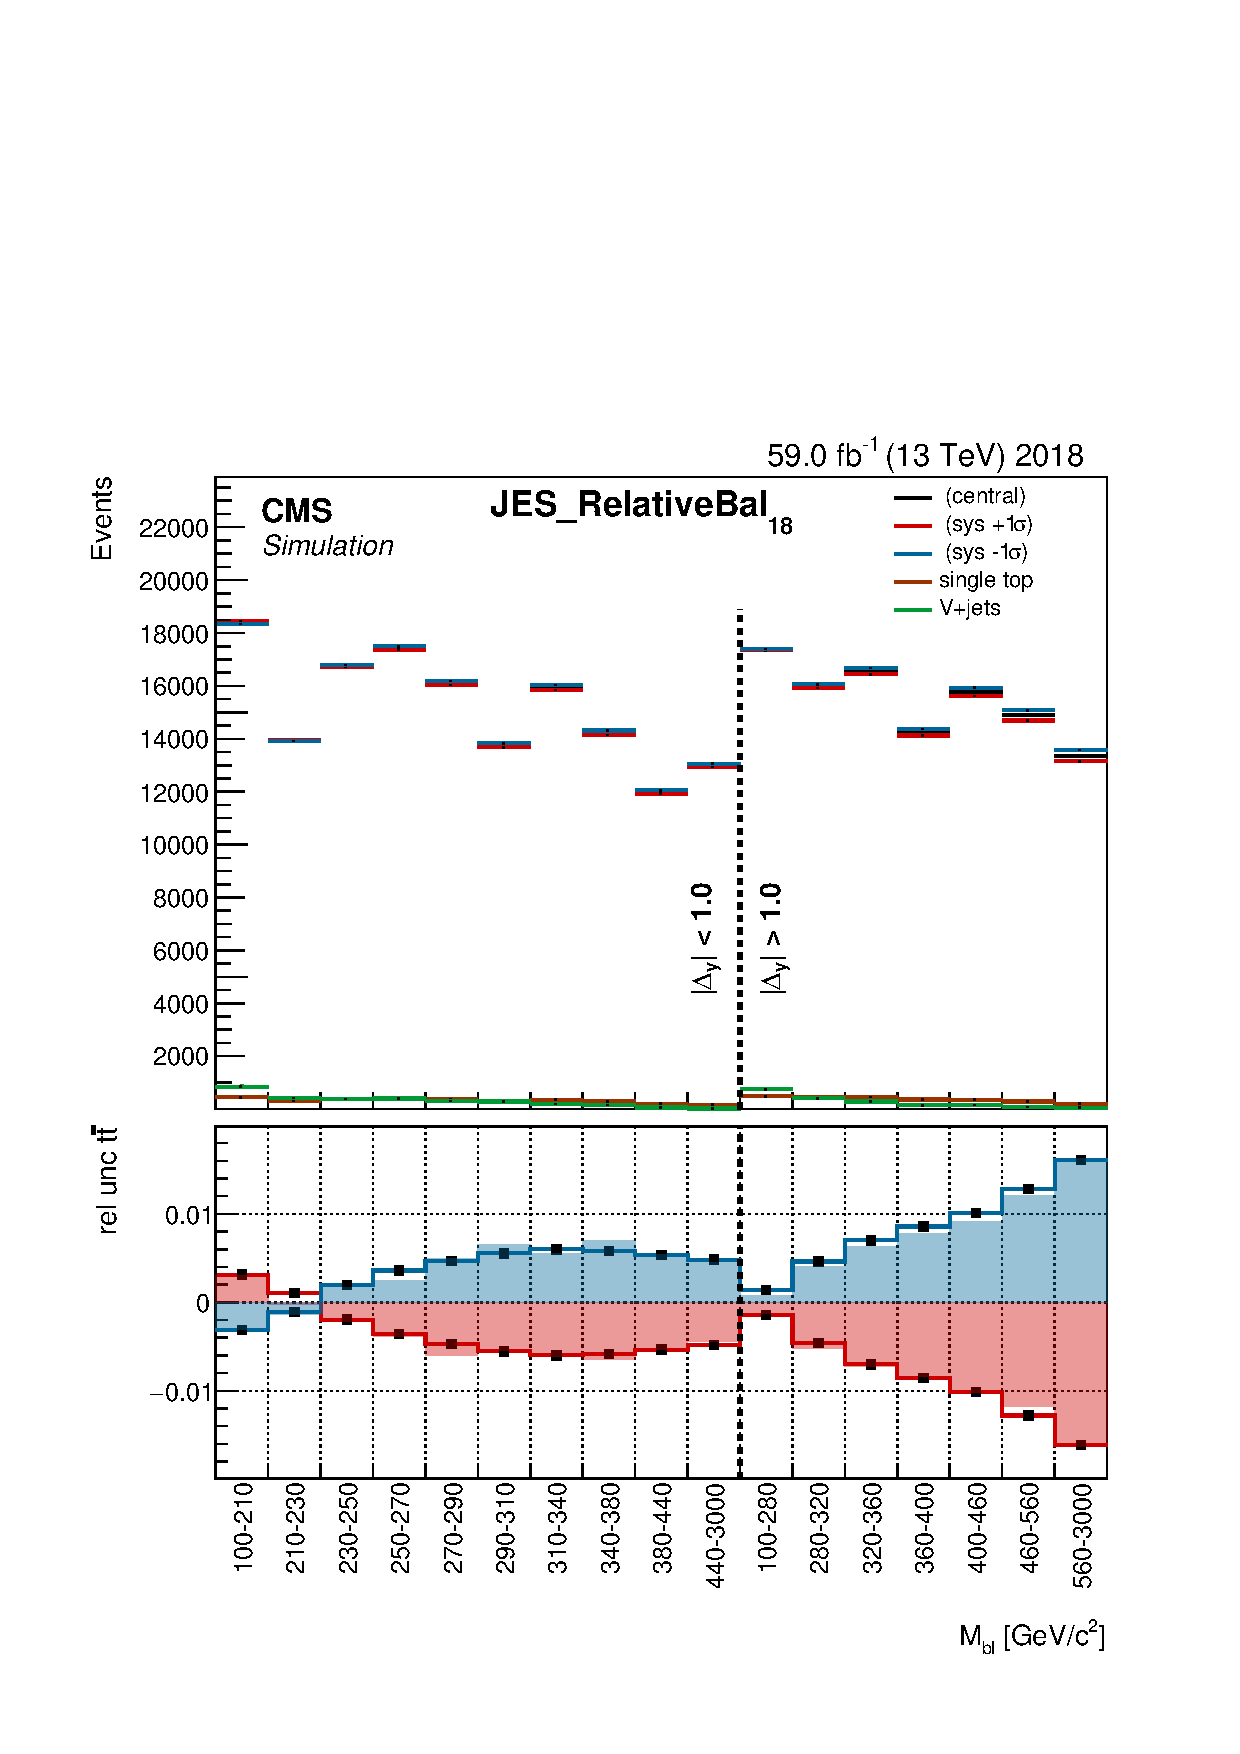
\includegraphics[width=.35\linewidth]{templates/JES_RelativeBal_18}
\caption{JES\_RelativeBal templates}
\label{fig:JES-RelativeBal_template}
\end{figure}

\begin{figure} \centering
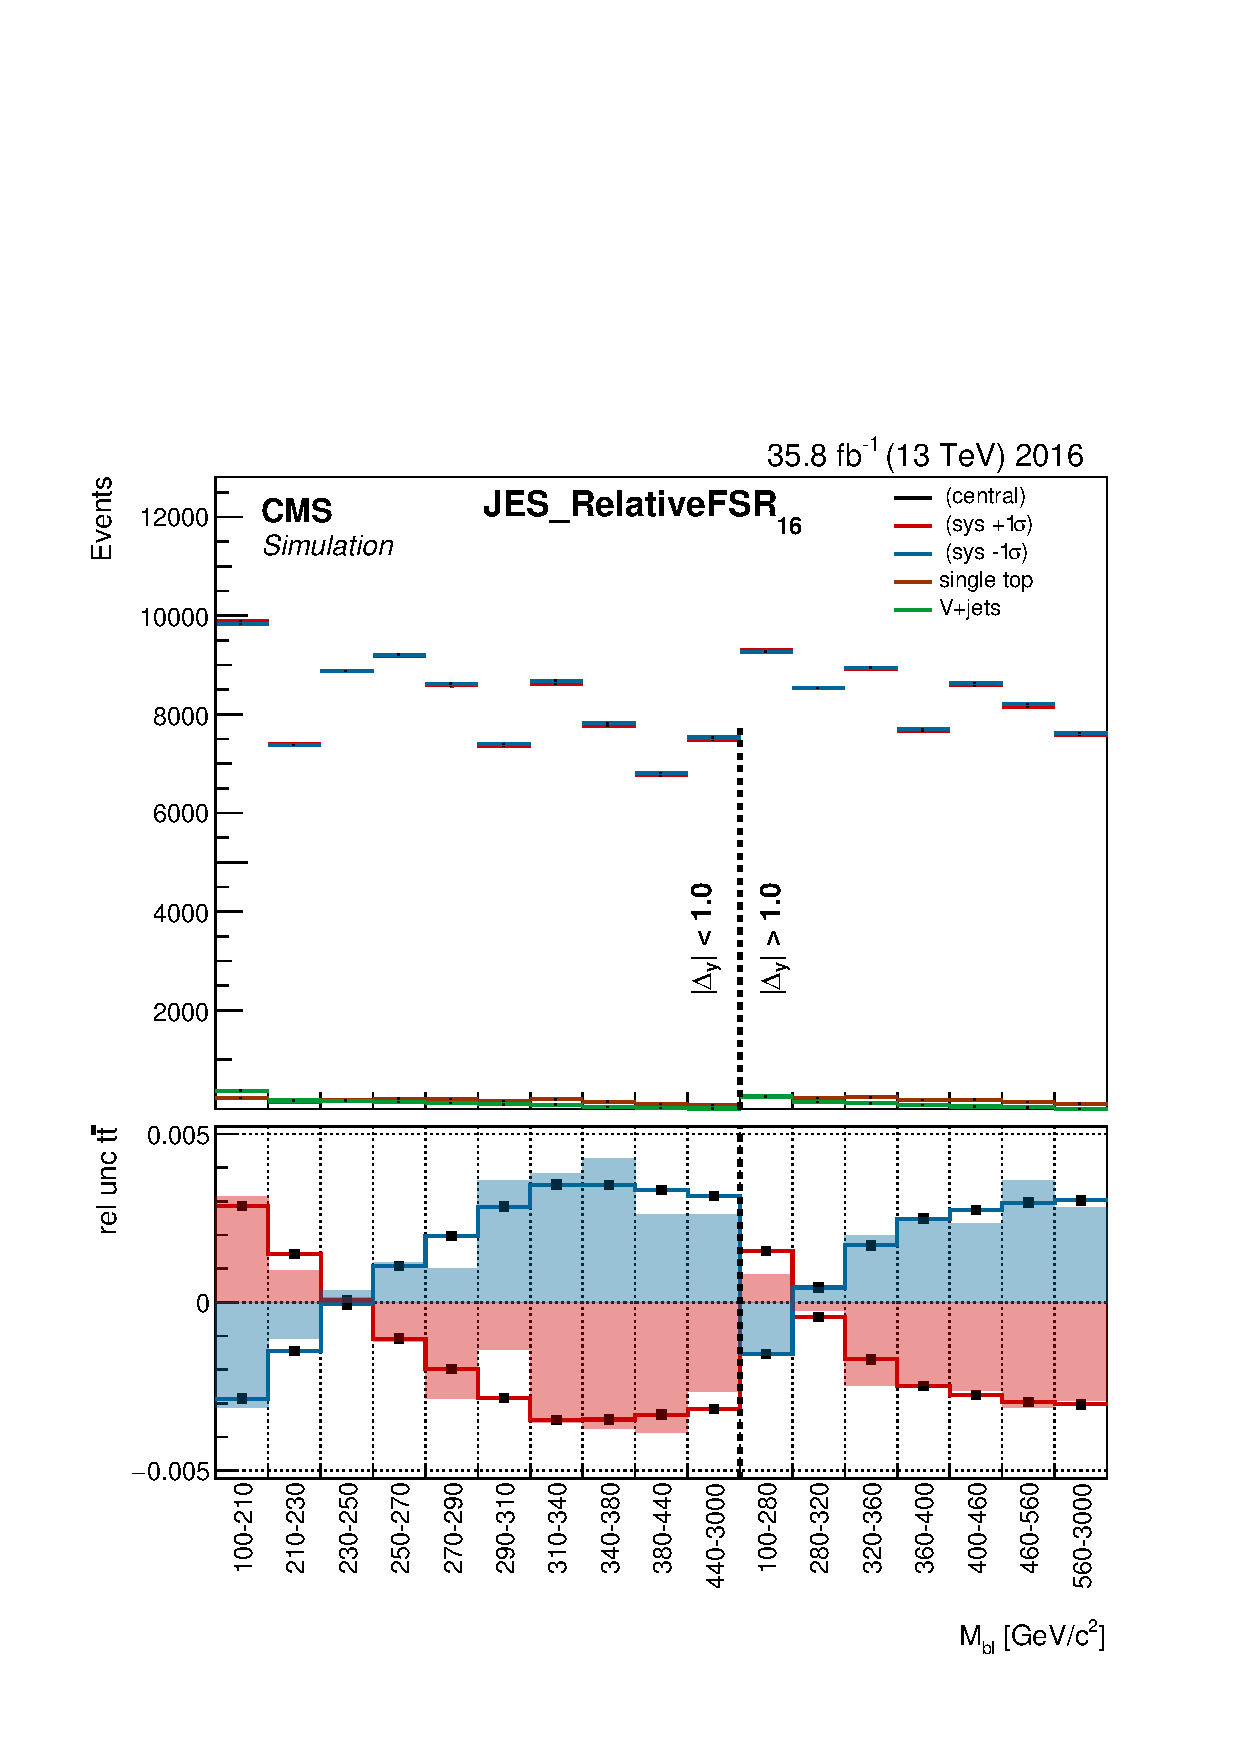
\includegraphics[width=.35\linewidth]{templates/JES_RelativeFSR_16}\hskip-.5cm
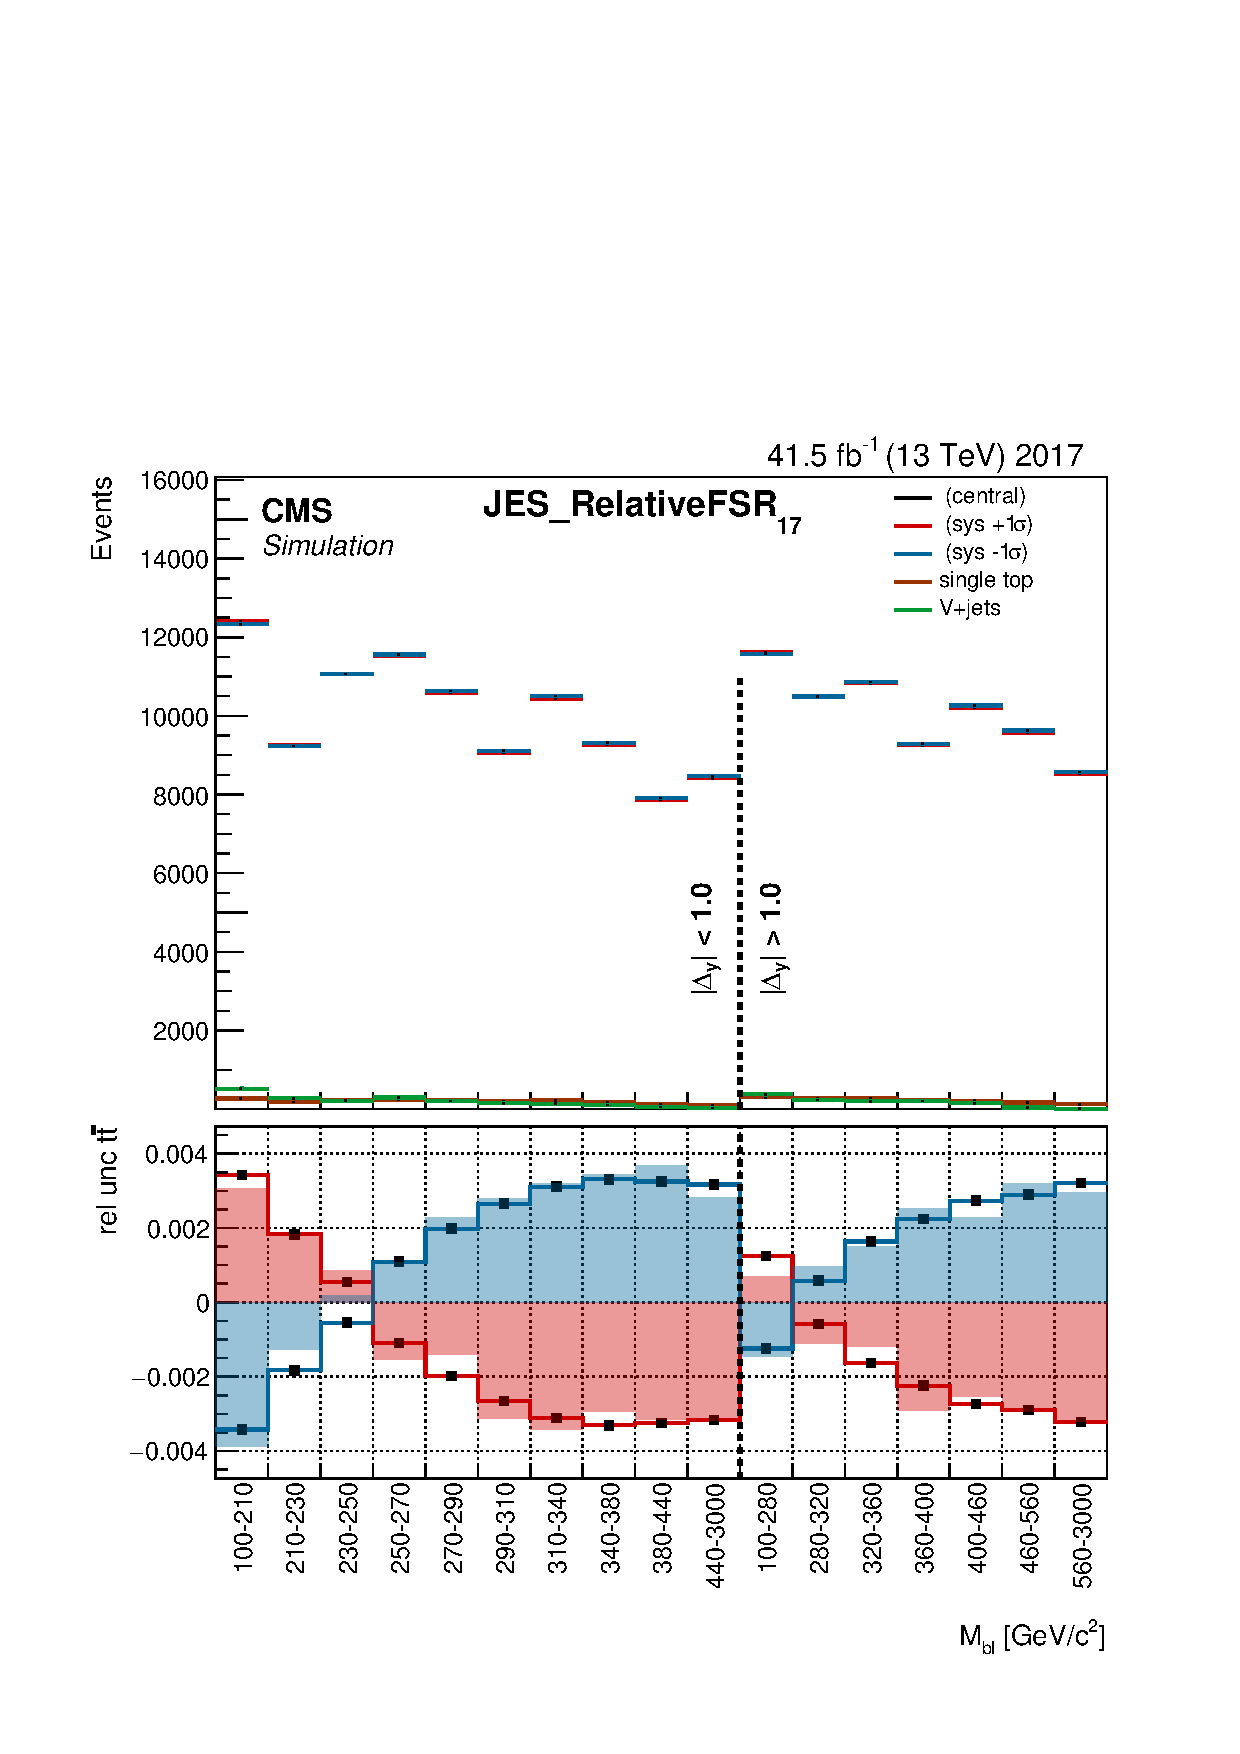
\includegraphics[width=.35\linewidth]{templates/JES_RelativeFSR_17}\hskip-.5cm
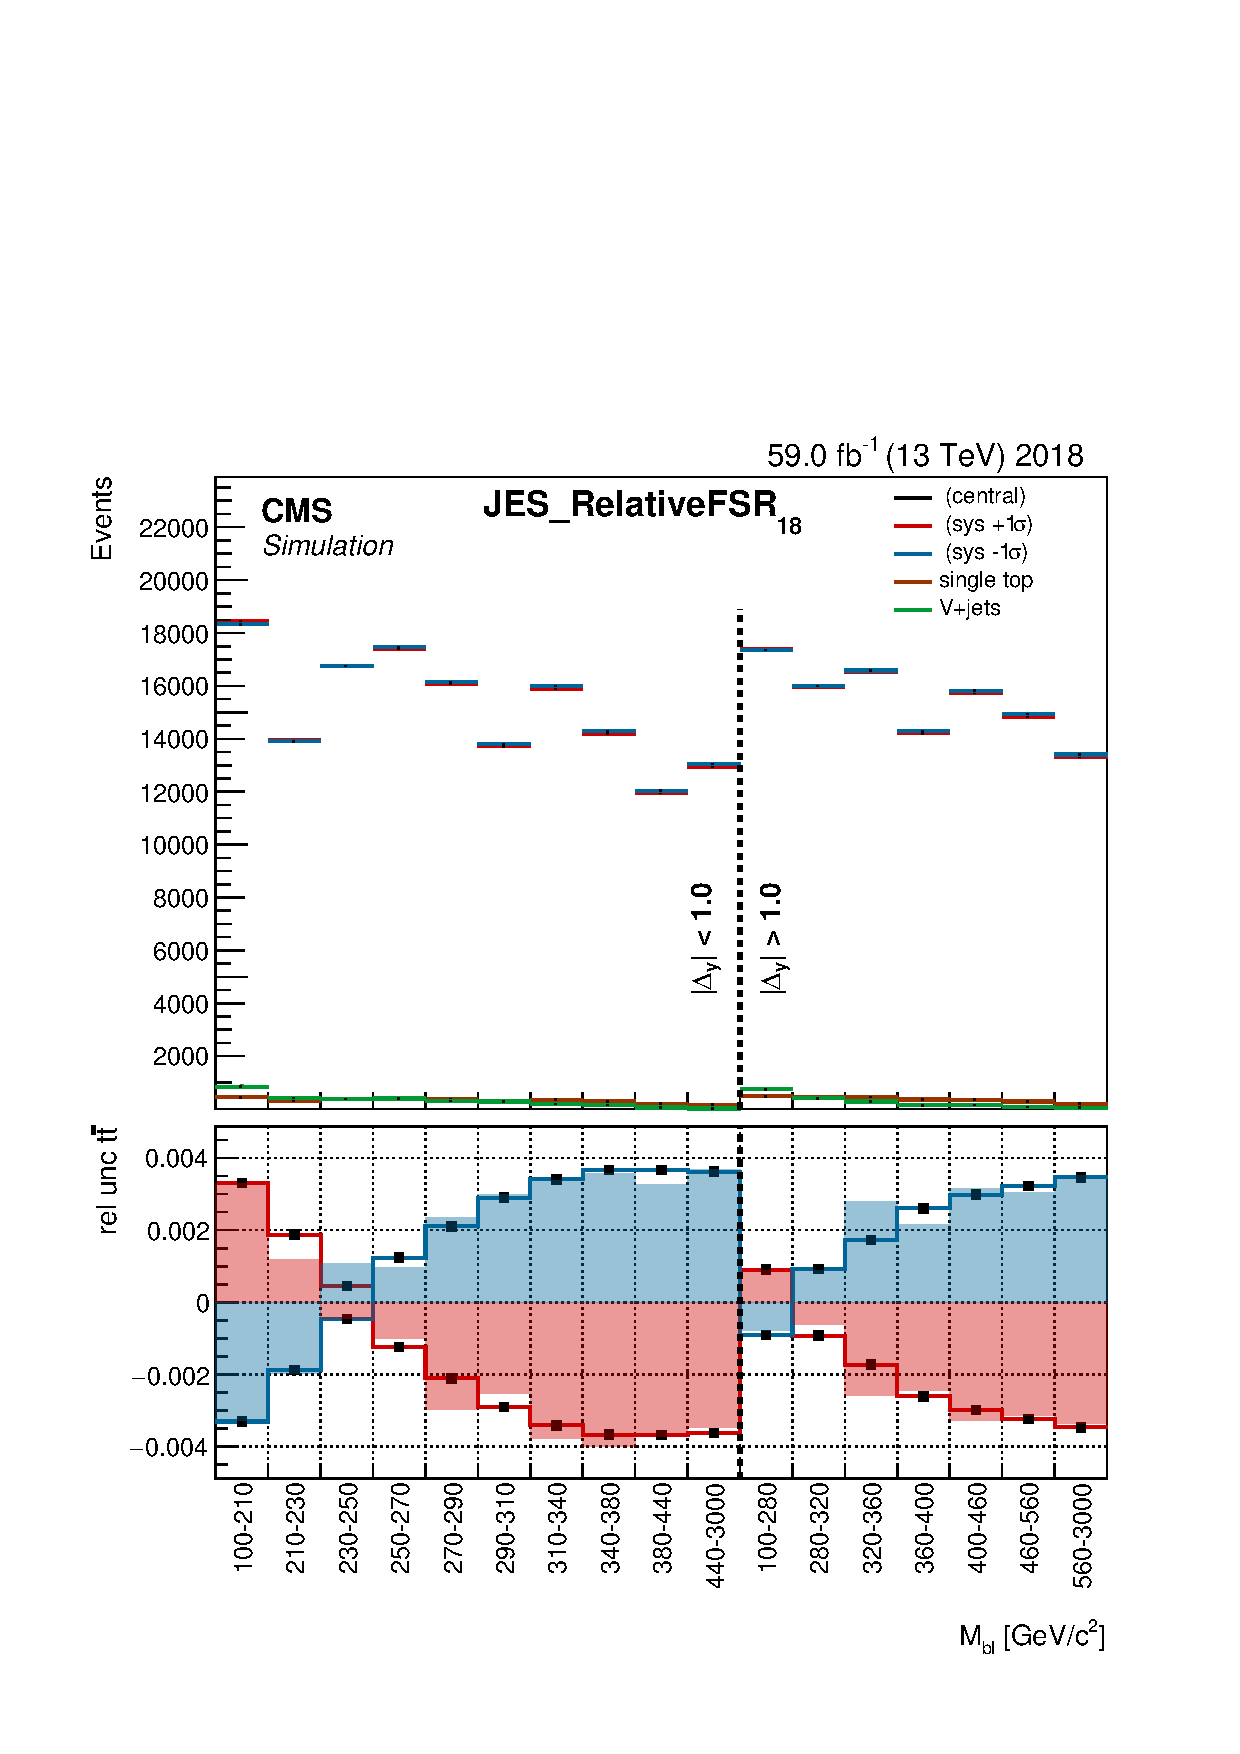
\includegraphics[width=.35\linewidth]{templates/JES_RelativeFSR_18}
\caption{JES\_RelativeFSR templates}
\label{fig:JES-RelativeFSR_template}
\end{figure}

\begin{figure} \centering
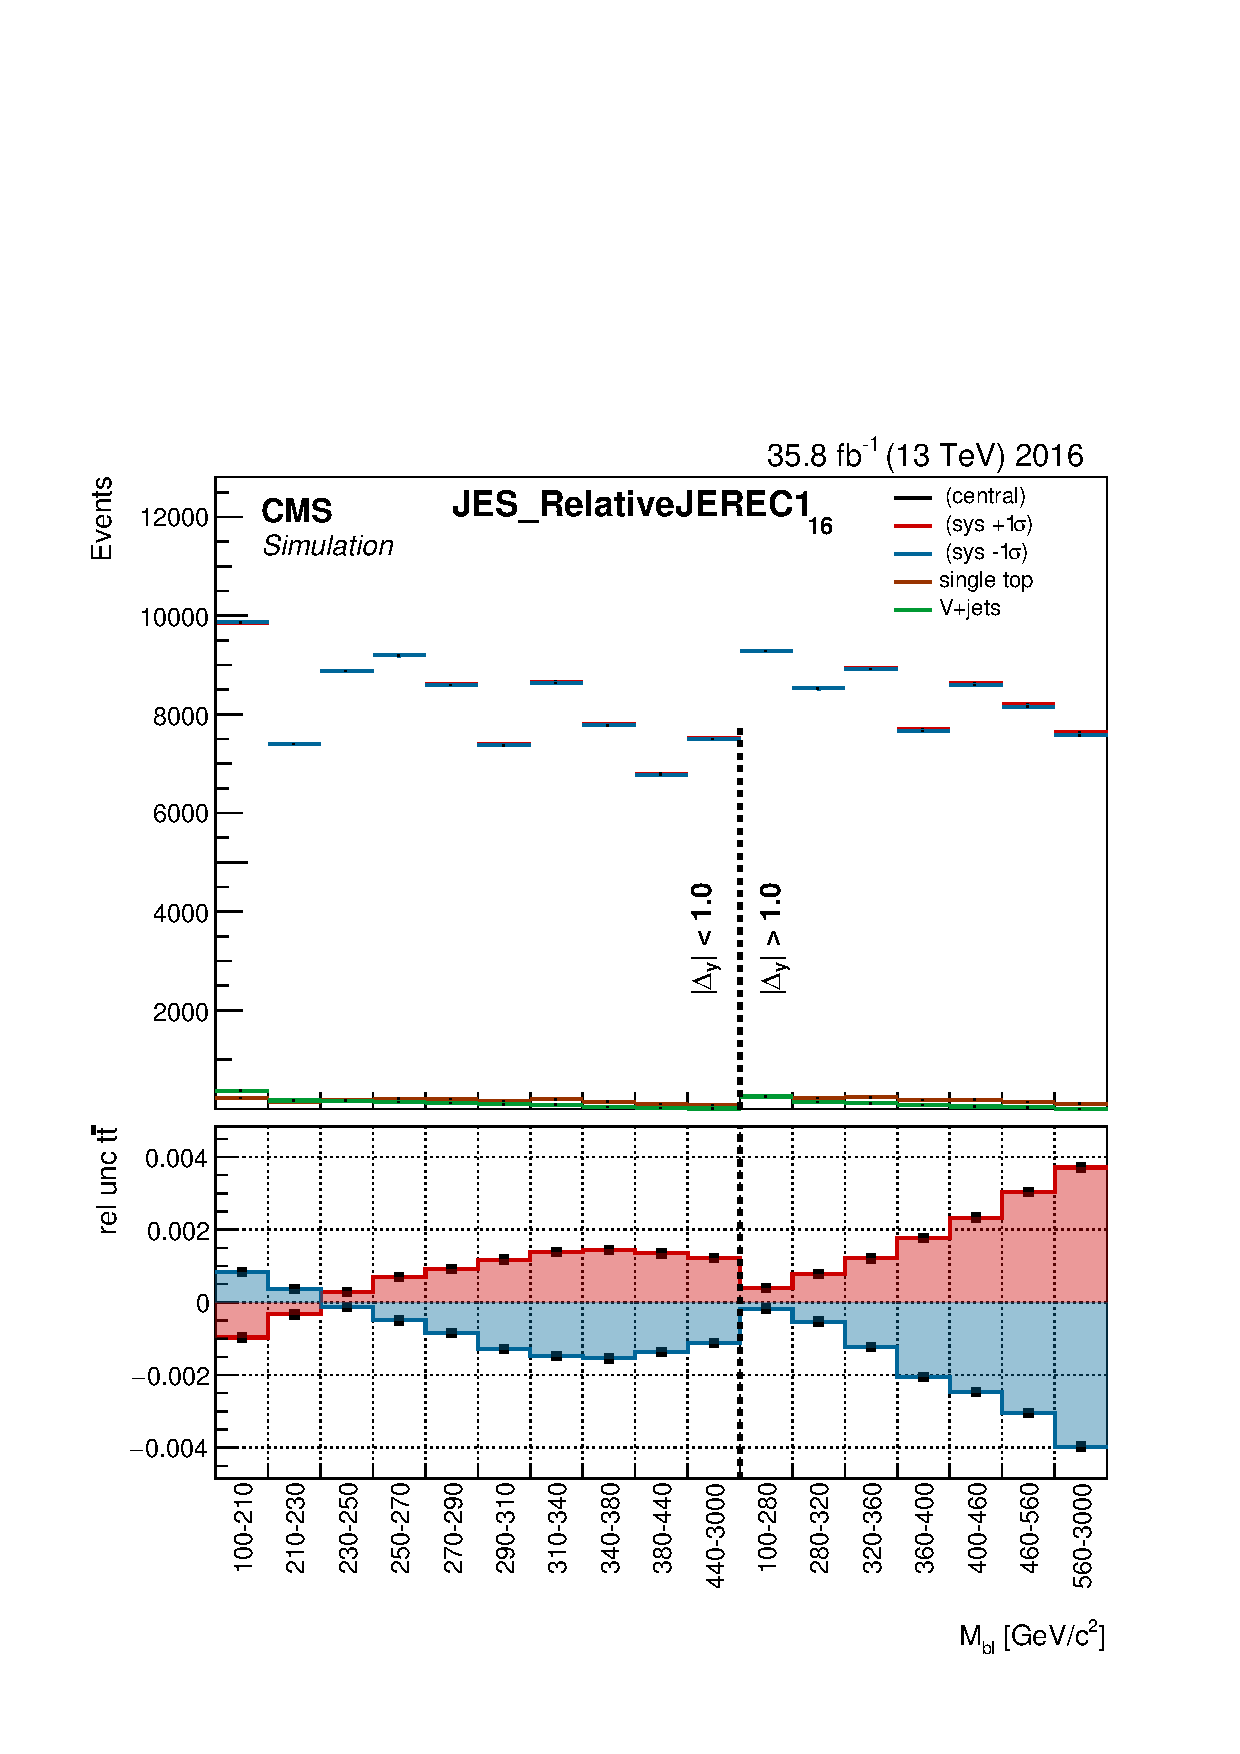
\includegraphics[width=.35\linewidth]{templates/JES_RelativeJEREC1_16}\hskip-.5cm
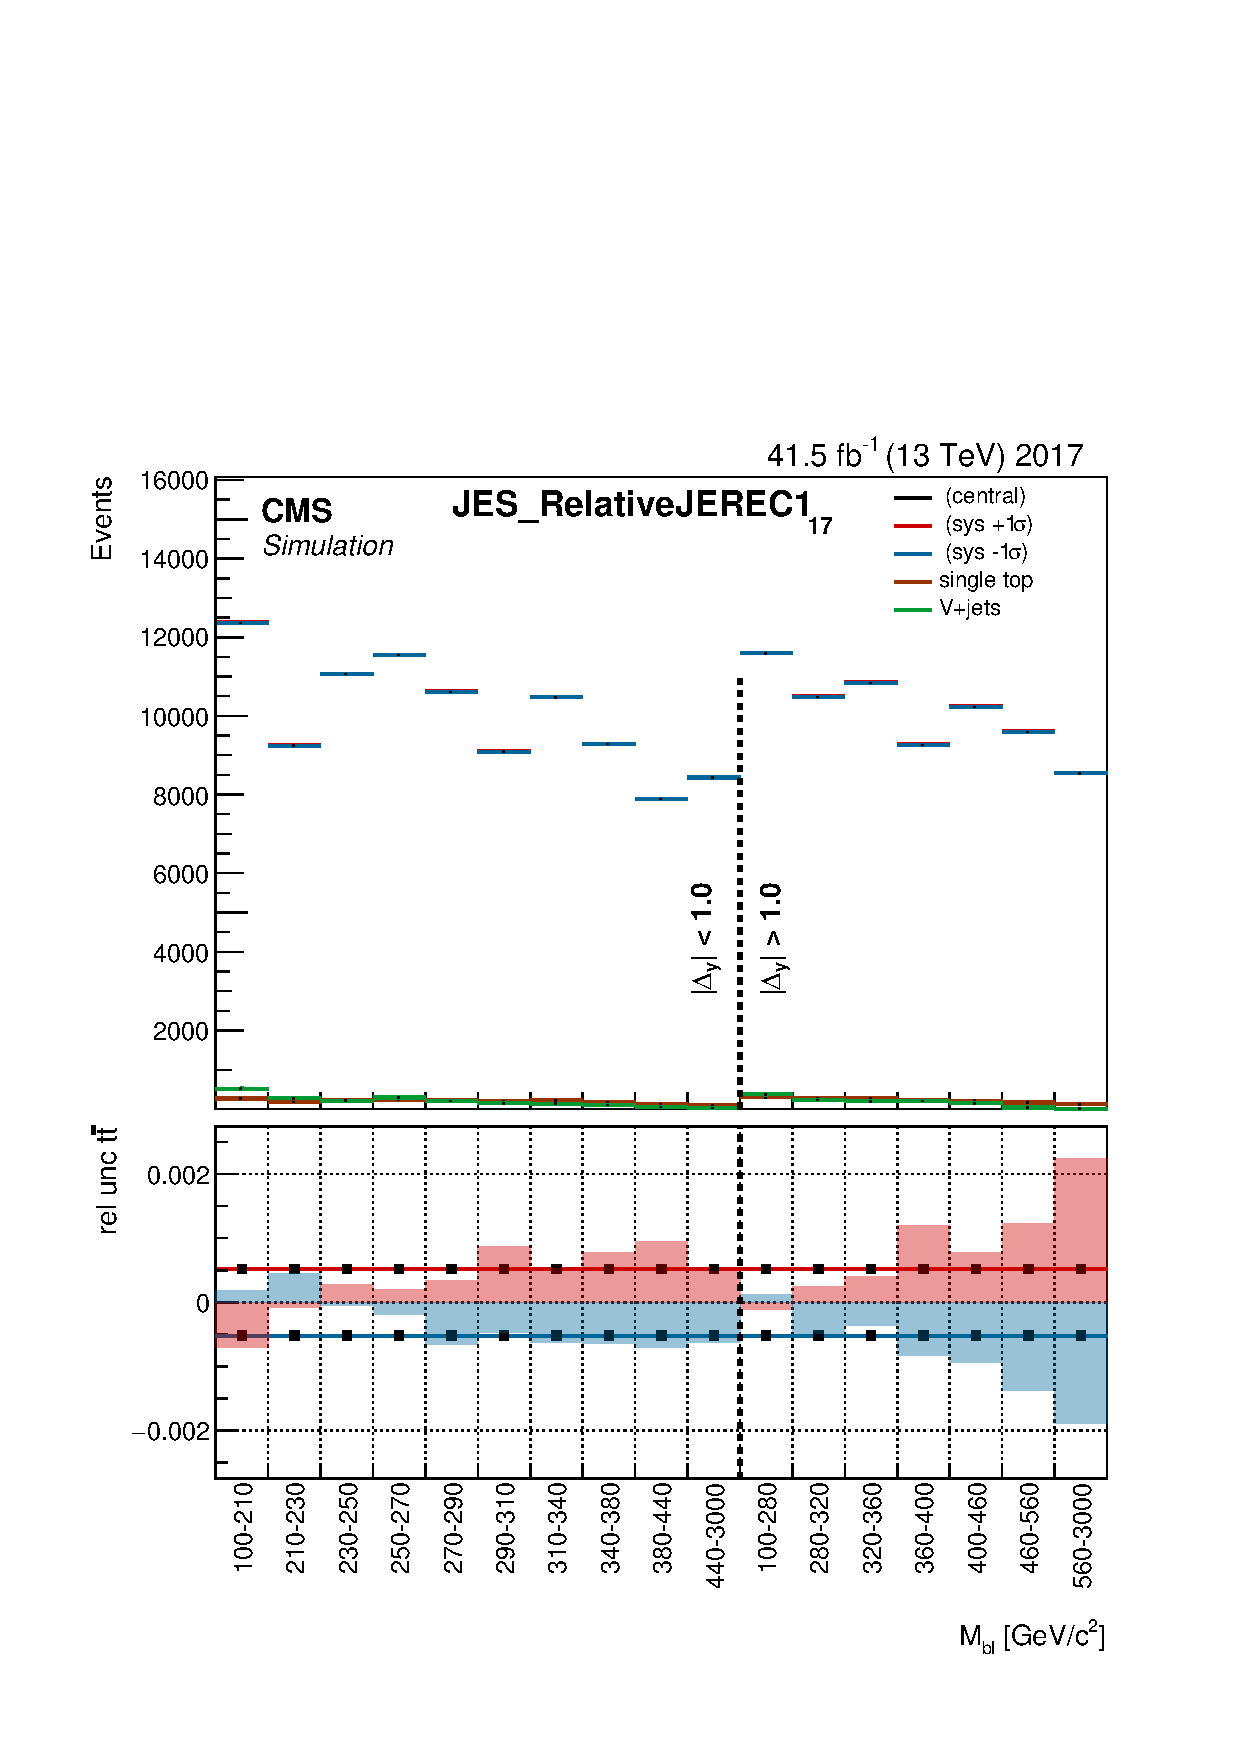
\includegraphics[width=.35\linewidth]{templates/JES_RelativeJEREC1_17}\hskip-.5cm
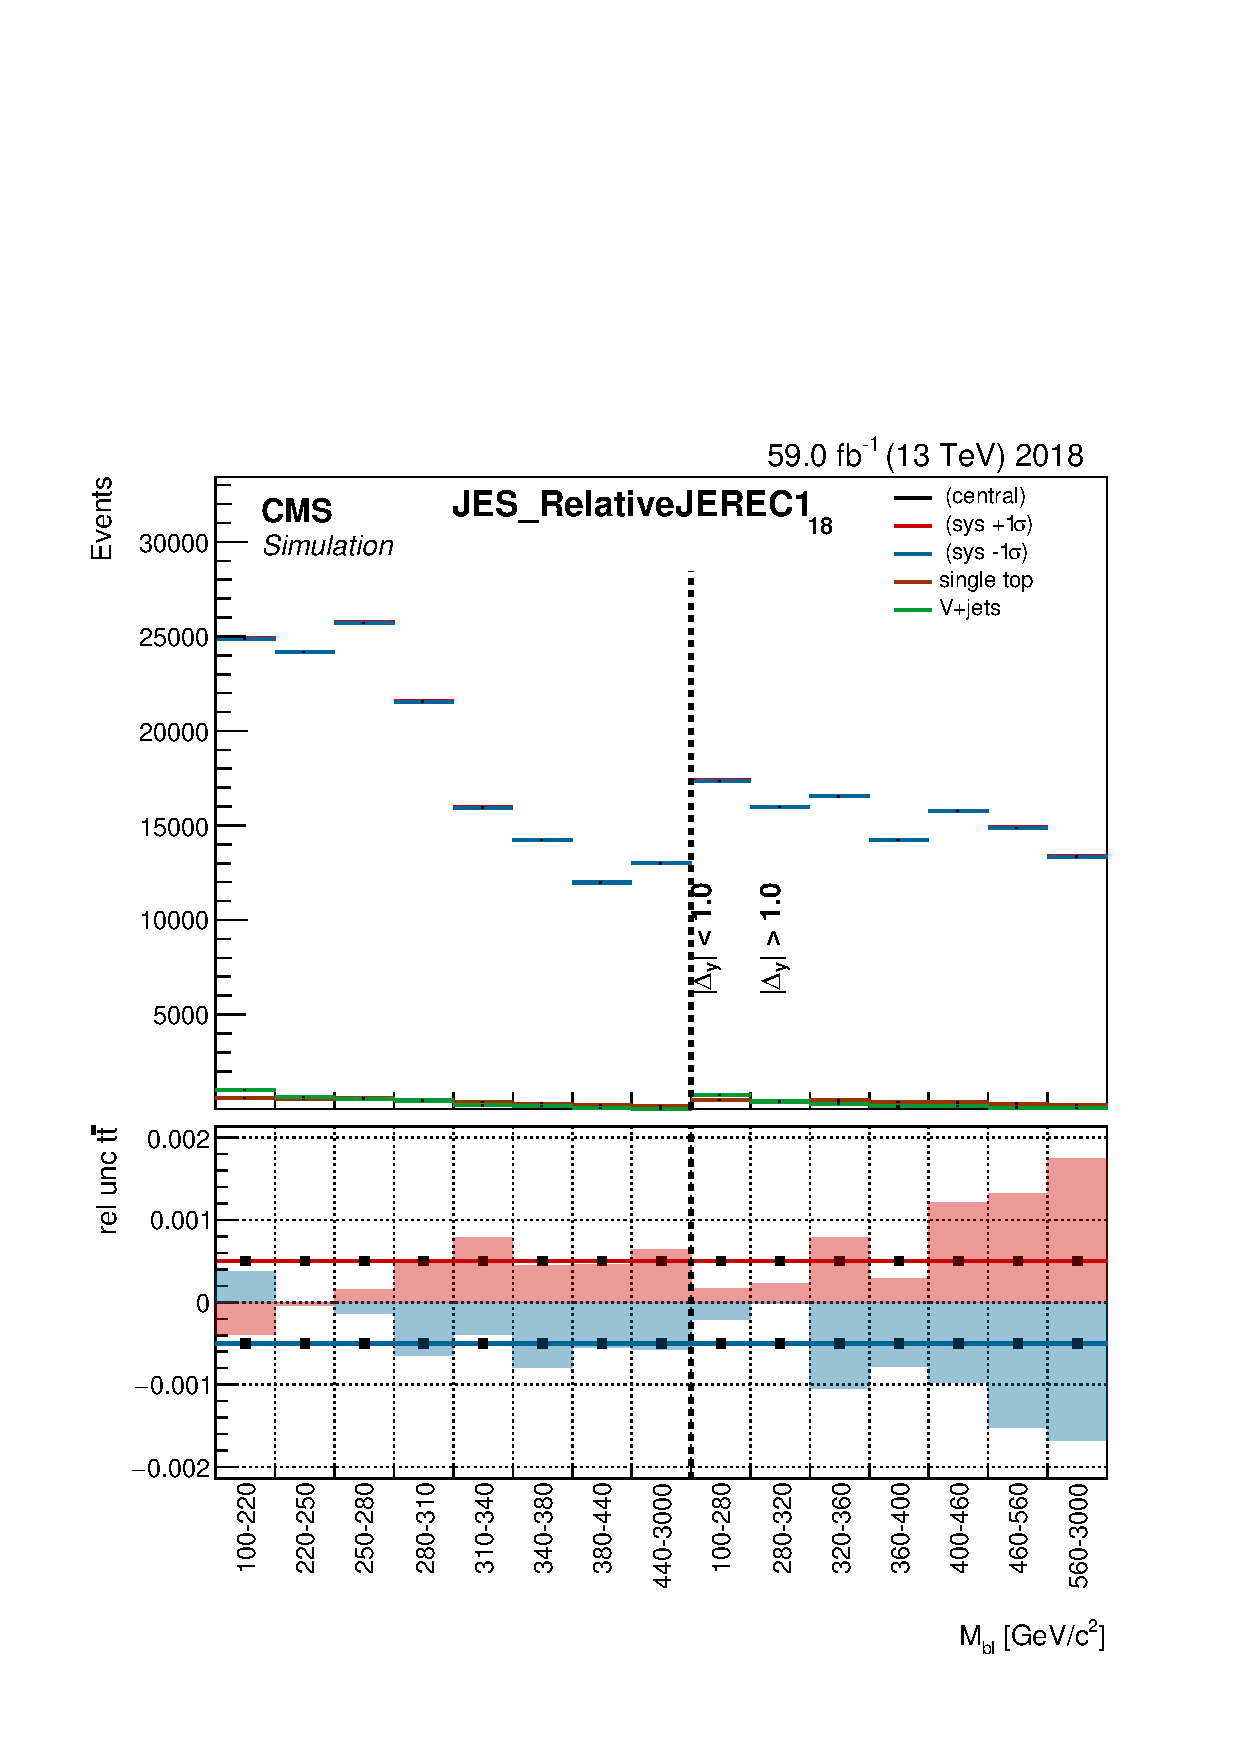
\includegraphics[width=.35\linewidth]{templates/JES_RelativeJEREC1_18}
\caption{JES\_RelativeJEREC1 templates}
\label{fig:JES-RelativeJEREC1_template}
\end{figure}

\begin{figure} \centering
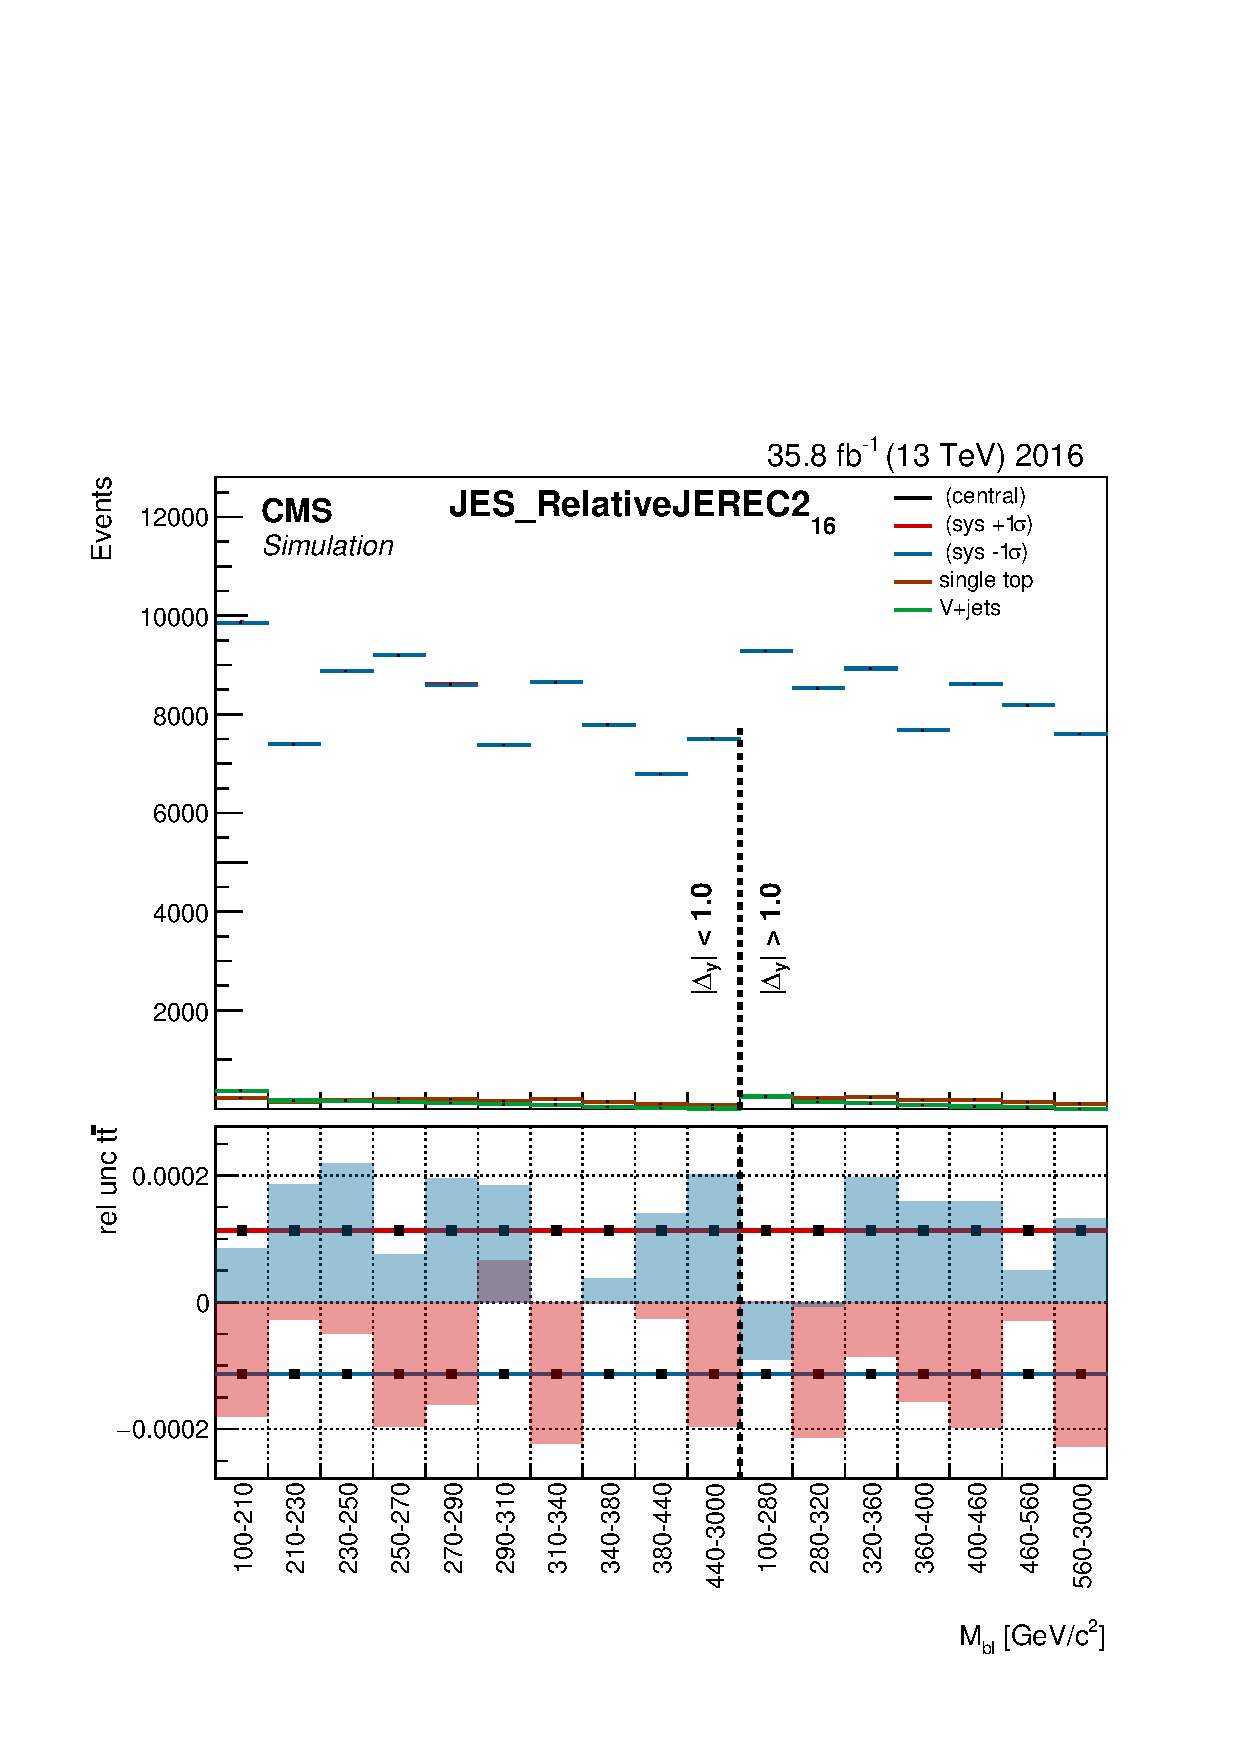
\includegraphics[width=.35\linewidth]{templates/JES_RelativeJEREC2_16}\hskip-.5cm
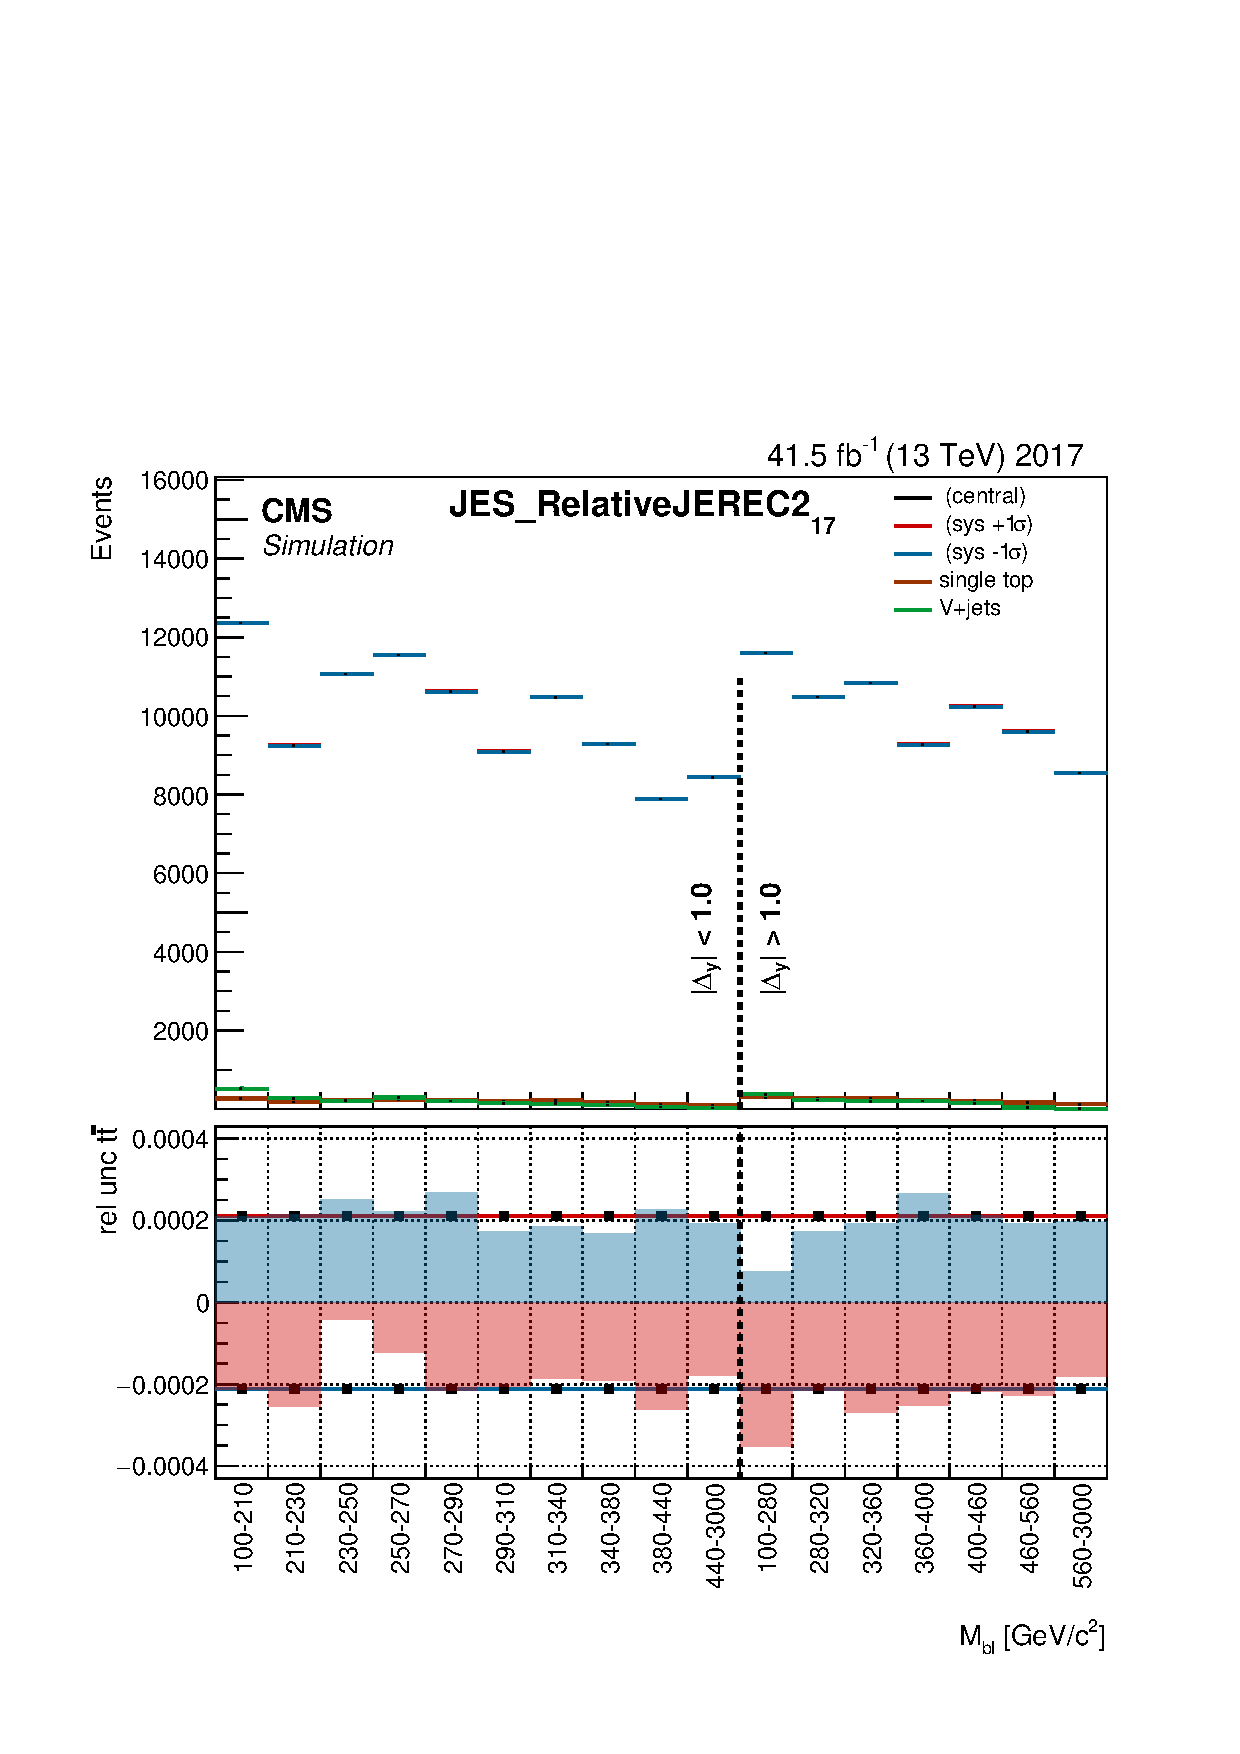
\includegraphics[width=.35\linewidth]{templates/JES_RelativeJEREC2_17}\hskip-.5cm
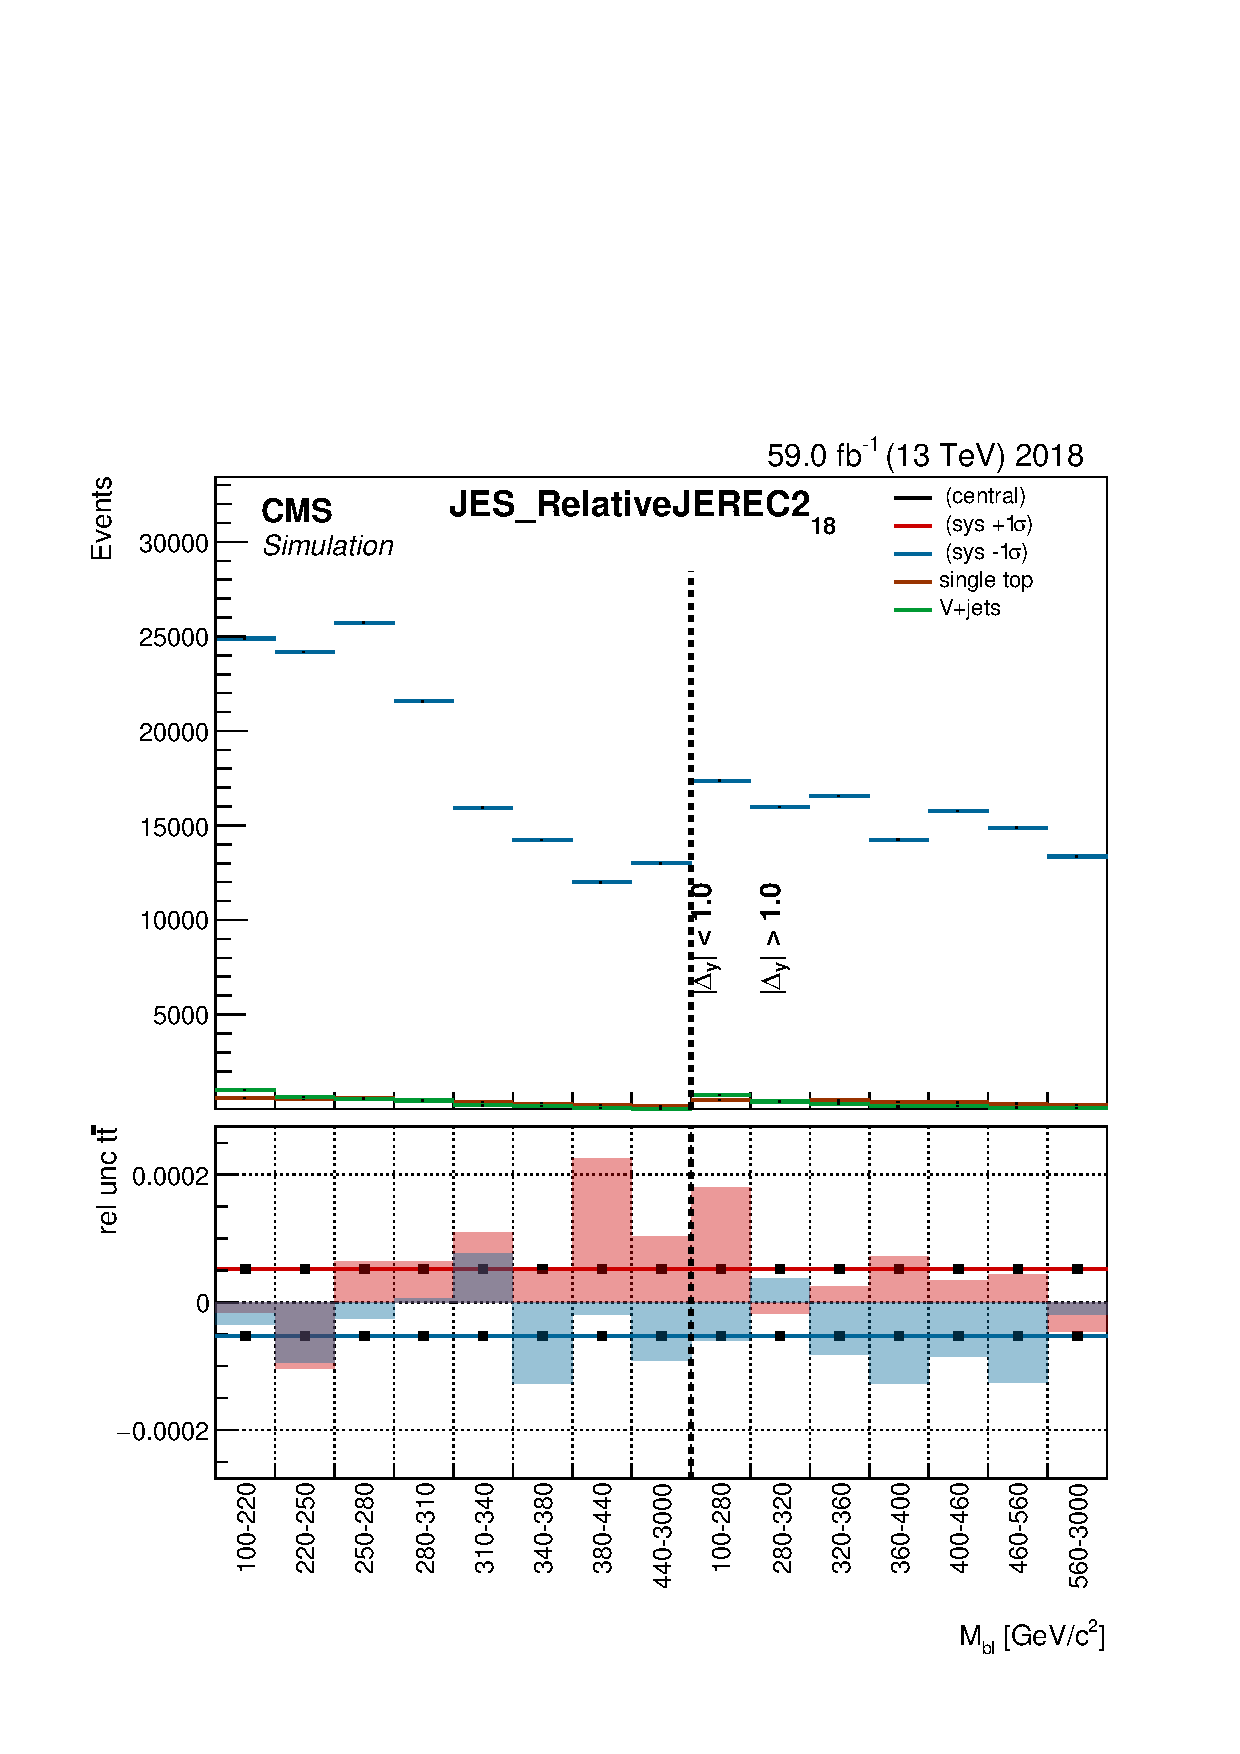
\includegraphics[width=.35\linewidth]{templates/JES_RelativeJEREC2_18}
\caption{JES\_RelativeJEREC2 templates}
\label{fig:JES-RelativeJEREC2_template}
\end{figure}

\begin{figure} \centering
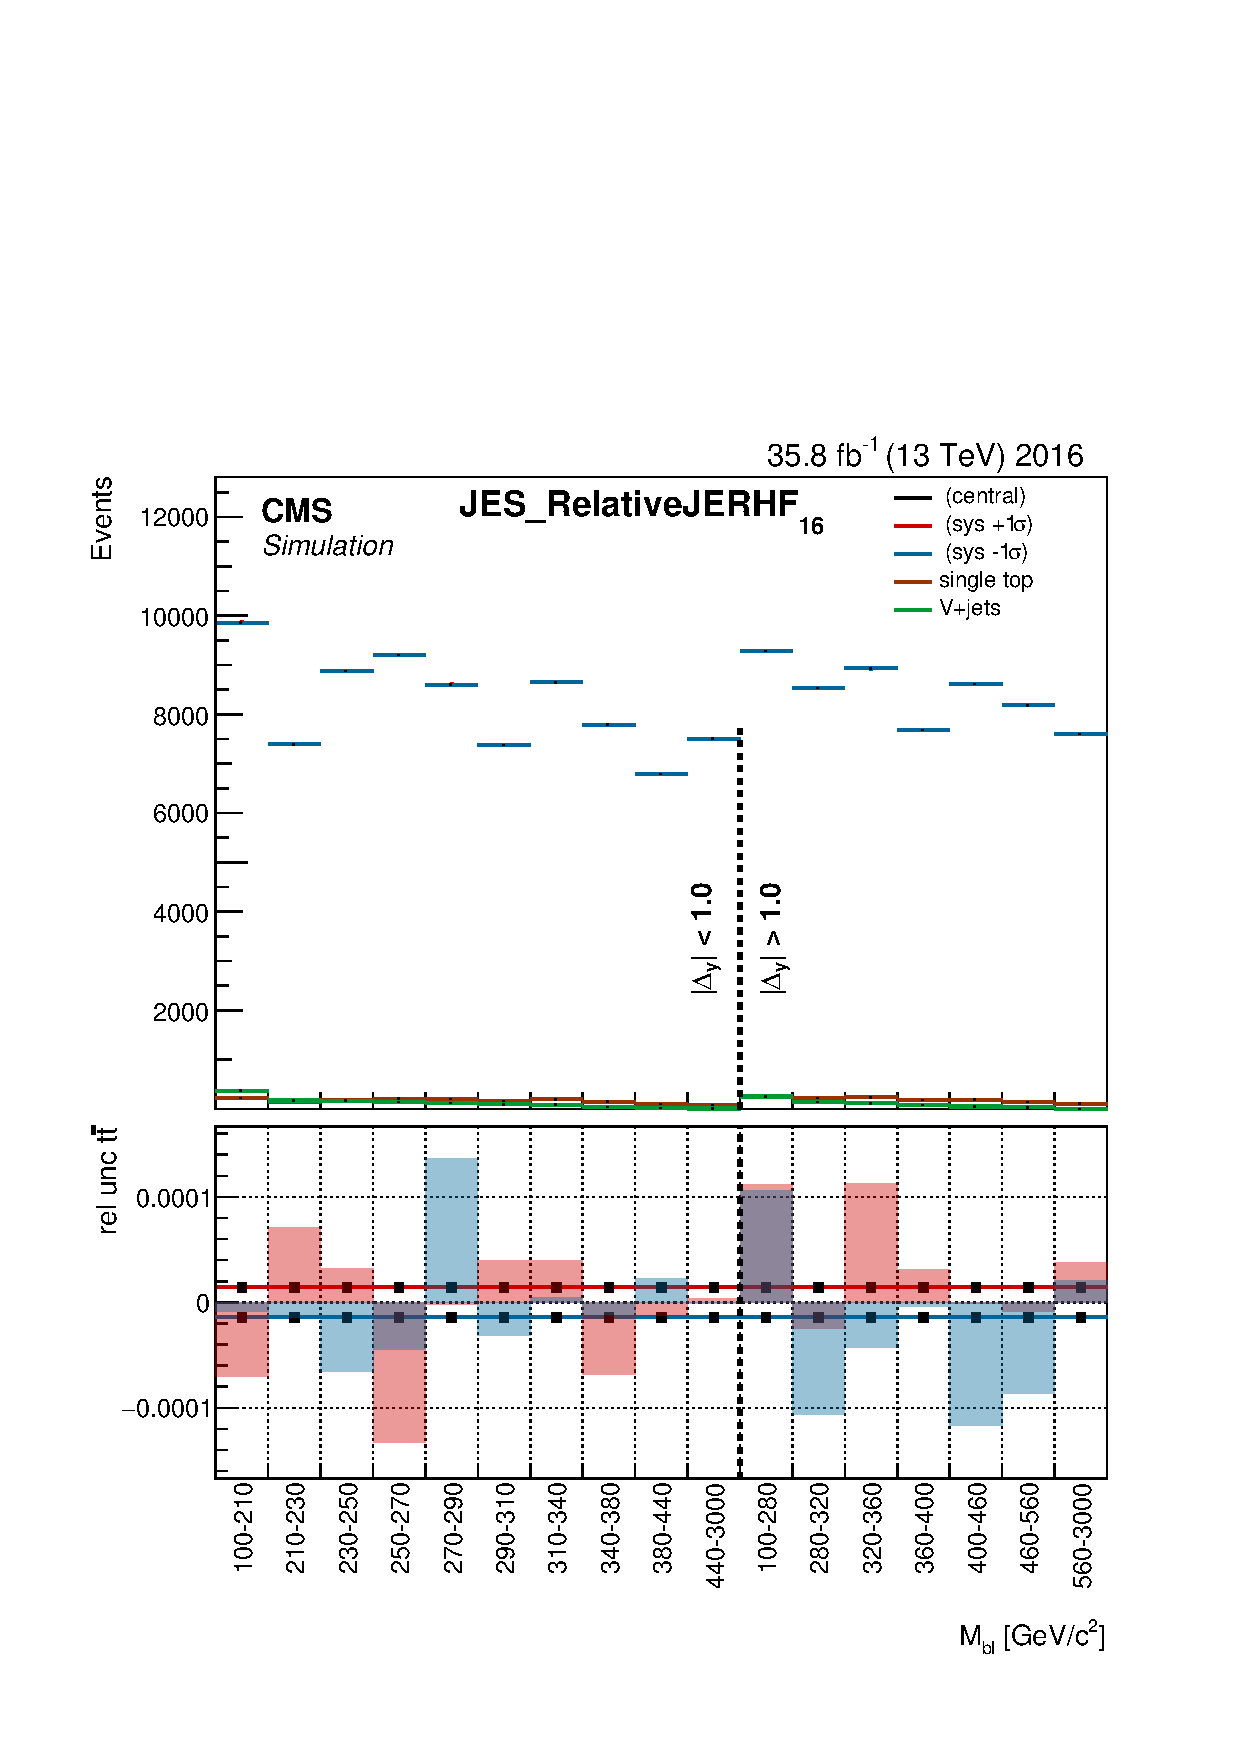
\includegraphics[width=.35\linewidth]{templates/JES_RelativeJERHF_16}\hskip-.5cm
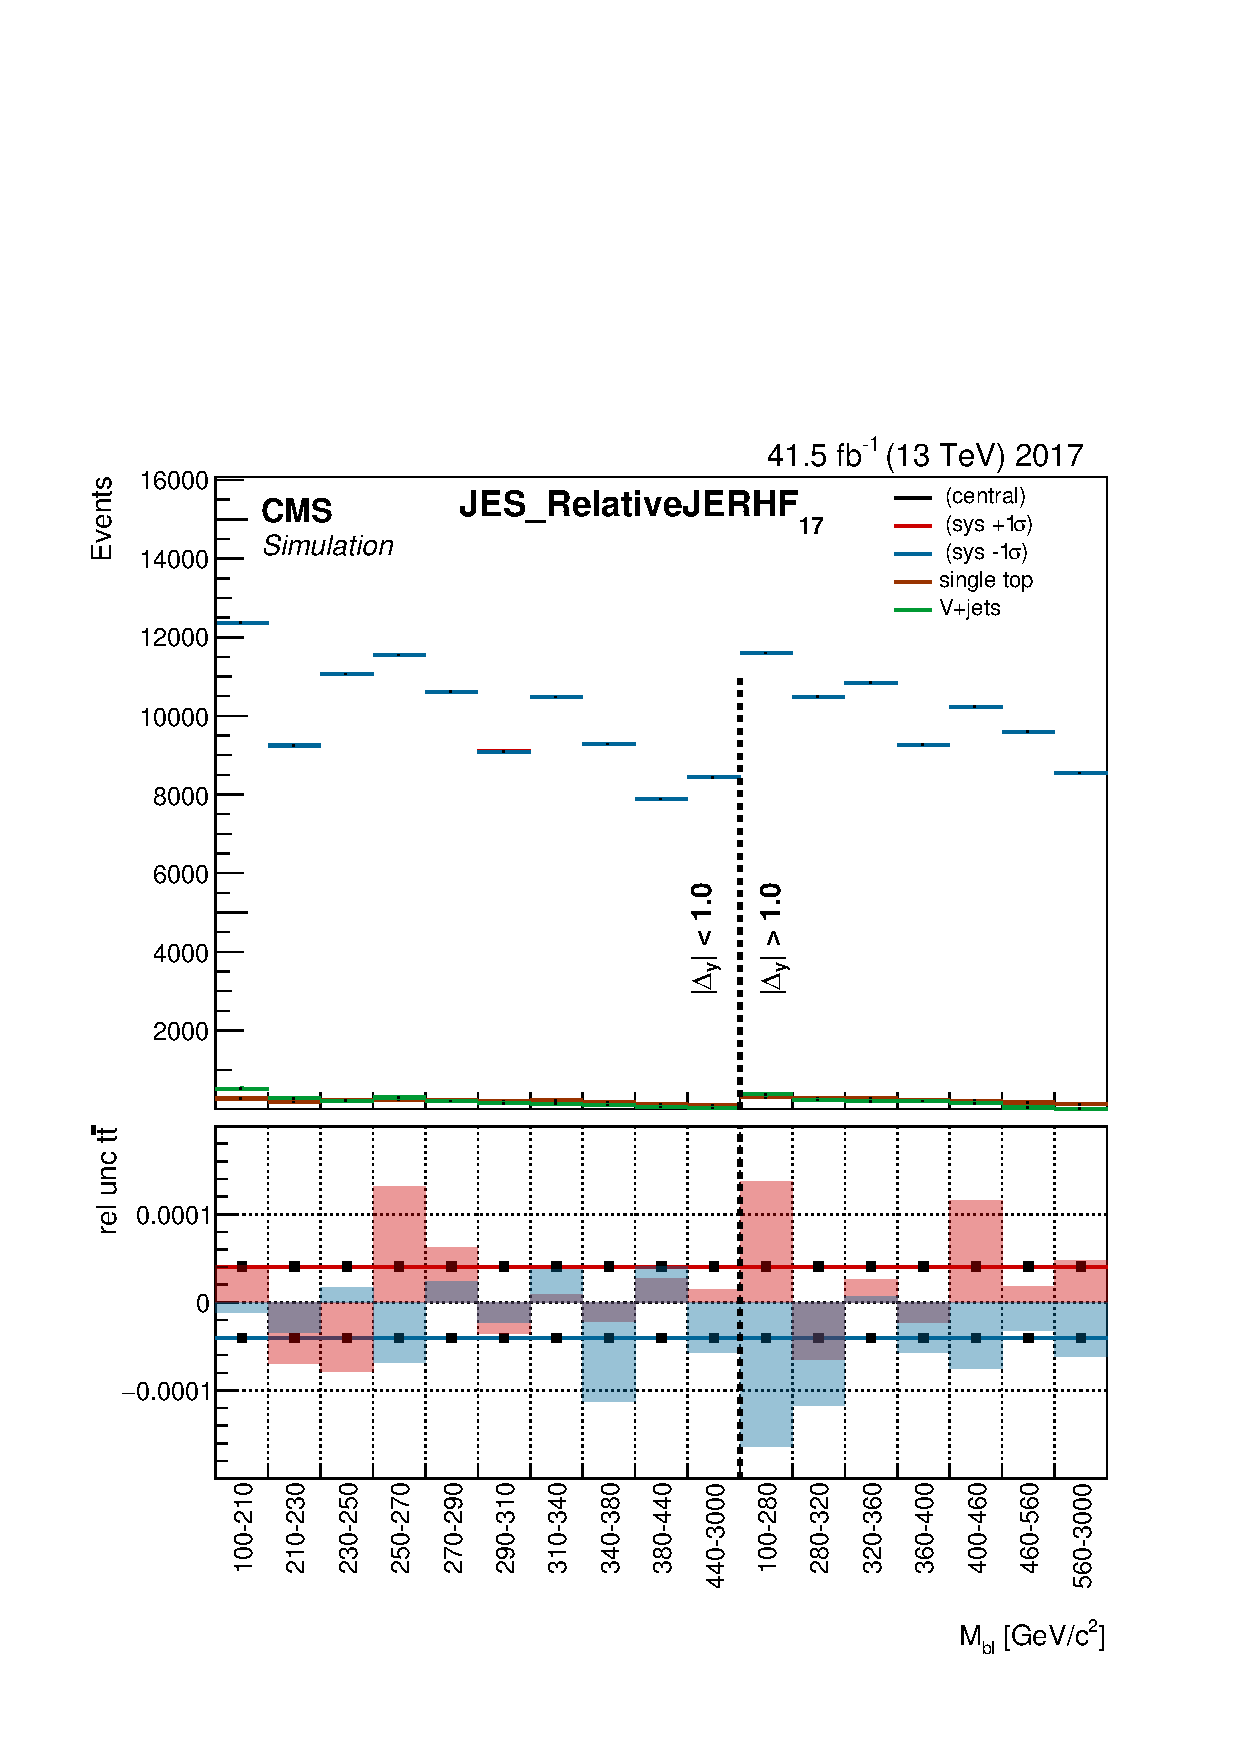
\includegraphics[width=.35\linewidth]{templates/JES_RelativeJERHF_17}\hskip-.5cm
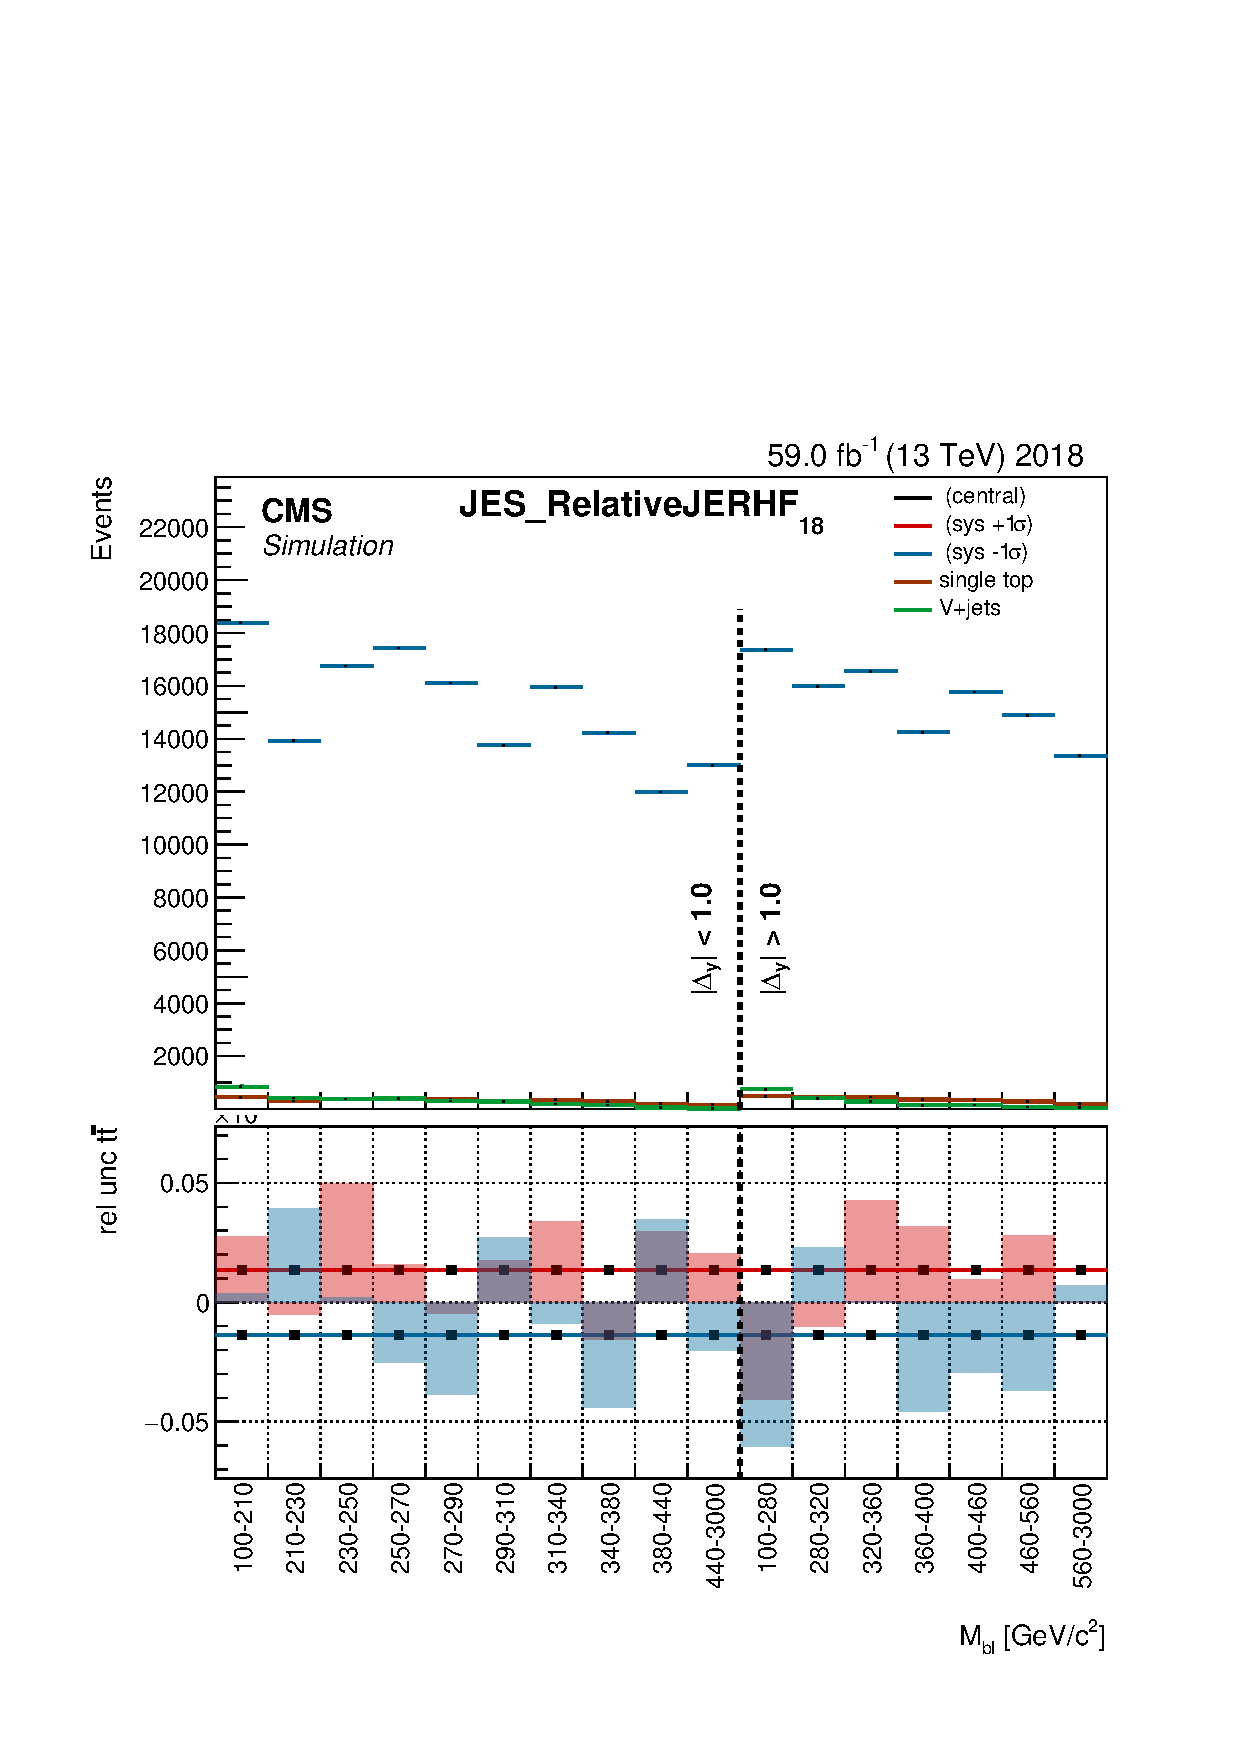
\includegraphics[width=.35\linewidth]{templates/JES_RelativeJERHF_18}
\caption{JES\_RelativeJERHF templates}
\label{fig:JES-RelativeJERHF_template}
\end{figure}

\begin{figure} \centering
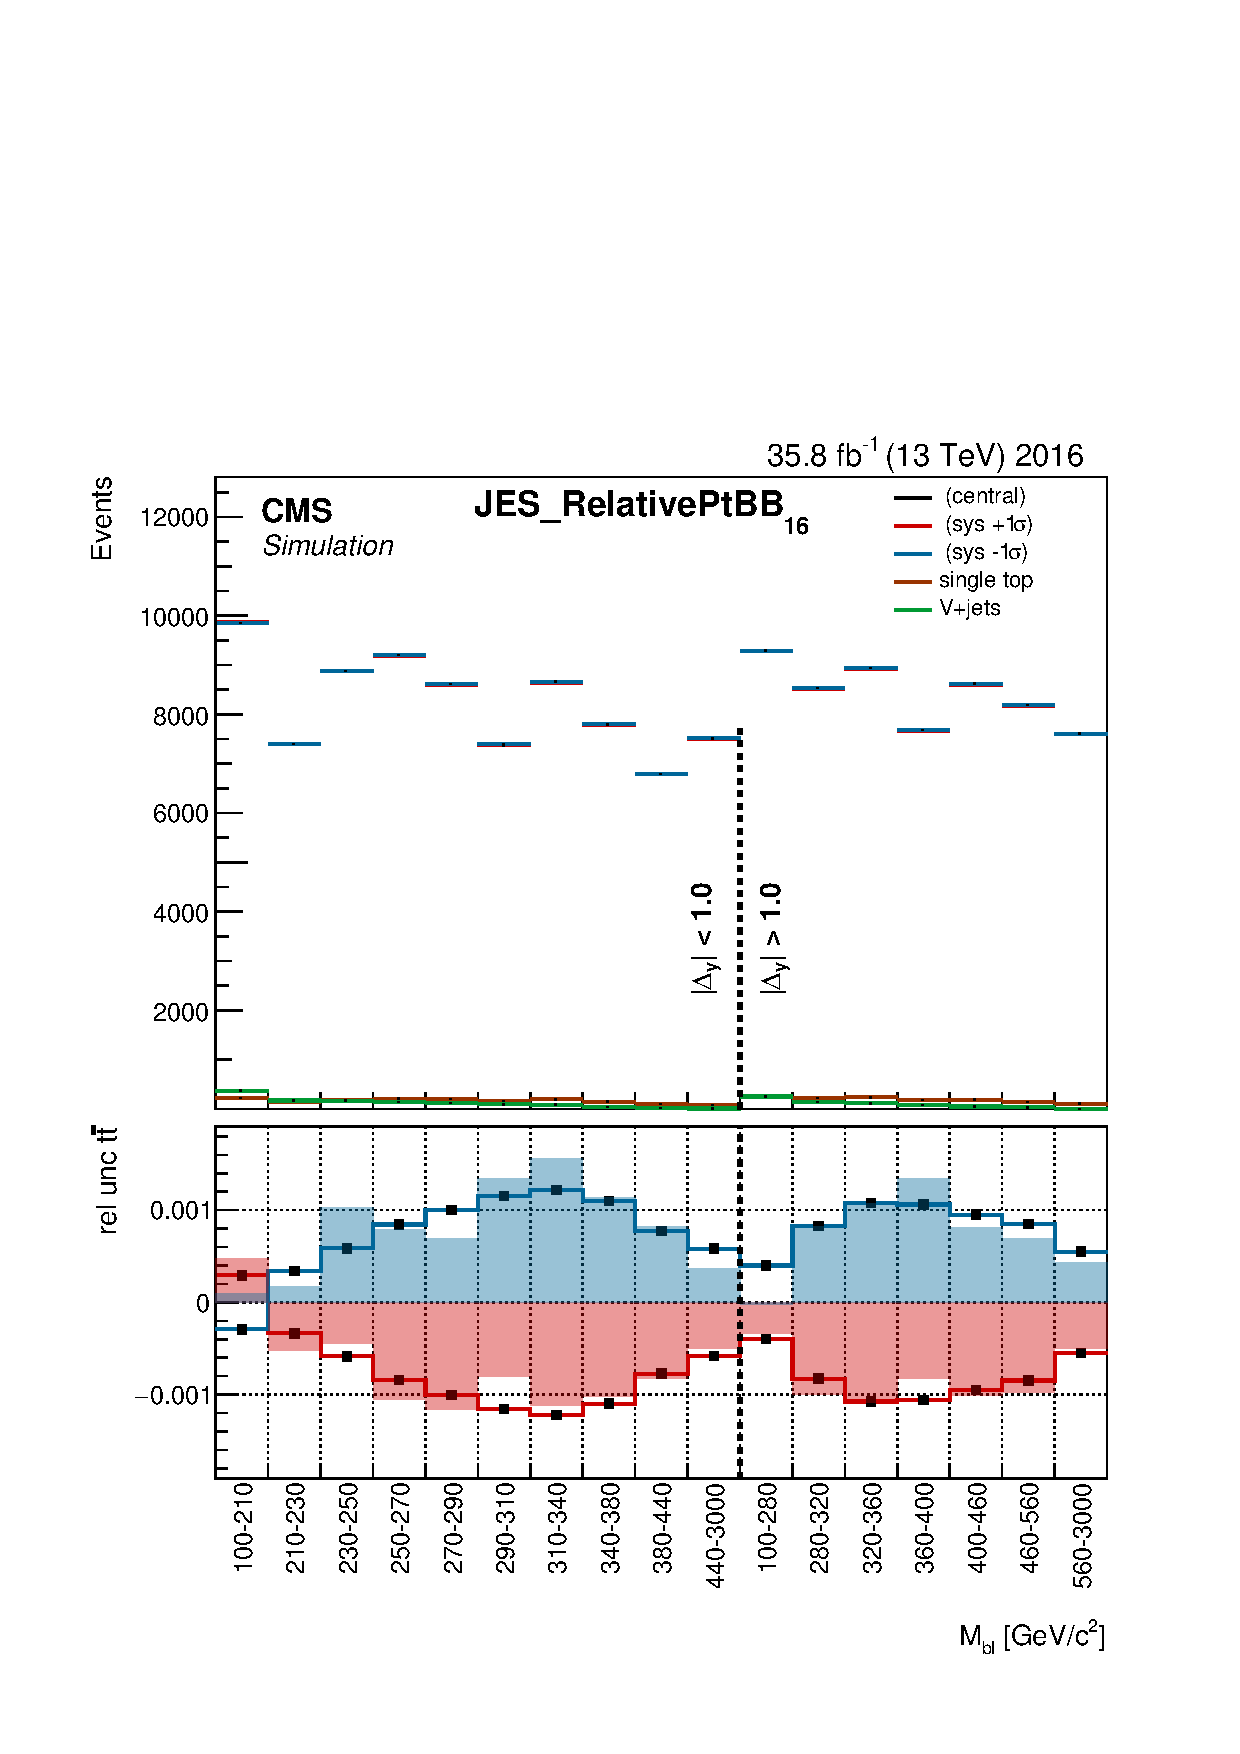
\includegraphics[width=.35\linewidth]{templates/JES_RelativePtBB_16}\hskip-.5cm
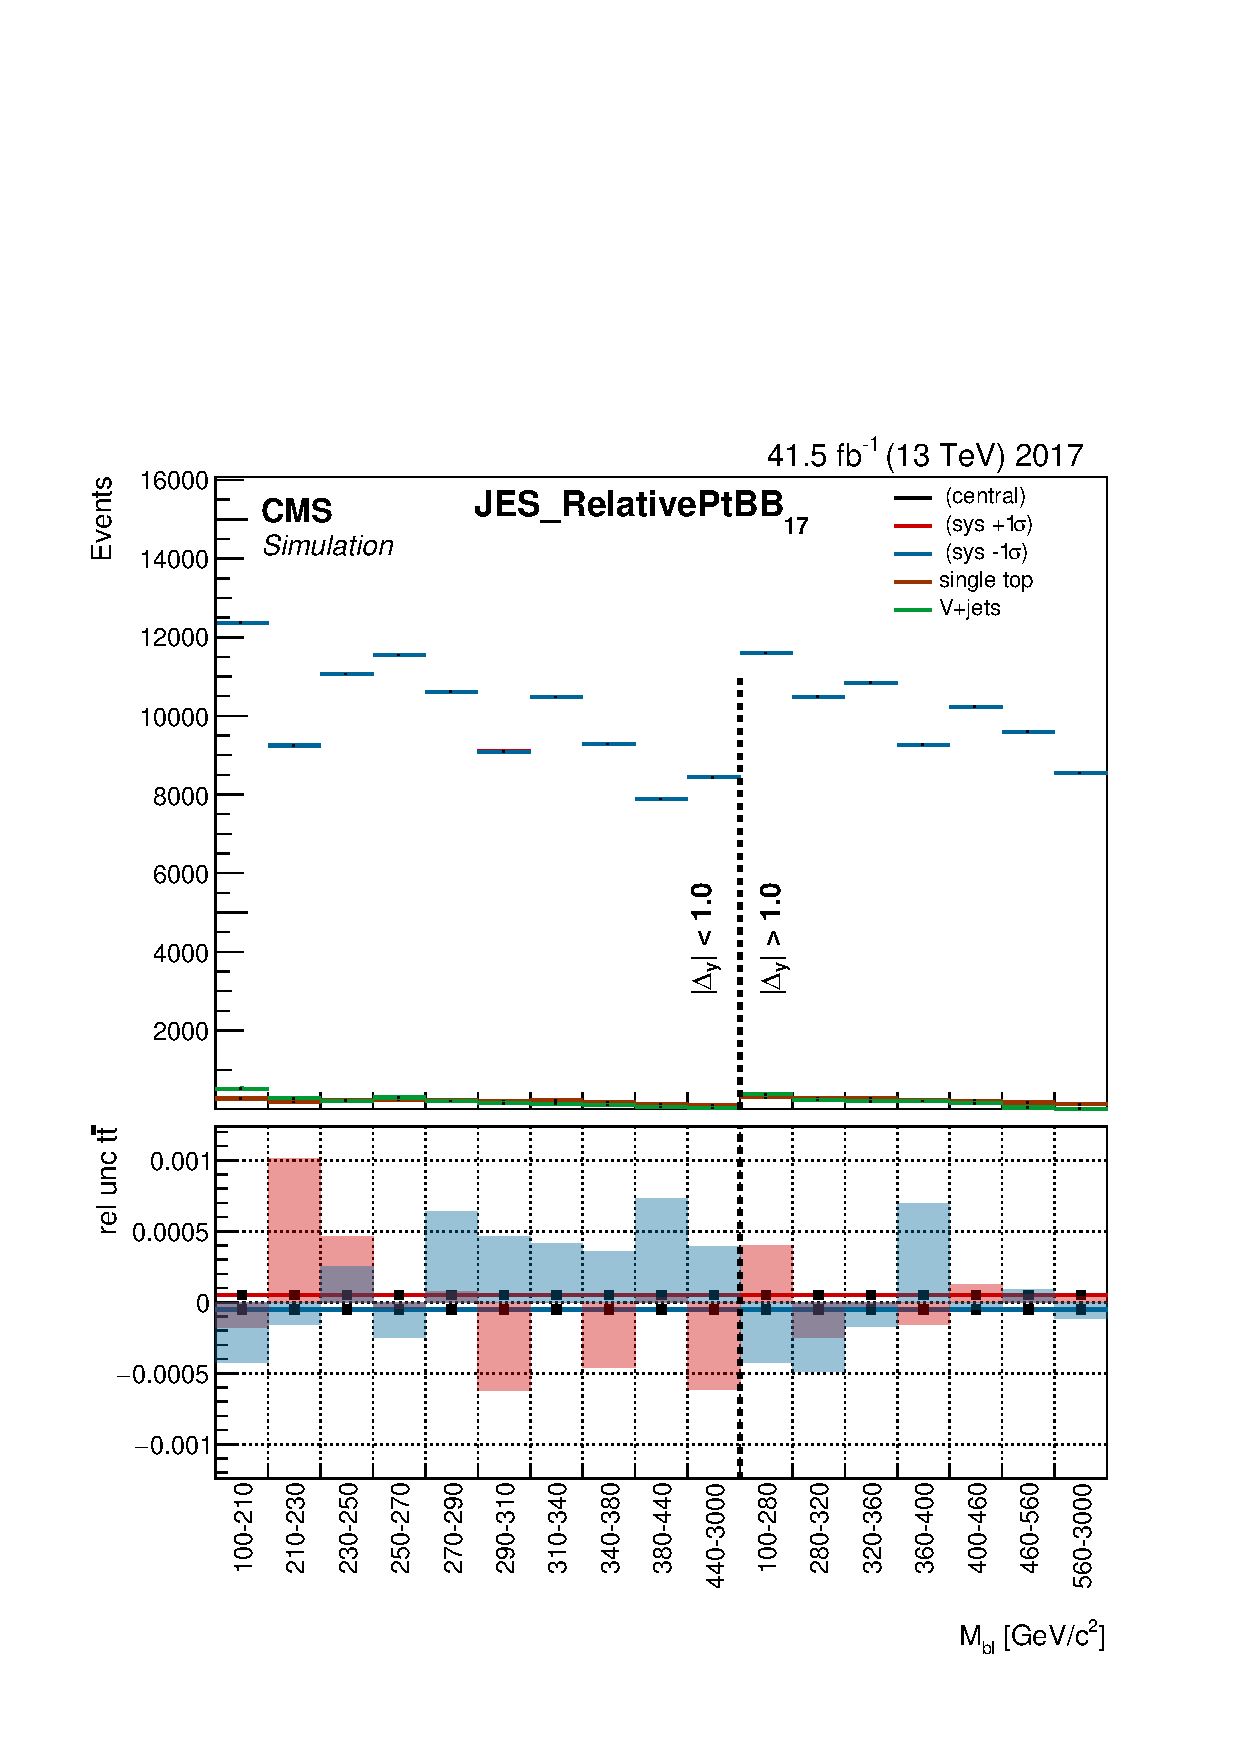
\includegraphics[width=.35\linewidth]{templates/JES_RelativePtBB_17}\hskip-.5cm
\includegraphics[width=.35\linewidth]{templates/JES_RelativePtBB_18}
\caption{JES\_RelativePtBB templates}
\label{fig:JES-RelativePtBB_template}
\end{figure}

\begin{figure} \centering
\includegraphics[width=.35\linewidth]{templates/JES_RelativePtEC1_16}\hskip-.5cm
\includegraphics[width=.35\linewidth]{templates/JES_RelativePtEC1_17}\hskip-.5cm
\includegraphics[width=.35\linewidth]{templates/JES_RelativePtEC1_18}
\caption{JES\_RelativePtEC1 templates}
\label{fig:JES-RelativePtEC1_template}
\end{figure}

\begin{figure} \centering
\includegraphics[width=.35\linewidth]{templates/JES_RelativePtEC2_16}\hskip-.5cm
\includegraphics[width=.35\linewidth]{templates/JES_RelativePtEC2_17}\hskip-.5cm
\includegraphics[width=.35\linewidth]{templates/JES_RelativePtEC2_18}
\caption{JES\_RelativePtEC2 templates}
\label{fig:JES-RelativePtEC2_template}
\end{figure}

\begin{figure} \centering
\includegraphics[width=.35\linewidth]{templates/JES_RelativePtHF_16}\hskip-.5cm
\includegraphics[width=.35\linewidth]{templates/JES_RelativePtHF_17}\hskip-.5cm
\includegraphics[width=.35\linewidth]{templates/JES_RelativePtHF_18}
\caption{JES\_RelativePtHF templates}
\label{fig:JES-RelativePtHF_template}
\end{figure}

\begin{figure} \centering
\includegraphics[width=.35\linewidth]{templates/JES_RelativeSample_16}\hskip-.5cm
\includegraphics[width=.35\linewidth]{templates/JES_RelativeSample_17}\hskip-.5cm
\includegraphics[width=.35\linewidth]{templates/JES_RelativeSample_18}
\caption{JES\_RelativeSample templates}
\label{fig:JES-RelativeSample_template}
\end{figure}

\begin{figure} \centering
\includegraphics[width=.35\linewidth]{templates/JES_SinglePionECAL_16}\hskip-.5cm
\includegraphics[width=.35\linewidth]{templates/JES_SinglePionECAL_17}\hskip-.5cm
\includegraphics[width=.35\linewidth]{templates/JES_SinglePionECAL_18}
\caption{JES\_SinglePionECAL templates}
\label{fig:JES-SinglePionECAL_template}
\end{figure}

\begin{figure} \centering
\includegraphics[width=.35\linewidth]{templates/JES_SinglePionHCAL_16}\hskip-.5cm
\includegraphics[width=.35\linewidth]{templates/JES_SinglePionHCAL_17}\hskip-.5cm
\includegraphics[width=.35\linewidth]{templates/JES_SinglePionHCAL_18}
\caption{JES\_SinglePionHCAL templates}
\label{fig:JES-SinglePionHCAL_template}
\end{figure}

\begin{figure} \centering
\includegraphics[width=.35\linewidth]{templates/JES_TimePtEta_16}\hskip-.5cm
\includegraphics[width=.35\linewidth]{templates/JES_TimePtEta_17}\hskip-.5cm
\includegraphics[width=.35\linewidth]{templates/JES_TimePtEta_18}
\caption{JES\_TimePtEta templates}
\label{fig:JES-TimePtEta_template}
\end{figure}

\begin{figure} \centering
\includegraphics[width=.35\linewidth]{templates/JER_16}\hskip-.5cm
\includegraphics[width=.35\linewidth]{templates/JER_17}\hskip-.5cm
\includegraphics[width=.35\linewidth]{templates/JER_18}
\caption{JER templates}
\label{fig:JER_template}
\end{figure}


\begin{figure} \centering
\includegraphics[width=.35\linewidth]{templates/bdec_16}\hskip-.5cm
\includegraphics[width=.35\linewidth]{templates/bdec_17}\hskip-.5cm
\includegraphics[width=.35\linewidth]{templates/bdec_18}
\caption{bdec templates}
\label{fig:bdec_template}
\end{figure}

\begin{figure} \centering
\includegraphics[width=.35\linewidth]{templates/bfrag_16}\hskip-.5cm
\includegraphics[width=.35\linewidth]{templates/bfrag_17}\hskip-.5cm
\includegraphics[width=.35\linewidth]{templates/bfrag_18}
\caption{bfrag templates}
\label{fig:bfrag_template}
\end{figure}

\begin{figure} \centering
\includegraphics[width=.35\linewidth]{templates/btag_16}\hskip-.5cm
\includegraphics[width=.35\linewidth]{templates/btag_17}\hskip-.5cm
\includegraphics[width=.35\linewidth]{templates/btag_18}
\caption{btag templates}
\label{fig:btag_template}
\end{figure}

\begin{figure} \centering
\includegraphics[width=.35\linewidth]{templates/elrec_16}\hskip-.5cm
\includegraphics[width=.35\linewidth]{templates/elrec_17}\hskip-.5cm
\includegraphics[width=.35\linewidth]{templates/elrec_18}
\caption{elrec templates}
\label{fig:elrec_template}
\end{figure}

\begin{figure} \centering
\includegraphics[width=.35\linewidth]{templates/eltrg_16}\hskip-.5cm
\includegraphics[width=.35\linewidth]{templates/eltrg_17}\hskip-.5cm
\includegraphics[width=.35\linewidth]{templates/eltrg_18}
\caption{eltrg templates}
\label{fig:eltrg_template}
\end{figure}

% \begin{figure} \centering
% \includegraphics[width=.35\linewidth]{templates/flatsys18_16}\hskip-.5cm
% \includegraphics[width=.35\linewidth]{templates/flatsys18_17}\hskip-.5cm
% \includegraphics[width=.35\linewidth]{templates/flatsys18_18}
% \caption{flatsys18 templates}
% \label{fig:flatsys18_template}
% \end{figure}

\begin{figure} \centering
\includegraphics[width=.35\linewidth]{templates/fs_16}\hskip-.5cm
\includegraphics[width=.35\linewidth]{templates/fs_17}\hskip-.5cm
\includegraphics[width=.35\linewidth]{templates/fs_18}
\caption{fs templates}
\label{fig:fs_template}
\end{figure}

\begin{figure} \centering
\includegraphics[width=.35\linewidth]{templates/fsr_16}\hskip-.5cm
\includegraphics[width=.35\linewidth]{templates/fsr_17}\hskip-.5cm
\includegraphics[width=.35\linewidth]{templates/fsr_18}
\caption{fsr templates}
\label{fig:fsr_template}
\end{figure}

\begin{figure} \centering
\includegraphics[width=.35\linewidth]{templates/hd_16}\hskip-.5cm
\includegraphics[width=.35\linewidth]{templates/hd_17}\hskip-.5cm
\includegraphics[width=.35\linewidth]{templates/hd_18}
\caption{hd templates}
\label{fig:hd_template}
\end{figure}

\begin{figure} \centering
\includegraphics[width=.35\linewidth]{templates/isr_16}\hskip-.5cm
\includegraphics[width=.35\linewidth]{templates/isr_17}\hskip-.5cm
\includegraphics[width=.35\linewidth]{templates/isr_18}
\caption{isr templates}
\label{fig:isr_template}
\end{figure}

\begin{figure} \centering
\includegraphics[width=.35\linewidth]{templates/ltag_16}\hskip-.5cm
\includegraphics[width=.35\linewidth]{templates/ltag_17}\hskip-.5cm
\includegraphics[width=.35\linewidth]{templates/ltag_18}
\caption{ltag templates}
\label{fig:ltag_template}
\end{figure}




\begin{figure} \centering
\includegraphics[width=.32\linewidth]{templates/mtop_16_old}
\includegraphics[width=.32\linewidth]{templates/mtop_17_old}
\includegraphics[width=.32\linewidth]{templates/mtop_18_old}
\caption{mtop original templates. One can see common features, but the templates are too noisy for the smoothing to yield a reasonable shape. These are NOT included in the fit}
\label{fig:mtop_template_old}
\end{figure}

\begin{figure} \centering
\includegraphics[width=.32\linewidth]{templates/mtop_16}
\includegraphics[width=.32\linewidth]{templates/mtop_17}
\includegraphics[width=.32\linewidth]{templates/mtop_18}
\caption{mtop templates after combining all 3 years to make a single template. After combining and smoothing, we see a reasonable shape effect which captures the features shared between the 3 templates in Fig. \ref{fig:mtop_template_old}. Thus, one shape is used for all 3 years.}

\label{fig:mtop_template}
\end{figure}

\begin{figure} \centering
\includegraphics[width=.35\linewidth]{templates/murec_16}\hskip-.5cm
\includegraphics[width=.35\linewidth]{templates/murec_17}\hskip-.5cm
\includegraphics[width=.35\linewidth]{templates/murec_18}
\caption{murec templates}
\label{fig:murec_template}
\end{figure}

\begin{figure} \centering
\includegraphics[width=.35\linewidth]{templates/mutrg_16}\hskip-.5cm
\includegraphics[width=.35\linewidth]{templates/mutrg_17}\hskip-.5cm
\includegraphics[width=.35\linewidth]{templates/mutrg_18}
\caption{mutrg templates}
\label{fig:mutrg_template}
\end{figure}

\begin{figure} \centering
\includegraphics[width=.35\linewidth]{templates/prefire_16}\hskip-.5cm
\includegraphics[width=.35\linewidth]{templates/prefire_17}\hskip-.5cm
\caption{prefire templates}
\label{fig:pprefire_template}
\end{figure}

\begin{figure} \centering
\includegraphics[width=.35\linewidth]{templates/pdf0_16}\hskip-.5cm
\includegraphics[width=.35\linewidth]{templates/pdf0_17}\hskip-.5cm
\includegraphics[width=.35\linewidth]{templates/pdf0_18}
\caption{pdf0 templates}
\label{fig:pdf0_template}
\end{figure}

\begin{figure} \centering
\includegraphics[width=.35\linewidth]{templates/pdf1_16}\hskip-.5cm
\includegraphics[width=.35\linewidth]{templates/pdf1_17}\hskip-.5cm
\includegraphics[width=.35\linewidth]{templates/pdf1_18}
\caption{pdf1 templates}
\label{fig:pdf1_template}
\end{figure}

\begin{figure} \centering
\includegraphics[width=.35\linewidth]{templates/pdf2_16}\hskip-.5cm
\includegraphics[width=.35\linewidth]{templates/pdf2_17}\hskip-.5cm
\includegraphics[width=.35\linewidth]{templates/pdf2_18}
\caption{pdf2 templates}
\label{fig:pdf2_template}
\end{figure}

\begin{figure} \centering
\includegraphics[width=.35\linewidth]{templates/pdf3_16}\hskip-.5cm
\includegraphics[width=.35\linewidth]{templates/pdf3_17}\hskip-.5cm
\includegraphics[width=.35\linewidth]{templates/pdf3_18}
\caption{pdf3 templates}
\label{fig:pdf3_template}
\end{figure}

\begin{figure} \centering
\includegraphics[width=.35\linewidth]{templates/pdf4_16}\hskip-.5cm
\includegraphics[width=.35\linewidth]{templates/pdf4_17}\hskip-.5cm
\includegraphics[width=.35\linewidth]{templates/pdf4_18}
\caption{pdf4 templates}
\label{fig:pdf4_template}
\end{figure}

\begin{figure} \centering
\includegraphics[width=.35\linewidth]{templates/pdf5_16}\hskip-.5cm
\includegraphics[width=.35\linewidth]{templates/pdf5_17}\hskip-.5cm
\includegraphics[width=.35\linewidth]{templates/pdf5_18}
\caption{pdf5 templates}
\label{fig:pdf5_template}
\end{figure}

\begin{figure} \centering
\includegraphics[width=.35\linewidth]{templates/pdf6_16}\hskip-.5cm
\includegraphics[width=.35\linewidth]{templates/pdf6_17}\hskip-.5cm
\includegraphics[width=.35\linewidth]{templates/pdf6_18}
\caption{pdf6 templates}
\label{fig:pdf6_template}
\end{figure}

\begin{figure} \centering
\includegraphics[width=.35\linewidth]{templates/pdf7_16}\hskip-.5cm
\includegraphics[width=.35\linewidth]{templates/pdf7_17}\hskip-.5cm
\includegraphics[width=.35\linewidth]{templates/pdf7_18}
\caption{pdf7 templates}
\label{fig:pdf7_template}
\end{figure}

\begin{figure} \centering
\includegraphics[width=.35\linewidth]{templates/pdf8_16}\hskip-.5cm
\includegraphics[width=.35\linewidth]{templates/pdf8_17}\hskip-.5cm
\includegraphics[width=.35\linewidth]{templates/pdf8_18}
\caption{pdf8 templates}
\label{fig:pdf8_template}
\end{figure}

\begin{figure} \centering
\includegraphics[width=.35\linewidth]{templates/pdf9_16}\hskip-.5cm
\includegraphics[width=.35\linewidth]{templates/pdf9_17}\hskip-.5cm
\includegraphics[width=.35\linewidth]{templates/pdf9_18}
\caption{pdf9 templates}
\label{fig:pdf9_template}
\end{figure}


\begin{figure} \centering
\includegraphics[width=.35\linewidth]{templates/pdf_as_16}\hskip-.5cm
\includegraphics[width=.35\linewidth]{templates/pdf_as_17}\hskip-.5cm
\includegraphics[width=.35\linewidth]{templates/pdf_as_18}
\caption{pdf-as template }
\label{fig:pdfas_template}
\end{figure}


\clearpage



\begin{figure} \centering
\includegraphics[width=.35\linewidth]{templates/pu_16}\hskip-.5cm
\includegraphics[width=.35\linewidth]{templates/pu_17}\hskip-.5cm
\includegraphics[width=.35\linewidth]{templates/pu_18}
\caption{pu templates}
\label{fig:pu_template}
\end{figure}

\begin{figure} \centering
\includegraphics[width=.35\linewidth]{templates/rs_16}\hskip-.5cm
\includegraphics[width=.35\linewidth]{templates/rs_17}\hskip-.5cm
\includegraphics[width=.35\linewidth]{templates/rs_18}
\caption{rs templates}
\label{fig:rs_template}
\end{figure}

\begin{figure} \centering
\includegraphics[width=.35\linewidth]{templates/rsfs_16}\hskip-.5cm
\includegraphics[width=.35\linewidth]{templates/rsfs_17}\hskip-.5cm
\includegraphics[width=.35\linewidth]{templates/rsfs_18}
\caption{rsfs templates}
\label{fig:rsfs_template}
\end{figure}





\begin{figure} \centering
\includegraphics[width=.35\linewidth]{templates/tune_16}\hskip-.5cm
\includegraphics[width=.35\linewidth]{templates/tune_17}\hskip-.5cm
\includegraphics[width=.35\linewidth]{templates/tune_18}
\caption{tune templates}
\label{fig:tune_template}
\end{figure}



\clearpage

\bibliographystyle{auto_generated}
\bibliography{sources.bib}

\end{document}